% Tipo di documento. L'uso di twoside implica che i capitoli inizino sempre con la prima pagina a sinistra, eventualmente lasciando una pagina vuota nel capitolo precedente. Se questa cosa è fastidiosa, è possibile rimuoverlo. 
\documentclass[a4paper,openright]{report}

% Dimensione dei margini
\usepackage[a4paper,top=3cm,bottom=3cm,left=3cm,right=3cm]{geometry} 
% Dimensione del font
\usepackage[fontsize=13pt]{scrextend}
% Lingua del testo
\usepackage[english]{babel}
% Lingua per la bibliografia
\usepackage[fixlanguage]{babelbib}
% Codifica del testo
\usepackage[utf8]{inputenc} 
% Encoding del testo
\usepackage[T1]{fontenc}
% Permette di generare testo fittizio. Mi è stato utile 
% per capire quale sarebbe stata l'impostazione del 
% testo nella pagina prima che scrivessi un determinato paragrafo
\usepackage{lipsum}
% Per ruotare le immagini
\usepackage{rotating}
% Per modificare l'header delle pagine 
\usepackage{fancyhdr}      

% wrap images package
\usepackage{wrapfig}
% \makeFNbelow by default 
\usepackage{ftnxtra}
\usepackage{fnpos}
%caption package
\usepackage{caption}
% Librerie matematiche
\usepackage{amssymb}
\usepackage{amsmath}
\usepackage{amsthm}         

% Uso delle immagini
\usepackage{graphicx}
% Uso dei colori
\usepackage[dvipsnames]{xcolor}         
% Uso dei listing per il codice
\usepackage{listings}          
% Per inserire gli hyperlinks tra i vari elementi del testo 
\PassOptionsToPackage{hyphens}{url}
\usepackage{hyperref}     
% Diversi tipi di sottolineature
\usepackage[normalem]{ulem}
% Custom colors
\usepackage{color}
%Immagini all'interno di liste
\usepackage{float,graphicx}
%Contiene simboli
\usepackage{fontawesome}
%contiene faccine
\usepackage{wasysym}

\usepackage[verbose]{newunicodechar}

% -----------------------------------------------------------------

% Modifica lo stile dell'header
\pagestyle{fancy}
\fancyhf{}
\lhead{\rightmark}
\rhead{\textbf{\thepage}}
\fancyfoot{}
\setlength{\headheight}{12.5pt}

% Rimuove il numero di pagina all'inizio dei capitoli
\fancypagestyle{plain}{
  \fancyfoot{}
  \fancyhead{}
  \renewcommand{\headrulewidth}{0pt}
}

% Default fixed font does not support bold face
\DeclareFixedFont{\ttb}{T1}{txtt}{bx}{n}{12} % for bold
\DeclareFixedFont{\ttm}{T1}{txtt}{m}{n}{12}  % for normal

%definizione di terminale su Latex
\definecolor{mygreen}{rgb}{0,0.6,0}
\definecolor{mygray}{rgb}{0.5,0.5,0.5}
\definecolor{mymauve}{rgb}{0.58,0,0.82}
\definecolor{terminalbgcolor}{HTML}{330033}
\definecolor{terminalrulecolor}{HTML}{000099}

\newcommand{\lstconsolestyle}{
    \lstset{ %lstset legato a output
    	backgroundcolor=\color{terminalbgcolor},
    	basicstyle=\color{white}\fontfamily{fvm}\footnotesize\selectfont\scriptsize,
    	breakatwhitespace=false,  
    	breaklines=true,
    	captionpos=b,
    	commentstyle=\color{mygreen},
    	deletekeywords={...},
    	escapeinside={\%*}{*)},
    	extendedchars=true,
    	frame=single,
    	keepspaces=true,
    	keywordstyle=\color{blue},
    	language=none,
    	morekeywords={*,...},
    	numbers=none,
    	numbersep=5pt,
        framerule=2pt,
    	numberstyle=\color{mygray}\tiny\selectfont,
    	rulecolor=\color{terminalrulecolor},
    	showspaces=false,
    	showstringspaces=false,
    	showtabs=false,
    	stepnumber=2,
    	stringstyle=\color{green},
    	tabsize=2,
        inputencoding=utf8,
        extendedchars=true,
        literate={·}{$\cdot$}1 {✅}{\faCheckSquare}1 {✔}{\faCheck}1
    }
}

\newcommand\lstJavaScriptcodestyle{
    \lstset{
      backgroundcolor=\color{white},
      breakatwhitespace=true,  
      breaklines=true,
      frame=tb,
        framerule=0.5pt,
        rulecolor = \color{black},
      numbers=left,
      language=JavaScript,
      aboveskip=3mm,
      belowskip=3mm, 
      showstringspaces=false,
      columns=flexible,
      basicstyle={\small\ttfamily},
      numbers=left,
      stepnumber=1,
      numberstyle=\tiny\color{gray},
      keywordstyle=\color{blue},
      commentstyle=\color{dkgreen},
      stringstyle=\color{mauve},
      rulecolor=\color{black},
      breaklines=true,
      breakatwhitespace=true,
      tabsize=3
    }
}

\definecolor{deepblue}{rgb}{0,0,0.5}
\definecolor{deepred}{rgb}{0.6,0,0}
\definecolor{deepgreen}{rgb}{0,0.5,0}

\newcommand\lstPythoncodestyle{
    \lstset{ %lstset legato a output
    	language=Python,
        backgroundcolor=\color{white},
        basicstyle=\ttm,
        morekeywords={self},              % Add keywords here
        keywordstyle=\ttb\color{deepblue},
        emph={load_dotenv, main, buyerTestCase, generatePlots},          % Custom highlighting
        emphstyle=\ttb\color{deepred},    % Custom highlighting style
        stringstyle=\color{deepgreen},
        frame=tb,                         % Any extra options here
        framerule=1pt,
        rulecolor = \color{black},
        showstringspaces=false
    }
}

%lstset legato a codice
\definecolor{dkgreen}{rgb}{0,0.6,0}
\definecolor{gray}{rgb}{0.5,0.5,0.5}
\definecolor{mauve}{rgb}{0.58,0,0.82}

\lstset{frame=tb,
  %language=Java,
  inputencoding=utf8,
  aboveskip=3mm,
  belowskip=3mm,
  showstringspaces=false,
  columns=flexible,
  basicstyle={\scriptsize\ttfamily},
  numbers=none,
  numberstyle=\tiny\color{gray},
  keywordstyle=\color{blue},
  commentstyle=\color{dkgreen},
  stringstyle=\color{mauve},
  breaklines=true,
  breakatwhitespace=true,
  tabsize=3
}

%definisco linguaggio JavaScript
\lstdefinelanguage{JavaScript}{
    keywords={typeof, new, true, false, catch, function, return, null, catch, switch, var, if, in, while, do, else, case, break},
    keywordstyle=\color{blue}\bfseries,
    ndkeywords={class, export, boolean, throw, implements, import, this},
    ndkeywordstyle=\color{darkgray}\bfseries,
    identifierstyle=\color{black},
    sensitive=false,
    numbers=left,
    stepnumber=1,
    comment=[l]{//},
    morecomment=[s]{/*}{*/},
    commentstyle=\color{purple}\ttfamily,
    stringstyle=\color{red}\ttfamily,
    morestring=[b]',
    morestring=[b]"
}

%definisco linguaggio vuoto
\lstdefinelanguage{none}{
  identifierstyle=
}

% Margini prima e dopo blocchi di codice, per avere più distanza
\lstset{aboveskip=20pt,belowskip=20pt}

% Modifica dello stile dei riferimenti, con il testo in cyano
\hypersetup{
    colorlinks,
    linkcolor=black,
    citecolor=blue,
    urlcolor=cyan,
    pdftitle={Advanced Software Engineering notes},
}

% Aggiunti definizioni, teoremi, linea e listing
\newtheorem{definition}{Definizione}[section]
\newtheorem{theorem}{Teorema}[section]
\providecommand*\definitionautorefname{Definizione}
\providecommand*\theoremautorefname{Teorema}
\providecommand*{\listingautorefname}{Listing}
\providecommand*\lstnumberautorefname{Linea}

\raggedbottom

%\newcommand{\cgs}[1]{{\textcolor{brown}[\textcolor{red}{\bf{GS: }}{ \textcolor{brown}{#1]}}}}             
%\newcommand{\cmc}[1]{{\textcolor{blue}[\textcolor{magenta}{\bf{MC: }}{ \textcolor{blue}{#1]}}}}


\title{Advanced Software Engineering}
\date{September - December 2023}

\begin{document}

\author{Emiliano Sescu \\ \url{https://github.com/Faxatos}}
\maketitle
\renewcommand{\abstractname}{Abstract}
\begin{abstract}

\noindent These notes follow the structure of the course and the lessons presented by Professor Brogi. Along with the slides used in the lectures, these notes will help you prepare for the theoretical part of the exam. The topics included are:

\begin{itemize}
    \item Software Products
    \item Agile Software Engineering
    \item Features, Scenarios, and Stories
    \item Software Architecture
    \item Cloud-based Software
    \item Microservices Architecture
    \item Security and Privacy
    \item Business Process Modeling
    \item Testing
    \item DevOps and Code Management
    \item Edge-Cloud Continuum
    \item Quantum Software Engineering
\end{itemize}

\noindent These notes are available for free! If you find them helpful, please consider leaving a follow on my GitHub account: \url{https://github.com/Faxatos} \smiley{}

\end{abstract}

\newpage

\tableofcontents

% Rimuovere se non si vuole la tabella delle figure
%\listoffigures

%\chapter{Introduzione}



\chapter{Software products}

\section{Project-based Software Engineering}
\textbf{Project-based software engineering} was the first form of software engineering. It starts from the desire of the customers, and at the end of the project you obtain software to be given to the user.

Developers usually try to transition from products originated from different customer to a single product that satisfy all types of customers. The problem with project-based software engineering was that the customer have to generate the requirements in a certain format about things that they generally don't understand. The customer doesn't think in terms of software requirements (requirements specify what is the software we need to implement), so it forces the customer to generate them. The requirements, also, are not static: they change each time we meet customers, because they understand what the software can do for them.

\begin{figure} [H]
    \centering
    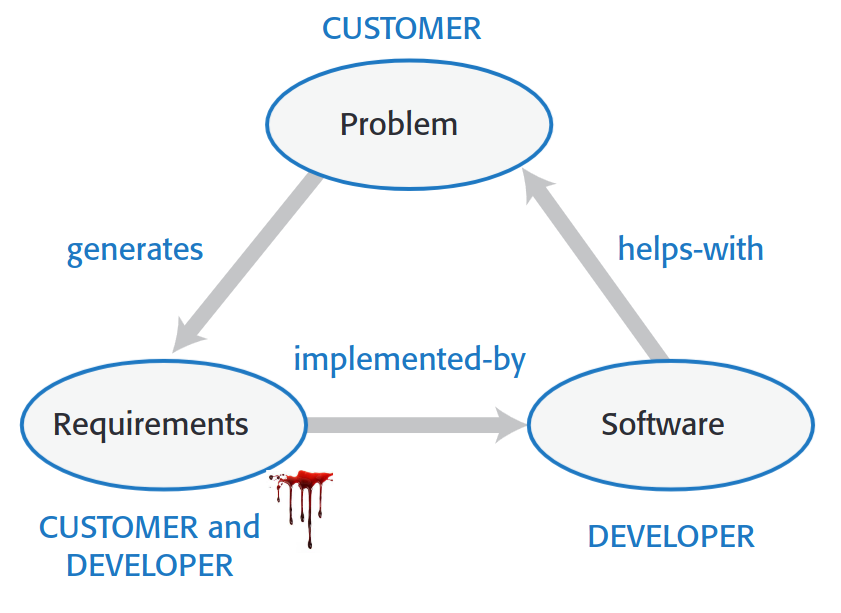
\includegraphics[width=0.6\textwidth]{images/Products/ProductsSE.png}
    \caption{Life cycle of project-based software engineering}
    \label{fig:ProductsSE}
\end{figure} 

\noindent 
For most business, users don't need customized software, but they need generalized software.

\section{Product-based Software Engineering}

In \textbf{product-based software engineering} the group of developers decides which are the software features, and how the software will change. The customer disappears from the cicle, so the developer choose which project they will build. The developers must identify features that meet the needs of the customers.

\begin{figure} [H]
    \centering
    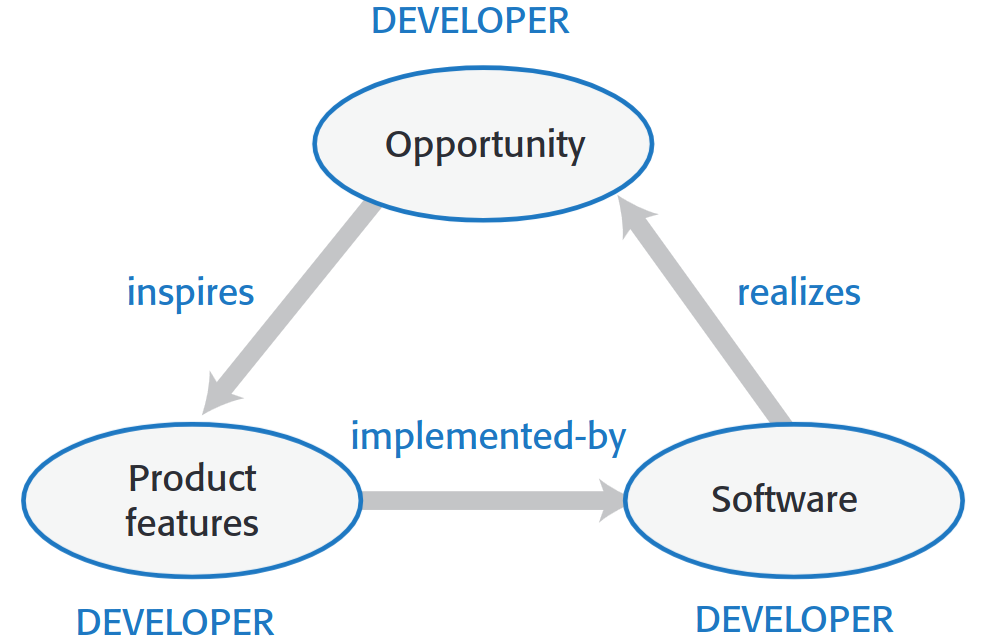
\includegraphics[width=0.6\textwidth]{images/Products/productbasedSE.png}
    \caption{Life cycle of product-based software engineering}
    \label{fig:productbasedSE}
\end{figure} 

One of the products based software engineering requirements is that we need to develop software quickly in order to not let someone else steal that market share. That's why time is critical, and that's why agile methods are used. \\

There are 3 types of \textbf{software execution models}: 
\begin{itemize}
    \item \textbf{Stand-alone execution}: The user interface, functionalities, and data are all stored on the user's computer. The vendor is responsible for creating and sending updates.
    \item \textbf{Hybrid execution}: Part of the application is on the end-user device (user interface, user data, and all updates from the vendor), and part is on the vendor's server (business logic and user data backups).
    \item \textbf{Software as a service} (SaaS): The user doesn't need to install anything (they just have an interface), meaning the program is hosted on the vendor's server. This makes it easier to manage and update the program without needing to distribute it. 
\end{itemize}

\begin{figure} [H]
    \centering
    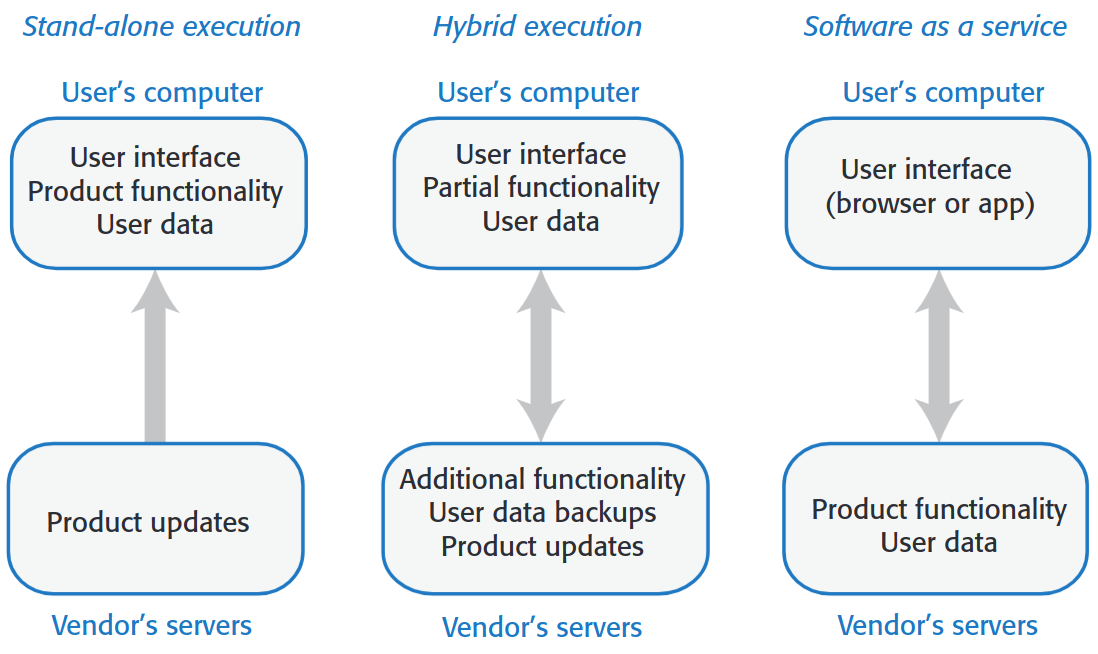
\includegraphics[width=0.66\textwidth]{images/Products/executionmodels.png}
    \label{fig:executionmodels}
    \caption{Execution models}
\end{figure} 

\section{Product vision}

For any new promising software program, there should be a \textbf{vision for the program}: \textcolor{green}{Who} are the targeted customers? \textcolor{brown}{What} is the product to be developed? \textcolor{red}{Why} should customers buy the product?

\noindent For programmers, it's easier to build cards with the following structure:
\newline \noindent \textcolor{green}{FOR (target customer)} \textcolor{green}{WHO (statement of the need or opportunity)}
\newline \noindent \textcolor{brown}{THE (product name) is a (product category)} \textcolor{brown}{THAT (key benefit, compelling reason to buy)}
\newline \noindent \textcolor{red}{UNLIKE (primary competitive alternative)} \textcolor{red}{OUR PRODUCT (statement of primary differentiation)}\\

These are the relevant aspects to building a product vision:
\begin{itemize}
    \item \textbf{Domain experience}: The product developers may work in a particular area (such as marketing and sales) and understand the software support they need. They may be frustrated by the deficiencies in the software they use and see opportunities for an improved system.
    \item \textbf{Product experience}: Users of existing software (such as word processing software) may identify simpler and better ways to provide comparable functionality and propose a new system to implement this. New products can also take advantage of recent technological developments (such as speech interfaces).
    \item \textbf{Customer experience}: Software developers may have extensive discussions with prospective customers to understand the problems they face, as well as constraints, such as interoperability, that limit their flexibility to buy new software. Developers also consider the critical attributes customers need in the software.
    \item \textbf{Prototyping and experimentation}: Developers may have an idea for software but need to develop a better understanding of the concept and what is involved in turning it into a product. Prototyping allows for the exploration of new ideas and feedback from customers (since customers think in terms of functionalities), guiding the path for the next prototype.
\end{itemize}

\section{Software product management}

The \textbf{Product Manager} must ensure that the development team implements features that deliver real value to customers. They must also find a balance between these three forces (we'll see how some Agile techniques help the Product Manager achieve these results):

\begin{itemize}
    \item \textbf{Business needs}: The entire product development process must be managed while considering business needs. The PM needs to ensure that the product satisfies the goals of both the customer and the company.
    \item \textbf{Customer experience}: Regularly gather feedback from customers to understand their experience with the product.
    \item \textbf{Technology constraints}: Consider the various technology constraints the company may have. The Product Manager must take into account the type of hardware and technology the customer already uses.
\end{itemize}

\begin{figure} [H]
    \centering
    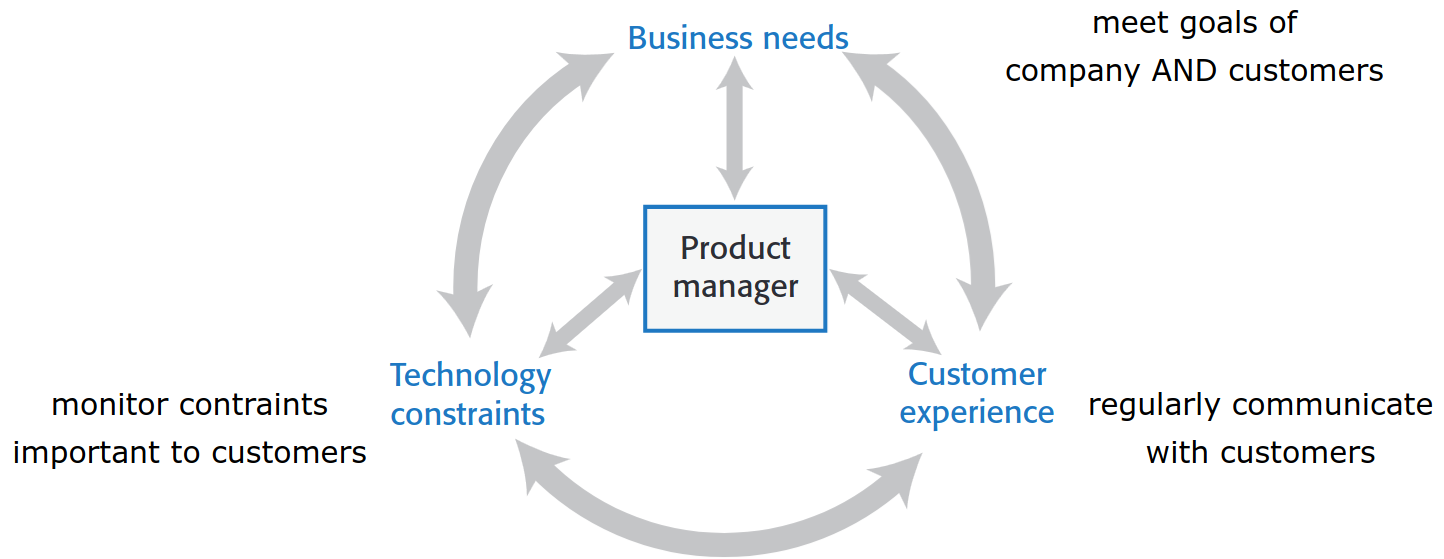
\includegraphics[width=0.73\textwidth]{images/Products/productmanager.png}
    \caption{Product Manager duties}
    \label{fig:productmanager}
\end{figure}

The Product Manager will have some \textbf{technical interactions} such as:
\begin{itemize}
    \item The \textbf{Product roadmap}, which includes setting goals, milestones, success criteria, and alternative paths in case the goals are not reached.
    \item \textbf{User stories and scenarios} to identify product features.
    \item The \textbf{Product backlog}, a to-do list for completing project development.
    \item \textbf{Acceptance testing}, which is used throughout the product lifecycle to verify that releases meet the set goals.
    \item \textbf{Customer testing}, which involves gathering feedback on usability and features.
    \item \textbf{UI design} to ensure simplicity and a natural user interface.
\end{itemize}

%he especially need to make sure that the product meets the goal of the customers. 1:00:00 for full image expl.

\chapter{Agile Software Engineering}
For the past 50 years, software engineering was primarily focused on plan-driven development, which included:

\begin{itemize}
    \item Detailed project planning (a particularly heavy part)
    \item Requirement specification (also a very intensive part)
    \item Analysis and design methods
    \item Comprehensive system documentation
    \item Formal quality assurance
\end{itemize}

\noindent At the beginning of the new millennium, a manifesto for agile software development was published, emphasizing:

\begin{itemize}
    \item \textbf{Individuals and interactions} over processes and tools
    \item \textbf{Working software} over comprehensive documentation (even though documentation is useful for those who will modify the code later, making it detailed is very costly)
    \item \textbf{Customer collaboration} over contract negotiation (to include the customer in the software development process)
    \item \textbf{Responding to change} over following a plan (since no one can predict the future)
\end{itemize}

The radically new perspective of Agile is to move away from thinking about applications the way they were previously thought of and instead try to align with how users think about the system (as a set of functionalities). One of the Agile principles is \textbf{Incremental Development}: it involves selecting a few functionalities and then implementing them.

\begin{figure} [H]
    \centering
    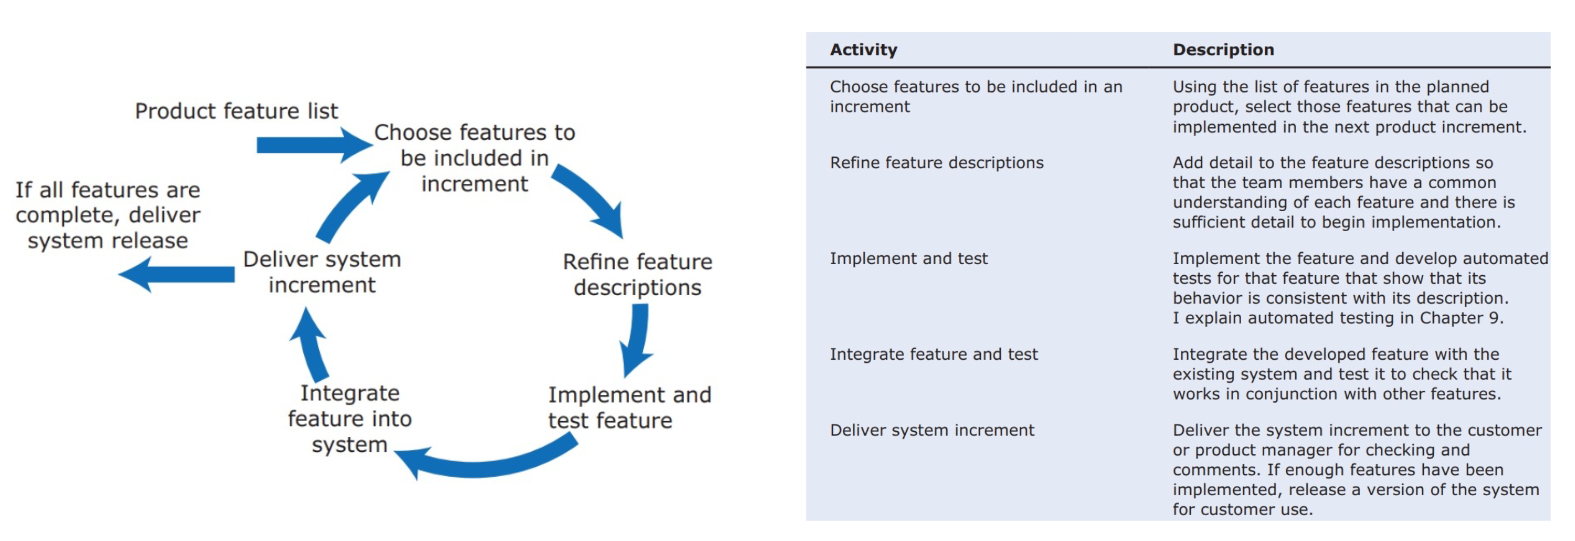
\includegraphics[width=1\textwidth]{images/Agile/CICD.png}
    \caption{Continuous Integration and Continuous Deployment cycle}
    \label{fig:CICD}
\end{figure}

This cycle is then repeated until the final system is completed. These rounds, where we implement features, can sometimes fail, either due to a misinterpretation of required functionalities or because the customer changes their mind. This process, which can be visualized as a pipeline, is called \textbf{Continuous Integration and Continuous Delivery/Continuous Deployment} (CICD). \\

\noindent Here are twelve more \textbf{Agile principles}:

\begin{itemize}
    \item Our highest priority is to satisfy the customer through \textit{early and continuous delivery of valuable software}. (as soon as there's a usable piece of software, it should be deployed)
    \item \textbf{Welcome changing requirements}, even late in development. Agile processes harness change for the customer's competitive advantage. (it is unrealistic to have a full and complete set of functionalities from users at the beginning of development. Programmers should adopt a mindset that embraces changing requirements)
    \item \textbf{Deliver working software frequently}, from a couple of weeks to a couple of months, with a preference for the shorter timescale. (CICD pipeline)
    \item Business people and developers must \textbf{work together} daily throughout the project.
    \item The most efficient and effective method of conveying information to and within a development team is face-to-face conversation.
    \item \textbf{Working software is the primary measure of progress}. (not the delivery of new documentation or specifications)
    \item Agile processes promote sustainable development. The sponsors, developers, and users should be able to maintain a constant pace indefinitely.
    \item Continuous attention to technical excellence and good design enhances agility.
    \item \textbf{Simplicity}—the art of maximizing the amount of work not done—is essential.
    \item The best architectures, requirements, and designs emerge from \textbf{self-organizing teams}. (rather than having separate teams in different rooms)
    \item At regular intervals, the \textbf{team reflects} on how to become more effective, then tunes and adjusts its behavior accordingly. (periodically evaluate and adjust practices)
\end{itemize}


\section{Extreme Programming}

Extreme Programming (XP) is one of the techniques proposed as part of Agile methodology. The key points of XP are shown in the following image:

\begin{figure} [H]
    \centering
    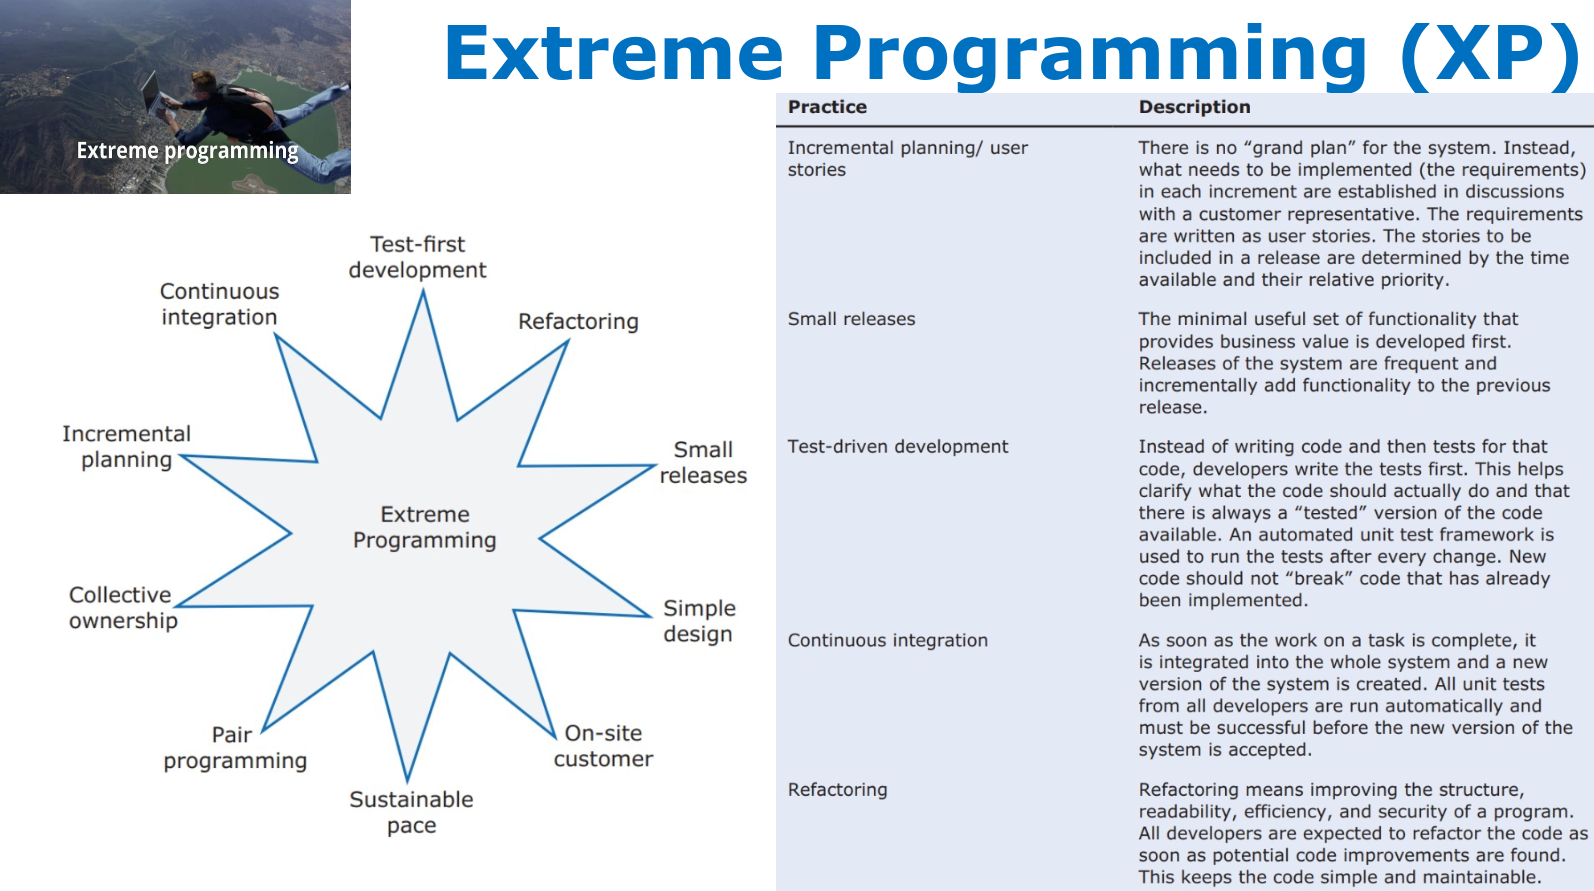
\includegraphics[width=1\textwidth]{images/Agile/ExtremeProgramming.png}
    \caption{Extreme Programming principles}
    \label{fig:extremeprogramming}
\end{figure} 

\section{Scrum}

Scrum is a \textbf{lightweight framework} that helps individuals, teams, and organizations generate value through adaptive solutions to complex problems. The Scrum framework contains a set of principles and rules to follow in order to achieve a common goal.

The motivation behind Scrum is that software company managers need information that helps them understand the cost of developing a software product, the development timeline, and when the product can be brought to market. Plan-driven development provides this information through long-term development plans that identify deliverables—items the team will deliver and when these will be delivered. However, plans always change, making long-term plans unreliable, except for short-term planning.

Scrum is based on \textbf{Empiricism}, which asserts that knowledge comes from experience and that decisions should be made based on observation. It is also rooted in \textbf{Lean thinking}, which focuses on reducing waste and emphasizing essentials. Scrum employs an iterative, incremental approach to optimize predictability and control risk. The pillars of Scrum are:

\begin{itemize}
    \item \textbf{Transparency}: The progress and work should be visible to those performing the work and those receiving the work.
    \item \textbf{Inspection}: Scrum artifacts and progress toward agreed goals must be frequently and diligently inspected to detect potentially undesirable variances or problems.
    \item \textbf{Adaptation}: If any aspects of a process deviate (e.g., new requirements) beyond acceptable limits, or if the resulting product is unacceptable, the process being applied or the materials being produced must be adjusted. These adjustments should be made as soon as possible to minimize further deviation.
\end{itemize}

Successful use of Scrum depends on people becoming more proficient in living its five core values: \textbf{Commitment} (respect deadlines), \textbf{Focus}, \textbf{Openness} (being open to new solutions), \textbf{Respect} (for teammates and others), and \textbf{Courage} (to propose new solutions that better align the product with its vision).

\subsection{Scrum Team}

A \textbf{self-organizing team} coordinates its work by discussing tasks and reaching a consensus on who should do what. This minimizes the involvement of engineers in external interactions with management and customers. The team makes its own decisions on schedules and deliverables.

\textbf{External interactions} refer to interactions team members have with individuals outside the team. In Scrum, the idea is that developers should focus on development, while only the Scrum Master and Product Owner should handle external interactions. The goal is for the team to focus on software development without external interference or distractions.

\subsubsection{Product Owner}

The Product Owner is responsible for ensuring that the development team stays focused on building the product rather than getting sidetracked by technically interesting but less relevant work. In product development, the Product Manager typically assumes the Product Owner role. \\

Product-focused external interactions are managed by the Product Owner.

\subsubsection{Scrum Master}

The Scrum Master is an expert in Scrum whose job is to guide the team in effectively using the Scrum method. Scrum developers emphasize that the Scrum Master is not a traditional project manager but rather a coach for the team. They have authority within the team regarding how Scrum is used. In many companies, the Scrum Master also takes on some project management responsibilities. \\

In all but the smallest product development companies, development teams must report progress to company management. A self-organizing team needs to appoint someone to handle these responsibilities. Because maintaining continuity in communication with people outside the group is crucial, rotating these activities among team members is not a viable approach. Although the Scrum developers did not envision the Scrum Master also assuming project management responsibilities, in many companies, \textit{the Scrum Master takes on project management tasks} because they have the best understanding of the work in progress and are in the best position to provide accurate information and project plans. \\

Team-focused external interactions are managed by the Scrum Master.

\subsubsection{Developers}

Self-organizing teams make their own decisions, working by discussing issues and reaching a consensus. The ideal \textbf{Scrum team size} is between 5 and 8 people. Teams need to tackle diverse tasks, often requiring members with different skills, such as networking, user experience, database design, and more. They also typically include individuals with varying levels of experience. A team of 5 to 8 people is large enough to be diverse yet small enough to communicate informally and effectively, allowing for agreement on team priorities.

The advantage of a self-organizing team is that it can become cohesive and adapt to change. Because the team, rather than individuals, takes responsibility for the work, it can manage transitions when team members leave or join. Effective communication within the team means that members inevitably learn about each other’s areas of expertise. \\

The developers of Scrum assumed that teams would be co-located, working in the same space to communicate informally. Daily scrums help team members stay updated on what’s been done and what others are working on. However, two assumptions behind the daily scrum are not always correct: 
\begin{itemize}
    \item Scrum assumes that the team is made up of full-time workers sharing a workspace. In reality, team members may work part-time or in different locations. For student project teams, members may take different classes at different times.
    \item Scrum assumes that all team members can attend a morning meeting to coordinate the day’s work. However, some members may work flexible hours (e.g., due to childcare responsibilities) or may work on several projects simultaneously.
\end{itemize}

\subsection{Artifacts}

\subsubsection{Product Backlog}

The product backlog is a list of tasks that need to be completed to develop the product. This to-do list of items is reviewed and updated before each sprint.

\begin{figure} [H]
    \centering
    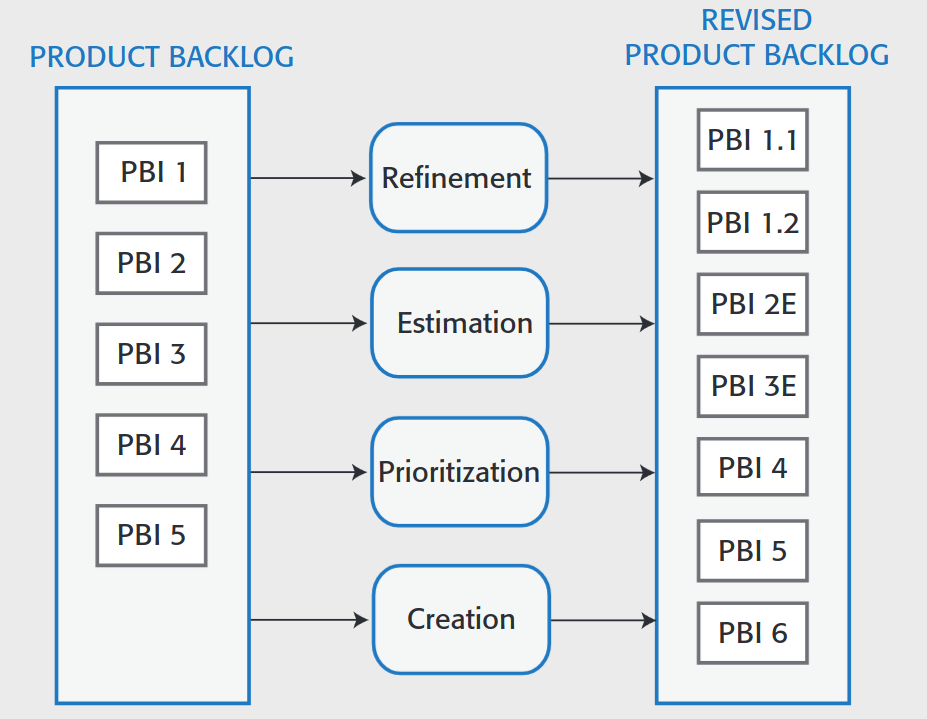
\includegraphics[width=0.8\textwidth]{images/Agile/ProductBacklog.png}
    \caption{Product backlog during the action process}
    \label{fig:productbacklog}
\end{figure} 

As illustrated in the image above, items that are to be implemented are first selected and prioritized. According to their priorities, they are sorted and will be implemented in the next sprint. Below are some examples of product backlog items:

\begin{itemize}
    \item \textit{As a teacher, I want to be able to configure the group of tools that are available to individual classes.} (feature)
    \item \textit{As a parent, I want to be able to view my children's work and the assessments made by their teachers.} (feature)
    \item \textit{As a teacher of young children, I want a pictorial interface for children with limited reading ability.} (user request)
    \item \textit{Implement encryption for all personal user data.} (engineering improvement)
\end{itemize}

\newpage

\noindent Product backlog items can exist in different states:

\begin{itemize}
	\item \textbf{Ready for consideration}: High-level ideas and feature descriptions are under consideration for inclusion in the product. These are tentative and may change or not be included in the final product.
	\item \textbf{Ready for refinement}: The team agrees that this is an important item to be implemented in the current development cycle. There is a reasonably clear definition of what is required, though further refinement is needed.
	\item \textbf{Ready for implementation}: The product backlog item has enough detail for the team to estimate the effort required and begin implementation. Dependencies on other items are also identified.
\end{itemize}

\subsubsection{Sprint Backlog}

The sprint backlog is a focused list of tasks selected from the product backlog that the team commits to completing during the sprint. It is created during sprint planning, where items are chosen based on the sprint goal and broken down into smaller, actionable tasks.

Unlike the product backlog, which contains all potential features and improvements, the sprint backlog is \textbf{limited to what can be achieved within the sprint’s time frame}. As the sprint progresses, the team updates the sprint backlog to track completed tasks and any changes that arise.

The sprint backlog helps the team stay aligned with their sprint goal and manage progress efficiently. Tools like burn-down charts are often used to visualize the remaining work and time in the sprint.

\subsection{Scrum Events}

In Scrum, software is developed in fixed-length periods called \textbf{sprints}, typically lasting 2-4 weeks. During a sprint, the team holds daily meetings (Scrums) to review progress and update the list of incomplete work items. A sprint aims to produce a ‘\textit{shippable product increment},’ meaning that the developed software should be complete and ready to deploy. Sprints are \textbf{timeboxed}, meaning development stops at the end of the sprint, regardless of whether all work has been completed. The team works on items from the product backlog during a sprint. \\

There are three main types of \textbf{sprint activities}:
\begin{itemize}
    \item \textbf{Sprint Planning}: The team selects the work items to be completed during the sprint, and if necessary, refines them to create a sprint backlog. This planning session should not last longer than a day at the start of the sprint.
    \item \textbf{Sprint Execution}: The team works to implement the sprint backlog items. If it becomes impossible to complete all items, the sprint is not extended; instead, unfinished items are returned to the product backlog for future sprints.
    \item \textbf{Sprint Review}: The team and possibly external stakeholders review the completed work. They reflect on what went well, what went wrong, and how to improve their work processes.
\end{itemize}

\begin{figure} [H]
    \centering
    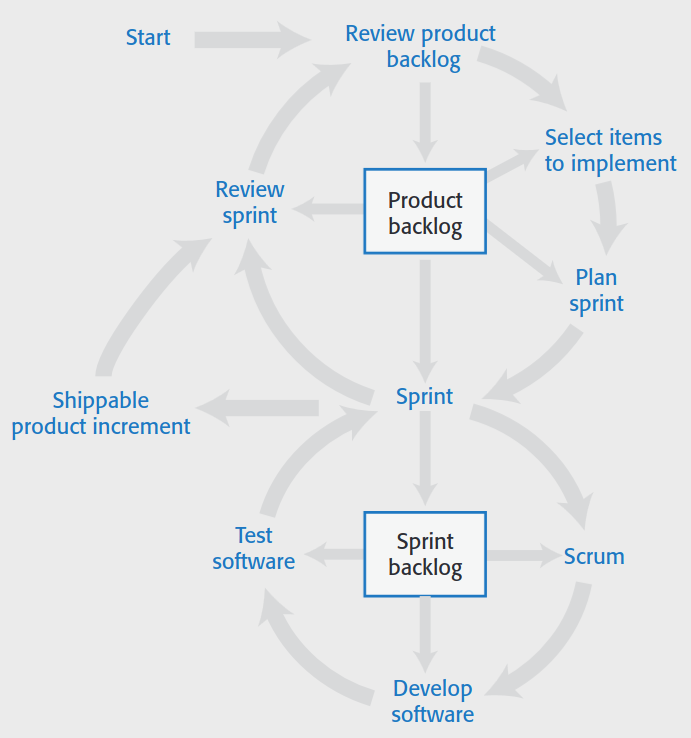
\includegraphics[width=0.7\textwidth]{images/Agile/ScrumCycle.png}
    \caption{Sprint activities within the Scrum cycle}
    \label{fig:scrumcycle}
\end{figure} 

\subsubsection{Sprint Planning}

Sprint planning involves establishing an agreed sprint goal, which may focus on software functionality, support, performance, or reliability. To define the goal, the team selects which items from the product backlog should be implemented. The outcome of this process is a \textbf{sprint backlog}, a more detailed version of the product backlog, listing the tasks to be completed during the sprint. \\

Throughout the sprint, the team holds \textbf{daily Scrum meetings} to coordinate their work. These meetings, often called \emph{scrums}, are short and typically held at the beginning of the day. During the meeting, each team member shares their progress, any problems encountered, and their plans for the day. This ensures that everyone on the team knows what is happening and allows for quick re-planning if needed. Scrum meetings should remain short and focused. To avoid prolonged discussions, they are sometimes held as ‘stand-up’ meetings, where no chairs are provided. \\

During a Scrum, the sprint backlog is reviewed, completed items are removed, and new items may be added as new information arises. The team then decides which team member will work on specific sprint backlog items for the day.

\subsubsection{Sprint Execution}

Scrum does not prescribe specific technical agile activities to be used during a sprint, but two practices are commonly recommended by agile software engineers:

\begin{itemize}
    \item \textbf{Test Automation}: As much testing as possible should be automated. A suite of executable tests should be developed, which can be run at any time to ensure software quality.
    \item \textbf{Continuous Integration}: Whenever changes are made to software components, they should be immediately integrated with the other components to form a complete system. This system should then be tested to check for any unanticipated issues from component interactions.
\end{itemize}

\subsubsection{Sprint Review}

At the end of each sprint, the team conducts a sprint review meeting, involving all team members. The meeting reviews whether the sprint goal was met, addresses any new issues that arose during the sprint, and provides a chance for the team to reflect on how to improve their work process. \\

The product owner has the authority to decide whether the sprint goal has been achieved. They confirm whether the implementation of the selected product backlog items is complete. Additionally, the sprint review should include a process review where the team reflects on how they’ve used Scrum and discusses how to improve productivity in the next sprint.

\subsection{Execution}

Depending on the state of the item, there are different possible actions:

\begin{itemize}
	\item \textbf{Refinement}: Existing PBIs are analyzed and refined to create more detailed PBIs. This may lead to the creation of new product backlog items.
	\item \textbf{Estimation}: The team estimates the amount of work required to implement a PBI and adds this assessment to each analyzed PBI.
	\item \textbf{Creation}: New items are added to the backlog. These may include new features suggested by the product manager, required feature changes, engineering improvements, or process activities such as assessing development tools that might be used.
    \item \textbf{Prioritization}: New items are prioritized within the backlog. These may also include new features suggested by the product manager, required feature changes, engineering improvements, or process activities such as assessing development tools that might be used.
\end{itemize}

We can see the effects of these actions in Figure \ref{fig:productbacklog}. There are metrics that we can apply to PBIs in order to choose the next state or action. The following factors are usually considered:

\begin{itemize}
\item \textbf{Effort required}: This may be expressed in person-hours or person-days, i.e., the number of hours or days it would take one person to implement that PBI. This is not the same as calendar time, as several people may work on an item, which can shorten the calendar time required.
\item \textbf{Story points}: Story points are an arbitrary estimate of the effort involved in implementing a PBI, taking into account the size of the task, its complexity, the technology that may be required, and the ‘unknown’ characteristics of the work. They were originally derived by comparing user stories but can be used for estimating any kind of PBI. Story points are estimated relatively; the team agrees on the story points for a baseline task, and other tasks are estimated by comparison with this, e.g., more/less complex, larger/smaller, etc.
\end{itemize}


\chapter{Features, Scenarios, and Stories}

These are the factors that drive the design of software products:
\begin{itemize}
    \item Inspiration
    \item Business/consumer needs not met by existing products
    \item Dissatisfaction with existing products
    \item Technical changes making new product types possible
\end{itemize}

We'll understand how to reach the specification of the software product we want to create. We saw that discussing requirements with the client is usually hard, mostly because of the language barrier and the fact that most clients don't even know which functionalities they want. \\

We observed that product-based software engineering requires less documentation than project-based software engineering. In Agile, requirements are not set by customers and change often. That's why developers need to identify product features: they must understand potential users and how to attract them (through interviews, surveys, informal consultations, and so on).

User representations (\textbf{personas}) and natural language descriptions (\textbf{scenarios and stories}) help identify product \textbf{features}. 

\begin{figure} [H]
    \centering
    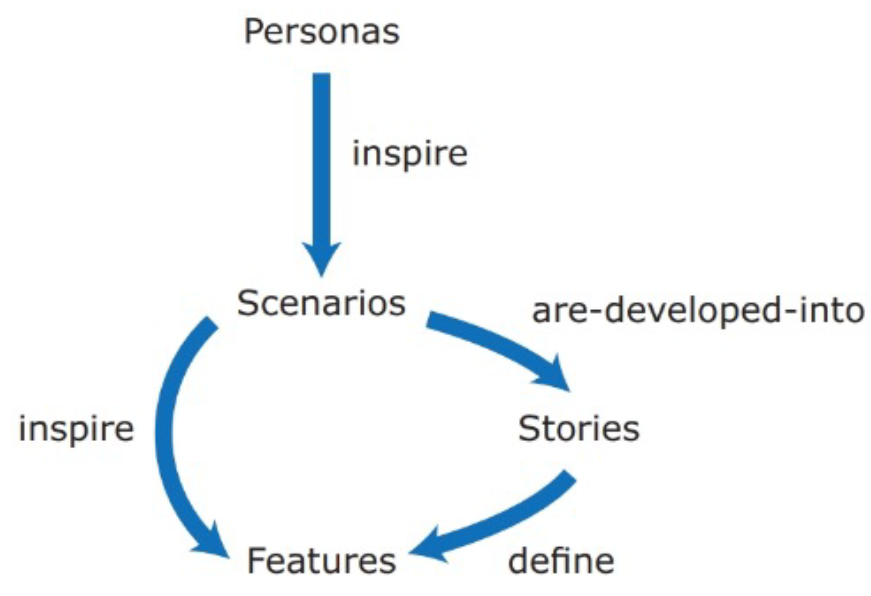
\includegraphics[width=0.48\textwidth]{images/Stories/scenariostories.png}
    \caption{Features generation process}
    \label{fig:scenariostories}
\end{figure} 

\section{Personas}

Personas are the target users for our product. Programmers need to understand potential users to design features that are useful for them. The background, skills, and experience of potential users are important because these factors will influence the user experience and the user interface. Generally, only a few (1-2, max 5) personas are required to identify key product features. Personas allow developers to “step into the users' shoes.” \\

\noindent Let's examine the key features of personas:

\begin{itemize}
    \item \textbf{Personalization}: You should give them a name and describe their personal circumstances. It is sometimes helpful to use an appropriate stock photograph to represent the person in the persona. Some studies suggest that this helps project teams use personas more effectively.
    \item \textbf{Job-related}: If your product is targeted at businesses, you should describe their job and (if necessary) what the job involves. For some jobs, such as teaching, where readers are likely familiar with the role, this may not be necessary.
    \item \textbf{Relevance}: If possible, you should explain why they might be interested in using the product and what they might want to do with it.
    \item \textbf{Education}: You should describe their educational background and their level of technical skills and experience. This is important, especially for interface design.
\end{itemize}

\begin{figure} [H]
    \centering
    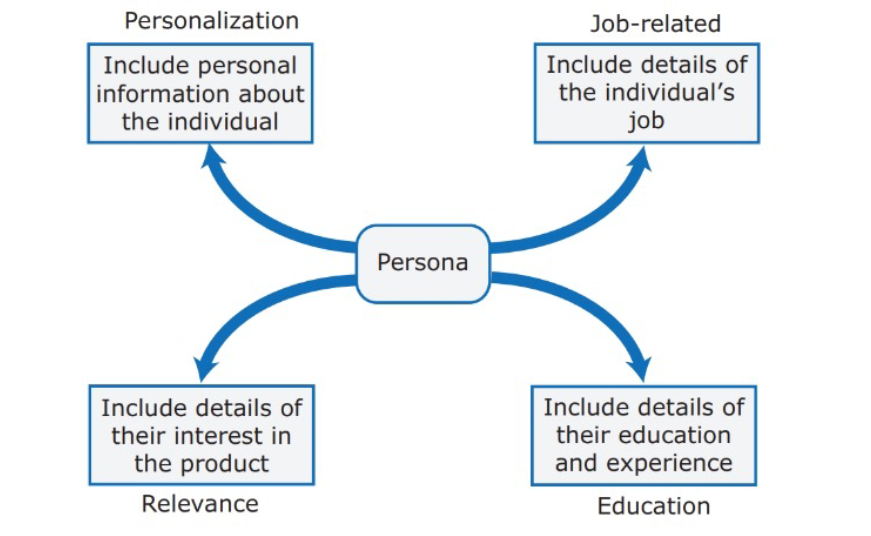
\includegraphics[width=0.8\textwidth]{images/Stories/personadescription.png}
    \caption{Personas' key features}
    \label{fig:personadescription}
\end{figure} 

Some developers also use an appropriate stock photograph to represent the person in the persona. Studies have shown that we have biases depending on the photo, so not everyone accepts the use of pictures. When studying users is not possible (e.g., for some new products), we can develop proto-personas: these are imagined personas.

\section{Scenarios}

Once the personas are created, the next step is to work with scenarios. To discover product features, we can define \textbf{scenarios} of user interactions with the product. A scenario is a narrative describing a situation in which a user is using our product’s features to accomplish a specific goal. \\

Let's examine the key features of scenarios:

\begin{figure} [H]
    \centering
    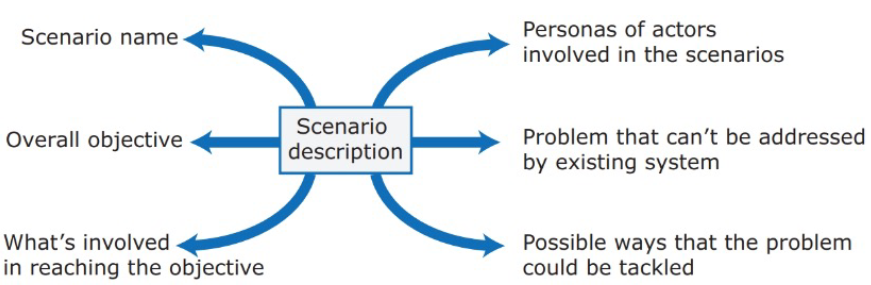
\includegraphics[width=0.8\textwidth]{images/Stories/scenariodescription.png}
    \caption{Scenario's key features}
    \label{fig:scenariodescription}
\end{figure} 

Narrative, high-level scenarios facilitate communication and stimulate design creativity. Scenarios are not specifications, though; they lack details and may be incomplete. Usually, several scenarios (e.g., 3-4) are required for each persona, covering the main responsibilities of the persona. The scenarios are written from the \emph{user’s perspective}. Each team member should individually create some scenarios, then discuss them with the rest of the team and, if possible, with users.

\section{User Stories}

Scenarios are high-level stories of product use, while user stories are finer-grained narratives. They follow a structure, which is as follows: 

As a \textit{<role>} I want to \textit{<do something>} so that \textit{<reason/values>}.

\newpage

User stories are not part of the Agile manifesto, but they help to adhere to Agile principles: 
\newline \noindent - Our highest priority is to satisfy the customer through early and continuous delivery of valuable software.
\newline \noindent - Working software is the primary measure of progress.
\newline \noindent - Simplicity, the art of maximizing the amount of work not done, is essential. \\

User stories also help visualize the progress made in our program. We can write the short stories on sticky notes to stick them on a to-do board. We need to remember that \emph{stories that don't create business value for the customer are work that isn't going to count as progress. Additionally, creating stories that depend on one another might create deadlocks}. \\

The Scrum product backlog is often a set of user stories. Long stories (\emph{epics}) must be broken into simpler stories. Stories are associated with \textbf{priorities} (and possibly also with an estimate of effort needed to implement the story) and sorted according to priority (\emph{requirements triage}). It is possible to express all the functionalities described in a scenario as user stories, but scenarios read more naturally, making it easier to understand stories and providing more context (we can sell stories to stakeholders).

The final goal of the user stories is to identify the features that define our product. These features should, in principle, have the following properties:

\begin{itemize}
    \item \textbf{Independence}: A feature should not depend on how other system features are implemented and should not be affected by the order of activation of other features.
    \item \textbf{Coherence}: Features should be linked to a single item of functionality. They should not do more than one thing and should never have side effects.
    \item \textbf{Relevance}: System features should reflect the way users normally carry out some tasks. They should not offer obscure functionality that is rarely required.
\end{itemize}
\newpage
The knowledge required for feature design is:

\begin{figure} [H]
    \centering
    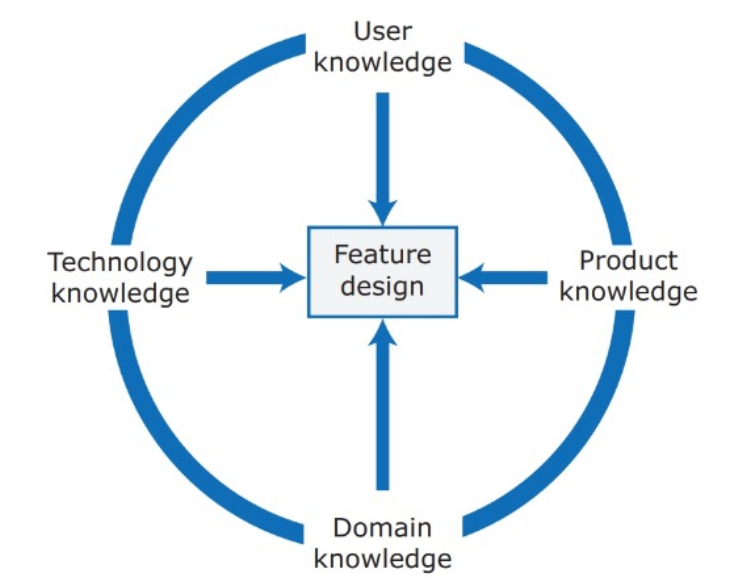
\includegraphics[width=0.6\textwidth]{images/Stories/feature_design.png}
    \caption{Feature design knowledge required}
    \label{fig:featuredesign}
\end{figure} 

\begin{itemize}
    \item \textbf{User Knowledge}: You can use user scenarios and user stories to inform the team of what users want and how they might use the software features.
    \item \textbf{Product Knowledge}: You may have experience with existing products or decide to research what these products do as part of your development process. Sometimes your features have to replicate existing features in these products because they provide fundamental functionality that is always required.
    \item \textbf{Domain Knowledge}: This is knowledge of the domain or work area (e.g., finance, event booking) that your product aims to support. By understanding the domain, you can think of new innovative ways of helping users accomplish their goals.
    \item \textbf{Technology Knowledge}: New products often emerge to take advantage of technological developments since their competitors were launched. If you understand the latest technology, you can design features to make use of it.
\end{itemize}

\newpage
It's important to find a balance between opposing factors in feature design.

\begin{figure} [H]
    \centering
    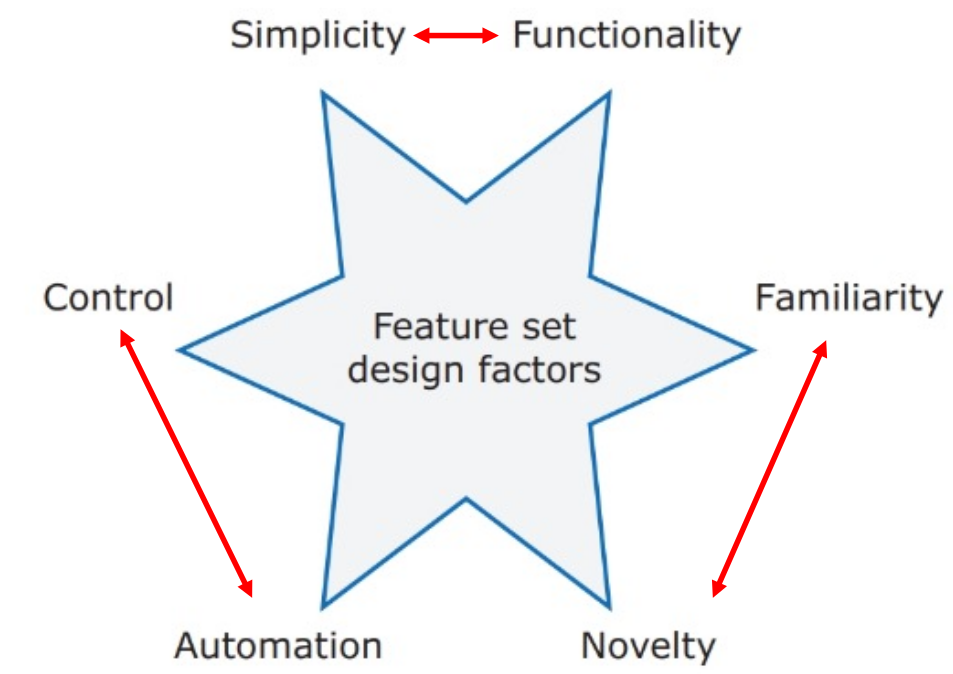
\includegraphics[width=0.6\textwidth]{images/Stories/factors_design.png}
    \caption{Factors in feature design}
    \label{fig:factorsdesign}
\end{figure}

The number of product features grows as new potential users are envisaged (this is also known as \textbf{Feature Creep}). This growth is dictated by marketing executives who want to meet all users' demands. Marketing also pressures teams to include competitors' features and has the desire to support both experienced and inexperienced users. To avoid feature creep, making feature questions usually allows understanding which features are pointless.

\begin{figure} [H]
    \centering
    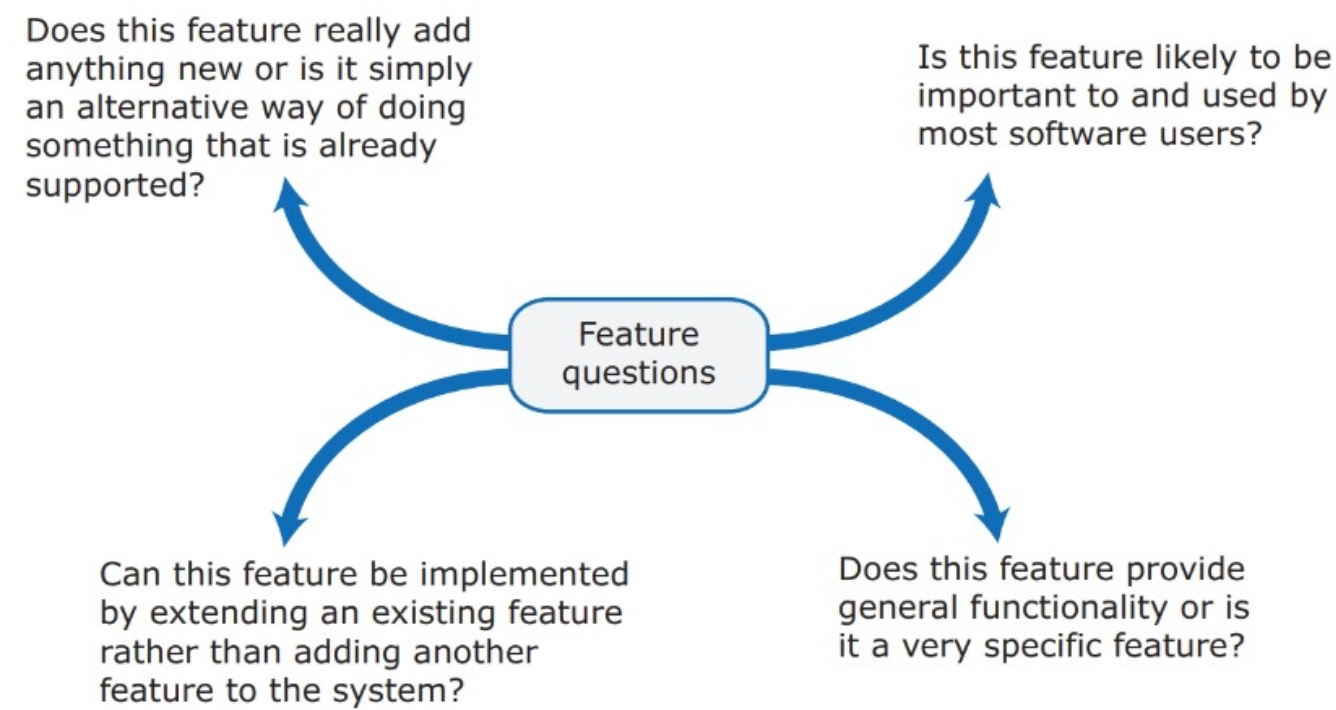
\includegraphics[width=0.9\textwidth]{images/Stories/feature_creep.png}
    \caption{Feature questions to avoid feature creep}
    \label{fig:featurecreep}
\end{figure}
\newpage

The product development team must meet to discuss scenarios and stories to extract the list of product feature descriptions. This consists of detecting the input and activation for the action required in the feature and then writing the expected output for the action.

\begin{figure} [H]
    \centering
    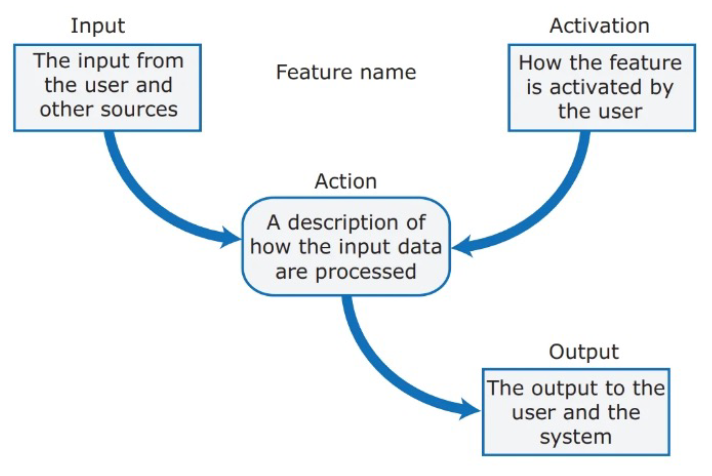
\includegraphics[width=0.8\textwidth]{images/Stories/Feature_derivation.png}
    \caption{Feature derivation}
    \label{fig:featurederivation}
\end{figure}


\chapter{Software Architecture}

Architecture is the fundamental organization of a software system, embodied in its components, their relationships to each other and to the environment, and the principles guiding its design. The software architecture affects \emph{performance, usability, security, reliability, maintainability}, and so on.

Architecture is made up of \textbf{components}, where components implement a coherent set of \textbf{features} (services that may be used by other components). Here's an example of component usage:

\begin{figure} [H]
    \centering
    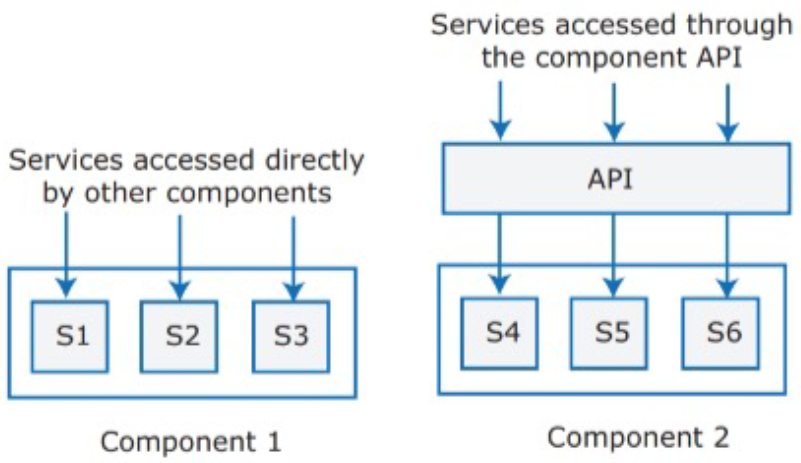
\includegraphics[width=0.7\textwidth]{images/SoftwareArchitecture/componentAPI.png}
    \caption{API to call component services}
    \label{fig:componentAPI}
\end{figure} 

In all cases where the software is large, developers will need to develop \textbf{APIs} (Application Programming Interfaces) to allow communication between components that might even be implemented with different technologies. \\

When we design our software, we need to take into account different aspects. These are some issues that are usually addressed:

\begin{itemize}
    \item \textbf{Non-functional product characteristics}: Non-functional product characteristics such as security and performance affect all users. If you get these wrong, your product is unlikely to be a commercial success. All these characteristics have a cost (e.g., availability, security, and so on).
    \item \textbf{Product lifetime}: If you anticipate a long product lifetime, you need to create regular product revisions. You therefore need an architecture that can evolve, so that it can be adapted to accommodate new features and technologies.
    \item \textbf{Software reuse}: You can save a lot of time and effort if you reuse large components from other products or open-source software. However, this constrains your architectural choices because you must fit your design around the software that is being reused.
    \item \textbf{Number of users}: If you are developing consumer software delivered over the internet, the number of users can change very quickly. This can lead to serious performance degradation unless you design your architecture so that your system can be quickly scaled up and down.
    \item \textbf{Software compatibility}: For some products, it is important to maintain compatibility with other software so that users can adopt your product and use data prepared using a different system. This may limit architectural choices, such as the database software that you can use.
\end{itemize}

\section{Non-functional Quality Attributes}

When we talk about \textbf{non-functional product characteristics}, we are defining a set of specifications that describe the system’s operational capabilities and constraints and attempt to improve its functionality. This is a list of the most popular ones:

\begin{itemize}
    \item \textbf{Responsiveness}: Does the system return results to users in a reasonable time? 
    \item \textbf{Reliability}: Do the system features behave as expected by both developers and users? 
    \item \textbf{Availability}: Can the system deliver its services when requested by users?
    \item \textbf{Security}: Does the system protect itself and users' data from unauthorized attacks and intrusions?
    \item \textbf{Usability}: Can system users access the features they need and use them quickly and without errors? 
    \item \textbf{Maintainability}: Can the system be readily updated and have new features added without undue costs?
    \item \textbf{Resilience}: Can the system continue to deliver user services in the event of partial feature failure or an external attack?
\end{itemize}

For each non-functional quality attribute we implement, we also need to test them. This increases the product cost. 
Usually, optimizing one non-functional attribute affects others (e.g., to achieve more security with longer keys, we may need to sacrifice some performance or usability).

The prototypes don't need to respect these characteristics because we want to quickly build a prototype. \\

\emph{Good practice} for maintainability is to decompose the system into small, self-contained parts and avoid shared data structures. Not having centralized data structures is a good practice because if one component needs to change the database organization, this does not affect the other components. The system can also continue to provide partial service in the event of a database failure.

\begin{figure} [H]
    \centering
    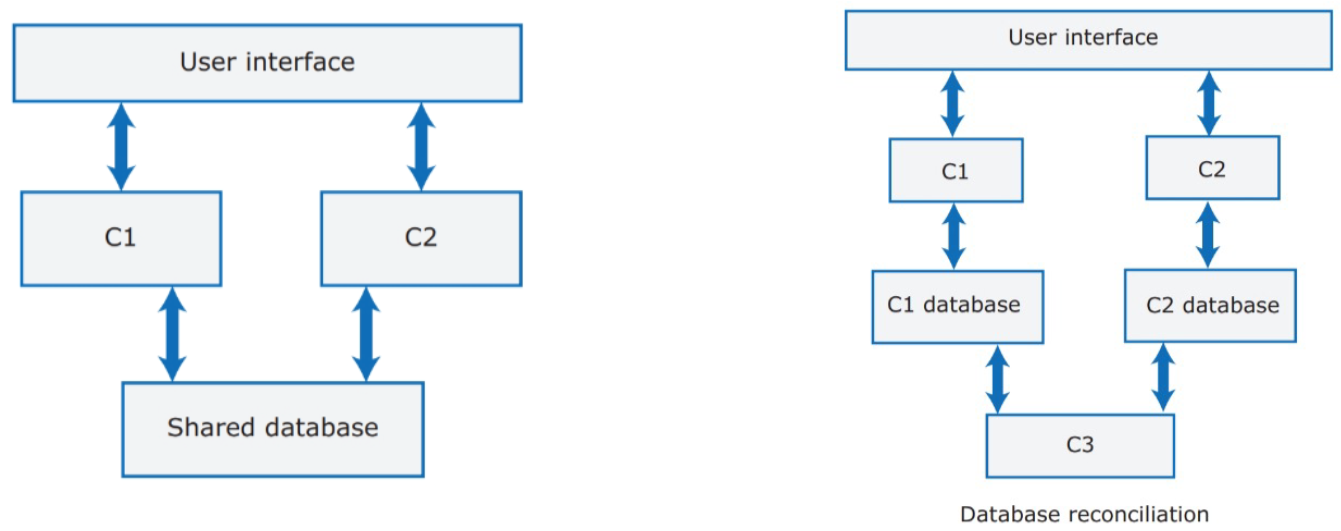
\includegraphics[width=0.9\textwidth]{images/SoftwareArchitecture/shattedDB.png}
    \caption{Database partitioning}
    \label{fig:shattedDB}
\end{figure} 

The cost of this practice is \emph{eventual consistency}: if component C1 makes a change (see Figure \ref{fig:shattedDB}), sooner or later that change must be reported to the C3 database. This is an additional cost. This also applies in the case of availability: if you want more availability, you can deploy multiple databases, but this requires synchronizing multiple databases. When something goes wrong in a distributed system, it's hard to roll back transactions. That's why we usually give up on consistency in order to achieve availability.

\newpage

\section{System Decomposition}

As we already said, a \emph{service} is a coherent unit of functionality, a \emph{component} is a software unit offering one or more services, and a \emph{module} is a set of components.

\begin{figure} [H]
    \centering
    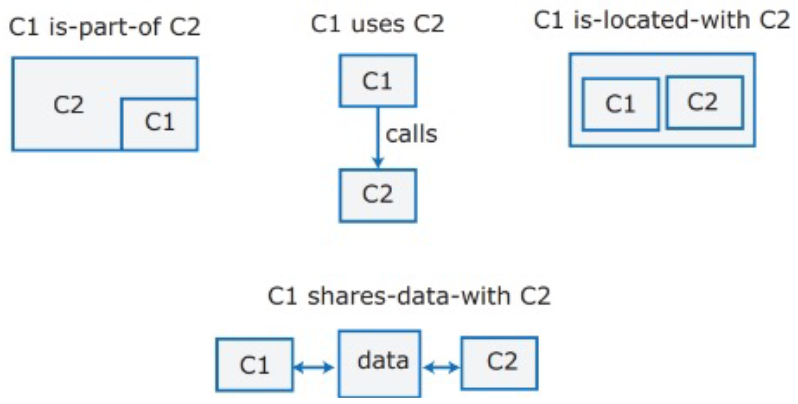
\includegraphics[width=0.7\textwidth]{images/SoftwareArchitecture/componentrelationship.png}
    \caption{Example of component relationships}
    \label{fig:componentrelationship}
\end{figure} 

As the number of components increases, the number of relationships tends to increase at a faster rate. Therefore, we should \textbf{decompose} as much as needed. The reason we want to decompose is to have simpler parts that can be maintained separately. In order to decompose a system, one good idea is \emph{separation of concerns}, as we will see with microservices that implement one business feature. We also want to have \emph{stable interfaces}, unless this is really necessary. The dogma of \emph{implement once} contrasts with the idea of independent teams that work with independent systems, but there aren't fixed rules; we always need to find trade-offs.

\begin{figure} [H]
    \centering
    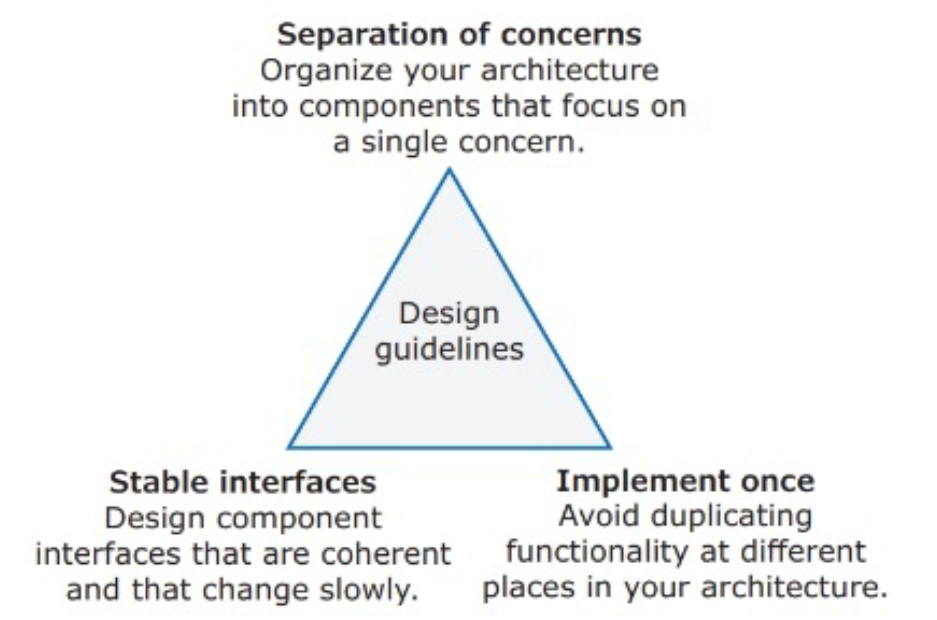
\includegraphics[width=0.7\textwidth]{images/SoftwareArchitecture/designguidelines.png}
    \caption{Design guidelines to control complexity}
    \label{fig:designguidelines}
\end{figure}

\newpage

Another aspect of system decomposition is having a \textbf{layered architecture}. Each layer is an area of concern and is considered separately from other layers. Within each layer, the components are independent and do not overlap in functionality. The architectural model is a high-level model that doesn't include implementation information. Software architects usually customize \emph{generic layers} by adding or removing layers until the architecture achieves a good form for its goals.

\begin{figure} [H]
    \centering
    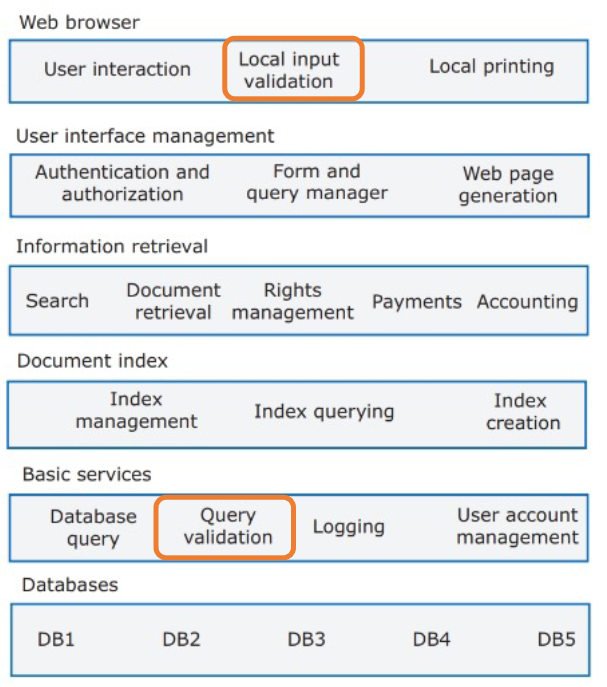
\includegraphics[width=0.7\textwidth]{images/SoftwareArchitecture/layaredarchitecture.png}
    \caption{Example of a layered architecture}
    \label{fig:layaredarchitecture}
\end{figure}

There are some systemic concerns that affect the whole system, so every layer must take them into account. \textbf{Cross-cutting concerns} (such as \emph{security, performance, reliability, validation}, and so on) add interactions between the layers. In the example shown in Figure \ref{fig:layaredarchitecture}, we can see that validation is considered in multiple layers. \\

On one hand, when we design architecture, we don't want to discuss implementation (because we don't want to limit the design with implementation details), but at the same time we need to consider possible implementations to understand how to design the architecture (e.g., the choice of using a relational database affects components at higher layers).

\section{Distribution Architecture}

The \textbf{distribution architecture} defines servers and the allocation of components to servers, specifying where the software will be deployed and run during production. \\

The most common type is the \textbf{client-server architecture}, which is suited for applications in which clients access a shared database and perform business logic operations on that data. Clients interact with \emph{load balancers} in the system, which are deployed on a cluster of servers.

\begin{figure} [H]
    \centering
    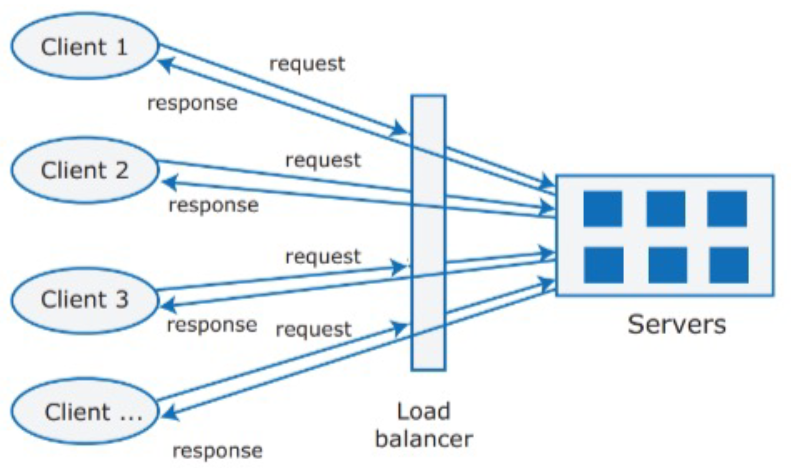
\includegraphics[width=0.7\textwidth]{images/SoftwareArchitecture/clientserverarchitecture.png}
    \caption{Example of a client-server architecture}
    \label{fig:clientserverarchitecture}
\end{figure}

\begin{wrapfigure}{r}{0.5\textwidth}
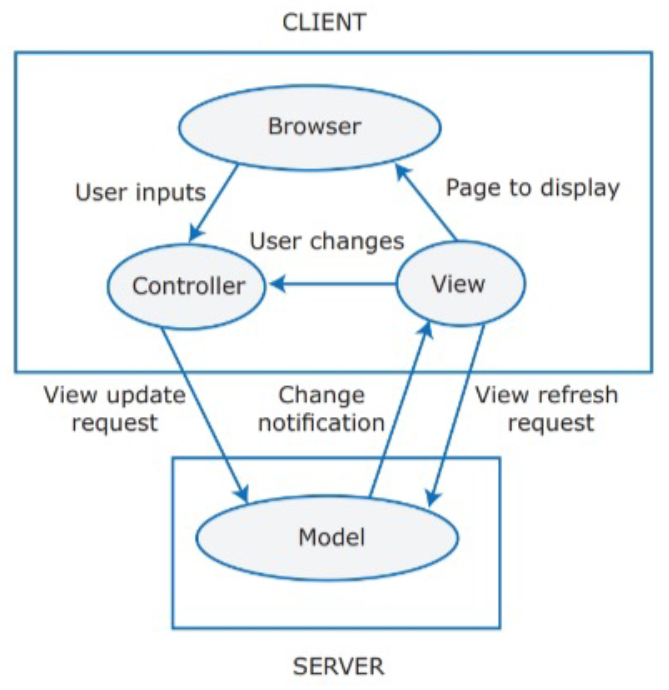
\includegraphics[width=0.45\textwidth]{images/SoftwareArchitecture/MVC.png}
    \caption{Model-View-Controller}
    \label{fig:MVC}
\end{wrapfigure}

\vspace{0.5cm}
\textbf{Model-View-Controller} is a widely used \emph{pattern}. This pattern helps to structure the code by dividing it into the \textit{Model part}, the \textit{View part}, and the \textit{Controller part}. In many cases, this also helps to understand how to implement the communications between the parts, which affects the simplicity and efficiency of the architecture (in many cases, the communication is implemented with HTTP + JSON). 

The pattern shown in Figure \ref{fig:MVC} is able to separate the logic of data presentation from business logic. This pattern is positioned at the logical or business level and is presented in a multi-tier architecture.

\newpage

\begin{figure} [H]
    \centering
    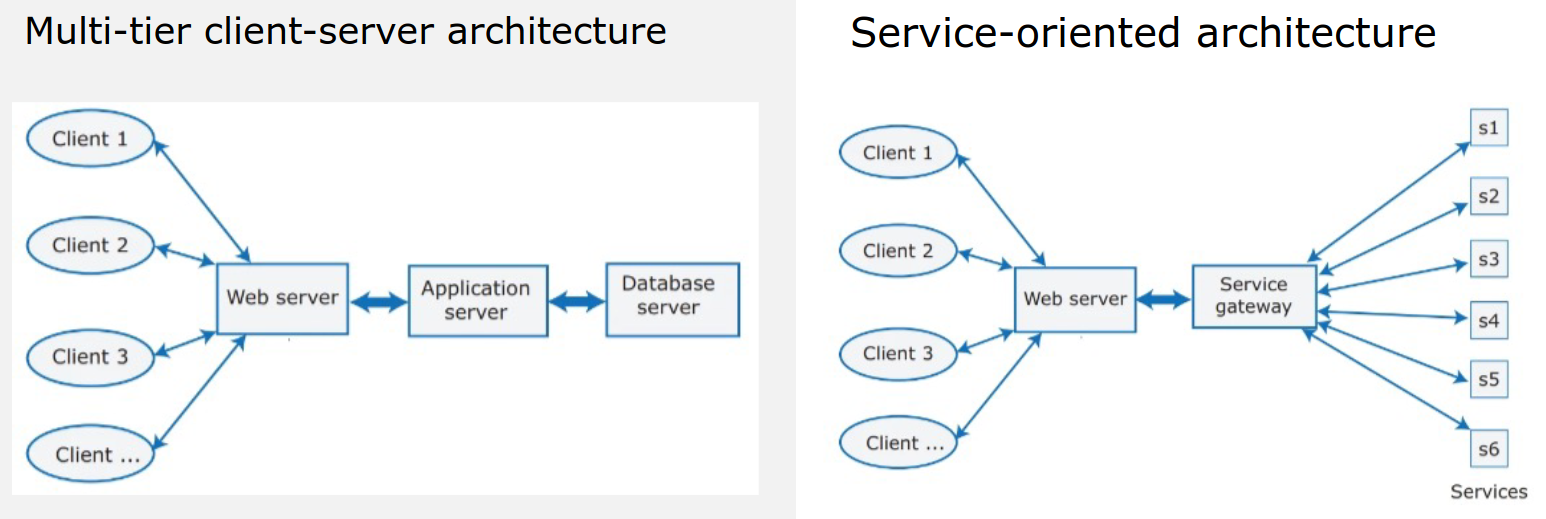
\includegraphics[width=1\textwidth]{images/SoftwareArchitecture/architectures.png}
    \caption{Common types of client-server architecture}
    \label{fig:architectures}
\end{figure}

Client-server architectures can be implemented in different ways (as shown in Figure \ref{fig:architectures}). The \textit{Service-oriented architecture} is slightly different: it has a Service gateway which splits the service requests to the appropriate service.
\newline\noindent
The choice of distribution architecture depends on several factors:
\begin{itemize}
    \item \textbf{Data type and data updates}: If you are mostly using structured data that may be updated by different system features, it is usually best to have a single shared database that provides locking and transaction management. If data is distributed across services, you need a way to keep it consistent, and this adds overhead to your system.
    \item \textbf{The system execution platform}: If you plan to run your system on the cloud with users accessing it over the Internet, it is usually best to implement it as a service-oriented architecture because scaling the system is simpler. If your product is a business system that runs on local servers, a multi-tier architecture may be more appropriate.
    \item \textbf{Change frequency}: If you anticipate that system components will be regularly changed or replaced, then isolating these components (inside containers) as separate services simplifies those changes.
\end{itemize}

\section{Technology Choices}

There are several ``relevant'' technology choices. These are considered relevant because changes in product design will reflect on these technologies, resulting in increased complexity and costs required to modify them during development.

\newpage
\noindent
This is a list of some relevant technologies:
\begin{itemize}
    \item \textbf{Database}: You should use either a \textit{relational SQL database} (where data is organized into structured tables, particularly suitable when transaction management is needed and data structures are predictable and simple) or an \textit{unstructured NoSQL database} (where data has a more flexible, user-defined organization. This option is more efficient for data analysis, and data can be organized hierarchically. It also supports efficient concurrent processing of 'big data').
    \item \textbf{Delivery Platform}: This refers to the platform where the product will ultimately run. Delivery can be web-based or mobile, but each platform presents its own challenges (e.g., mobile device issues include intermittent connectivity, processor power, power management, reduced screen size, and on-screen keyboard). It's advisable to decide on the platform early in order to begin the development phase as soon as possible.
    \item \textbf{Server}: Will the product run in a public cloud, or will it use in-house servers? Most consumer products utilize a set of microservices, which are containerized and deployed in the cloud (with their Service-Oriented Architecture, SOA). In contrast, business products are more concerned with cloud security issues (e.g., where and how client data will be stored). Once it's decided that the product will be launched in the cloud, the next decision is to choose a provider (note that it can be challenging to migrate a product across cloud providers due to vendor lock-in).
    \item \textbf{Open Source}: Are there suitable open-source components that could be incorporated into the product? Are these open-source components secure enough?
    \item \textbf{Development Tools}: Development technologies (e.g., mobile development toolkits, web application frameworks) influence the architecture of your product. The development technology that developers are familiar with may indirectly affect the architecture of the product.
\end{itemize}

\section{Enterprise Application Integration}

\textbf{Enterprise applications} are large software systems typically designed to operate in a corporate environment, such as business or government. These applications are extensive systems where users can typically only see the front-end, while a lot of backend functionality (made up of multiple services) supports it. The various heterogeneous services can be classified as \emph{sources} (services that only make requests), \emph{sinks} (services that only respond to requests), or a mix of both categories. These services communicate using various \emph{heterogeneous data types} (with different representations, even for analogous data), and this information can be shared with \emph{different organizations} over the \emph{network}. This complexity makes enterprise applications distributed multi-service applications whose services must work together and be suitably integrated.

The architectural question is how to integrate all of this in a coherent, extensible, and maintainable way. There is a need to manage these complexities, and one approach is to use \textbf{patterns}. A pattern is a high-level abstraction of accepted, reusable solutions for recurring problems. Patterns are defined in terms of problem statements (what problem the pattern solves), context (there may be different patterns for the same problem), forces (why you should consider using a pattern for the problem), and solutions (how to apply the pattern to solve the problem). The idea of patterns is to avoid reinventing the wheel and instead use established patterns. \textbf{Enterprise Application Integration} (EAI) is a reusable abstraction of proven solutions to well-known problems that arise while integrating the software components and services forming enterprise applications. 

\subsection{Patterns}

These patterns were studied more than 20 years ago. Among all the patterns, the most commonly used are \textbf{messaging patterns}, as shown in Figure \ref{fig:EIPpatterns}.

\begin{figure} [H]
    \centering
    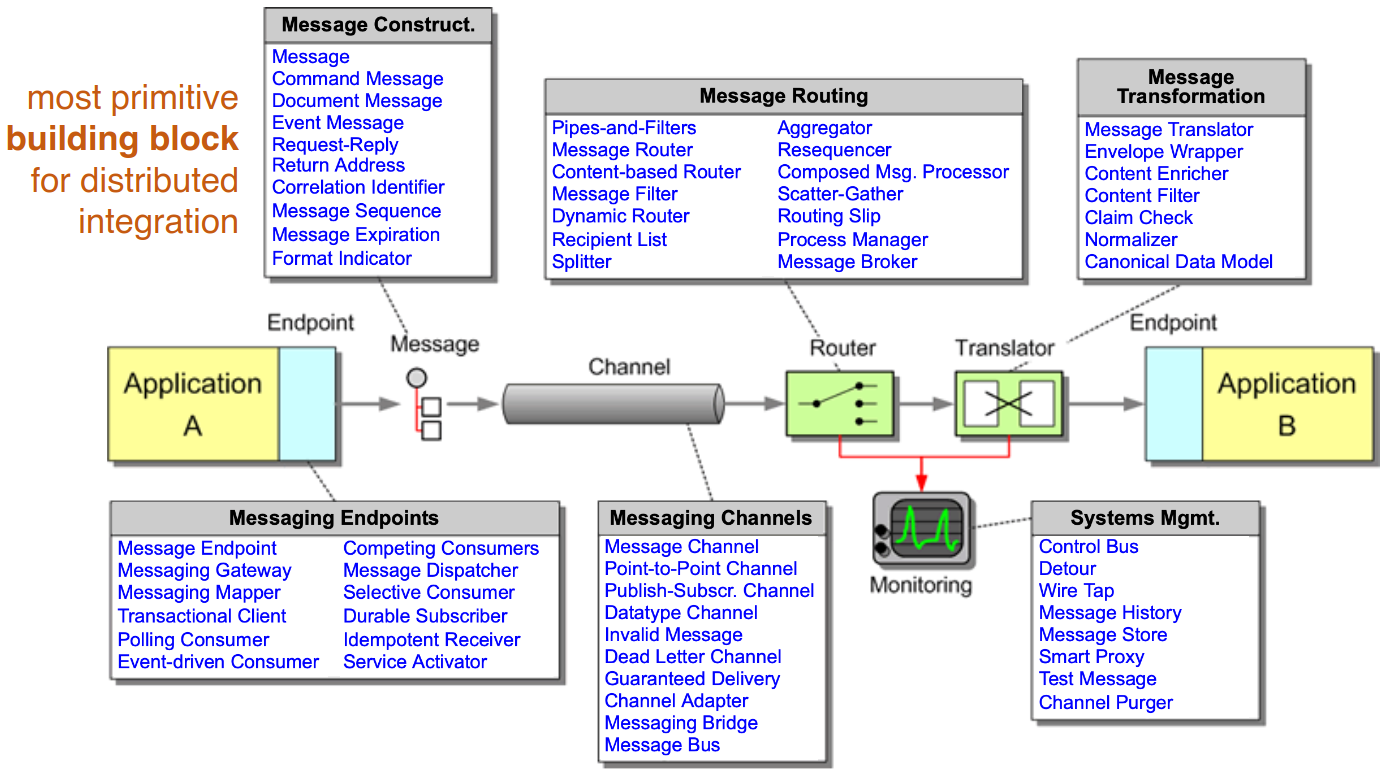
\includegraphics[width=1\textwidth]{images/SoftwareArchitecture/EIPpatterns.png}
    \caption[Caption for EAI messaging patterns]{Messaging Patterns\protect\footnotemark}
    \label{fig:EIPpatterns}
\end{figure}
\footnotetext{\url{https://www.enterpriseintegrationpatterns.com/patterns/messaging/}}

A message is a discrete piece of data sent from one service to another. Typically, messages are structured into a \textit{header} (metadata) and a \textit{body} (payload). Concrete examples of messages include \emph{document messages} (pure data), \emph{event messages} (notifications of events), and \emph{command messages} (commands sent to perform actions).

\begin{figure} [H]
    \centering
    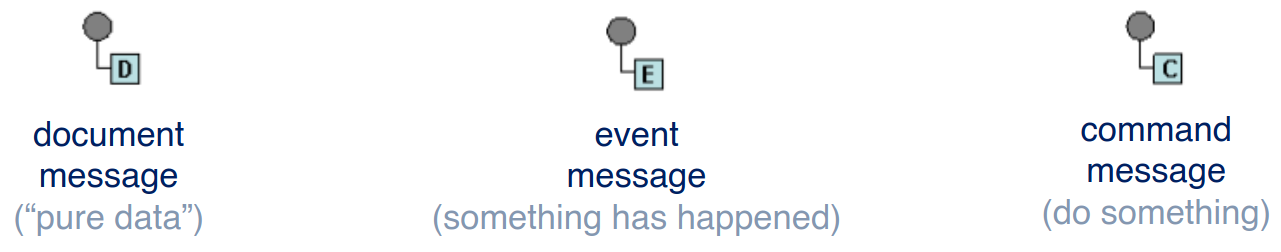
\includegraphics[width=1\textwidth]{images/SoftwareArchitecture/AEImessages.png}
    \caption{Example of concrete messages}
    \label{fig:AEImessages}
\end{figure}

The exchange of messages means that the services are not tightly connected but can communicate through messages. Message-based communication enables \emph{loose coupling}, and it is realized through \textbf{channels}: abstractions for components sending messages from a source to a destination (implemented in various ways, such as RPC, HTTP, TCP, and so on). Channels are \emph{one-way}, allowing communications to be natively asynchronous. Synchronous (request/response) communications use two channels. Application services are typically independent of the messaging systems; thus, \textbf{adapters} are used to enable application-specific data to be sent to channels. \textbf{Message endpoints} allow application services to send and receive messages to and from channels. There are different types of channels: the one shown in Figure \ref{fig:AEIsimpleintegration} is a \emph{point-to-point} channel (which ensures that only one receiver will receive a particular message), whereas another type is the \emph{publish-subscribe} channel (where the publisher delivers a copy of incoming messages to each subscriber).

\begin{figure} [H]
    \centering
    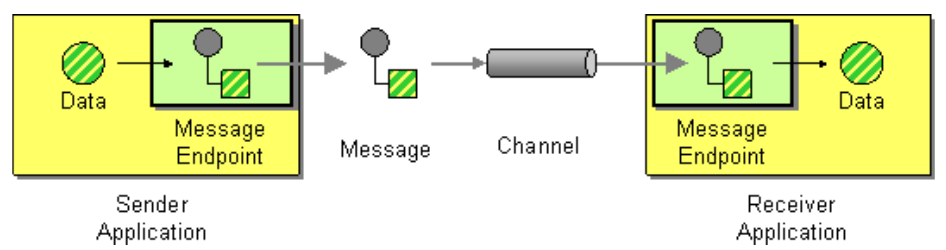
\includegraphics[width=1\textwidth]{images/SoftwareArchitecture/AEIsimpleintegration.png}
    \caption{Simple integration of message-based communication}
    \label{fig:AEIsimpleintegration}
\end{figure}

This implementation alone is not sufficient: what happens if the receiving service expects a different data format? A \textbf{message translator} allows the message to be adapted to suit the receiving services, but additional steps may still be necessary (e.g., how to route messages to different or multiple endpoints, how to split messages, and how to aggregate messages).

\newpage

\subsection{Pipes and Filters}

The \textbf{pipes and filters architectural style} (along with other EIPs) enables structuring the more complex integrations required by enterprise applications. Messages pass through multiple processing steps/components (the filters), while components send messages down the channels (pipes) to which they are connected. The idea is that messages flow through the pipes, and as they reach a filter, they may be transformed before reaching the sink (the target of the message). \\

One of the most common examples in the field of EAI is the \emph{Loan and Broker design}: the \emph{loan company} sends a request, the \emph{Credit Bureau} validates the request, the \emph{Rule Base} decides which office should process the request, and then the \emph{Banks} will be notified to accept or reject the loan. All the responses will be aggregated and sent back to the loan company. The shaded area in the Loan Broker example represents the Loan service.

\begin{figure} [H]
    \centering
    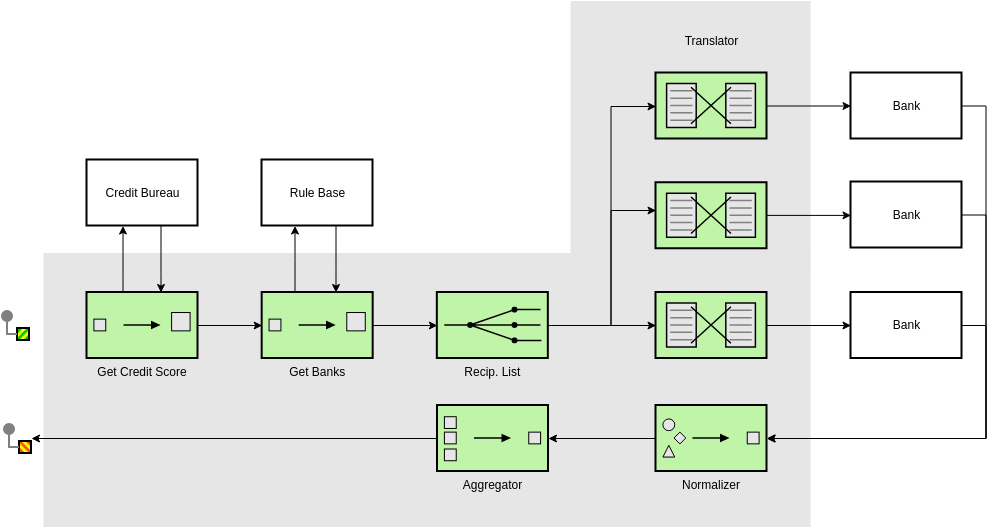
\includegraphics[width=1\textwidth]{images/SoftwareArchitecture/EAIloanbroken.png}
    \caption{Loan Broker Design}
    \label{fig:EAIloanbroken}
\end{figure}

This is a list of additional patterns used that haven't been described until now:

\begin{itemize}
    \item \textbf{Content Enricher}: This pattern uses information within the incoming message (e.g., key fields) to retrieve data from an external source. In the example shown in Figure \ref{fig:EAIloanbroken}, the calls \emph{Get Credit Score} and \emph{Get Banks} are examples of content enrichment. Retrieved data is appended to the message. Original information may either be retained or discarded.
    \item \textbf{Routers}: There are mainly two categories for message routing: \emph{content-based routers} route messages based on message type (in headers) or message content (in the body), while \emph{context-based routers} route based on contextual information retrieved from a central configuration location.
    
    In general, a message router connects to multiple channels and contains the logic to decide which channel it should send to.

    \begin{figure} [H]
        \centering
        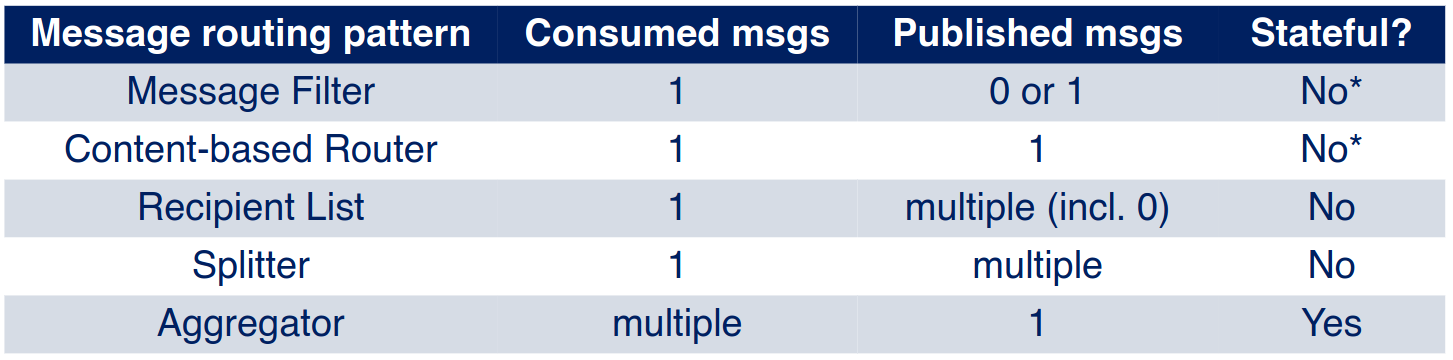
\includegraphics[width=1\textwidth]{images/SoftwareArchitecture/messageRoutingpattern.png}
        \caption{Message routing patterns}
        \label{fig:messageRoutingpattern}
    \end{figure}
    
    A \textbf{recipient list} inspects an incoming message, determines the list of desired recipients, and forwards the message to all channels associated with the recipients in the list. A \textbf{content-based router} enables routing each message to the correct recipient based on the message content.
    \item \textbf{Normalizer}: This pattern enables translating messages to match a common data format. This is usually realized as a composition of multiple patterns: it is possible to combine several patterns to create \emph{composite patterns} (as is the case with the normalizer).
    
    \begin{figure} [H]
        \centering
        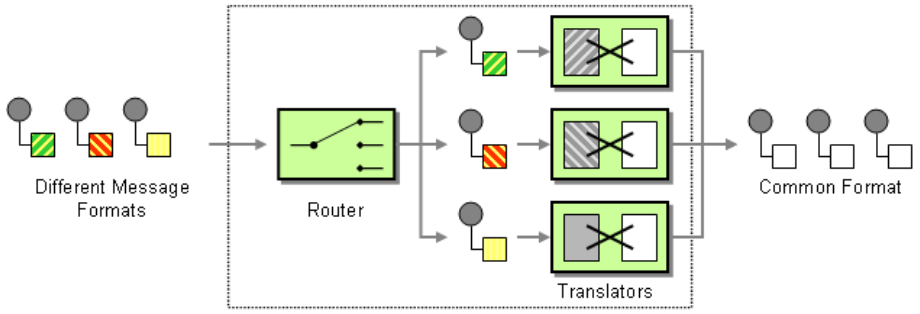
\includegraphics[width=0.9\textwidth]{images/SoftwareArchitecture/normalizer.png}
        \caption{Normalizer schema}
        \label{fig:normalizer}
    \end{figure}

    \item \textbf{Aggregator}: A (\emph{stateful}) aggregator collects and stores individual messages until a complete set of related messages has been received (see Figure \ref{fig:messageRoutingpattern} for reference). This is usually utilized when some integration steps may occur in parallel: independent processes can be executed in parallel, and the results of these processes can be aggregated to inform subsequent decisions on how to proceed.
\end{itemize}






\chapter{Cloud-based Software}

The revolution of cloud-based software began with the combination of two aspects: \emph{powerful computer hardware} and \emph{high-speed networking}, which have led to the development of cloud computing, and \emph{virtualized resources} (e.g., compute, storage, platform) accessible on demand.

The main advantages of cloud-based software are:
\begin{itemize}
    \item \textbf{Scalability}: Maintains performance as load increases (useful when developers do not know the number of the product's customers).
    \item \textbf{Elasticity}: Adapts server configuration to changing demands (we want to avoid \emph{underprovisioning} and \emph{overprovisioning}).
    \item \textbf{Resilience}: Maintains service in the event of server failures.
    \item \textbf{Cost}: Most cloud services are \emph{pay-per-use} (no need to buy hardware).
\end{itemize}

\section{Virtualization and Containers}

As mentioned before, one of the main aspects that led to cloud-based software is \emph{virtualized resources}. When we refer to \emph{compute power}, we mean servers and many other devices. It is possible to host many virtual servers inside the same physical server, which utilize virtual machines.

The left stack of Figure \ref{fig:virtualizedresources} refers to a machine with an \emph{OS} and a \emph{Hypervisor} (which enables virtualization; the one shown in the figure is a Level 2 Hypervisor, which depends on the OS. The Level 1 Hypervisor is bound to the hardware). The orange boxes are \textbf{virtual machines}, which are partitions of the physical machine.

The right stack consists of \textbf{containers}: rather than providing isolation (as it is with virtual machines), containers share the same OS to exploit the OS kernel’s capability of allowing multiple isolated user-space instances. Containers run on a \emph{container manager}, which operates on the OS. The advantage of OS sharing (which leads to much lighter and faster container startup) is counterbalanced by security issues (such as memory contamination from other containers).

\begin{figure}[H]
    \centering
    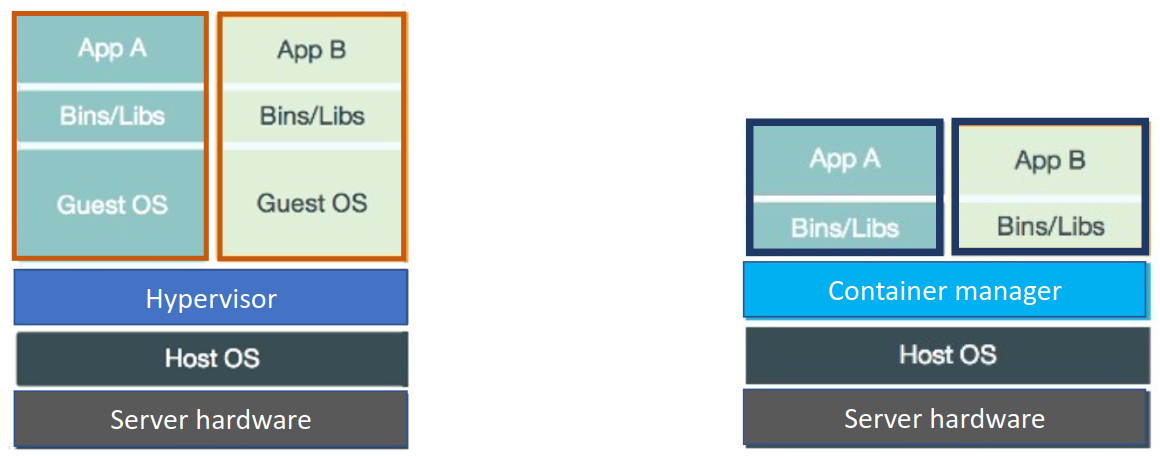
\includegraphics[width=0.8\textwidth]{images/Cloud/virtualizedresources.png}
    \caption{Virtual Machines and Containers}
    \label{fig:virtualizedresources}
\end{figure}

\subsection{Docker}

Portability of applications has been one of the biggest problems in software engineering: traditionally, there was one environment for developing and testing and another for production and distribution (the environment where the application was deployed and distributed to the user). These two environments were not the same, which meant that more time and money were required each time an application was moved between different environments.

\textbf{Docker} is a platform that allows us to run applications in an isolated environment. Docker enables the development and running of portable applications by utilizing containers: once an application is developed, it is encapsulated inside a container. When the container is opened in a new environment, it will not have portability issues, thanks to \textbf{Docker Engine} (used for creating and running containers). The \emph{Docker platform} also contains \textbf{Docker Hub}, which is used for distributing containers.

\begin{figure}[H]
    \centering
    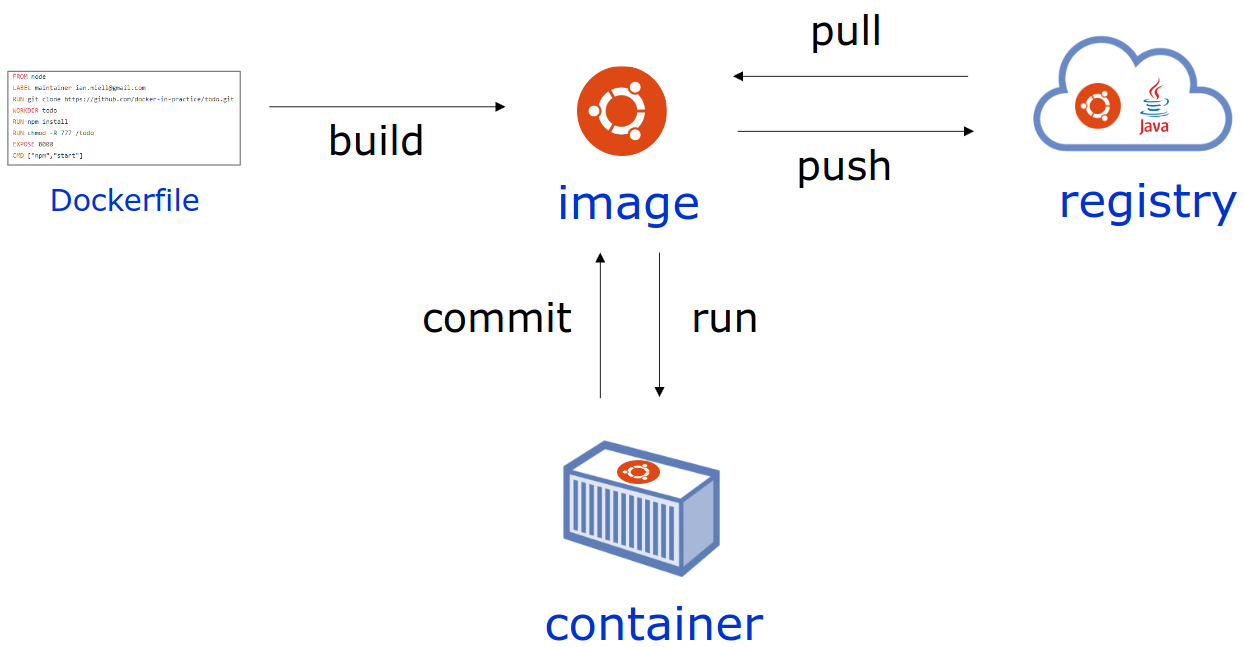
\includegraphics[width=0.8\textwidth]{images/Cloud/DockerCycle.png}
    \caption{Docker Life Cycle}
    \label{fig:DockerCycle}
\end{figure}

Software components are packaged into \textbf{images}, which are utilized as read-only templates to create and run \textbf{containers}. Since the templates are read-only, \emph{external volumes} are required to ensure data persistence. The images are stored in a (private or public) \textbf{Docker registry}: a registry structured in repositories, where each repository contains a set of images for different versions of software (images are identified by pairs repository:tag). Images are structured into layers, where each layer is in turn an image (the lowest layer is called the base image). \\

As we can see from Figure \ref{fig:DockerCycle}, the command \textbf{pull} retrieves an image from the \emph{registry}, while \textbf{push} uploads an image to the \emph{registry}. Images can be built from a \emph{Dockerfile} (see the documentation\footnote{\url{https://docs.docker.com/engine/reference/builder/}}) using the command \textbf{build}. Images can also be run in a \emph{container} using the command \textbf{run}. To modify the \emph{application} (and save a new version), the command \textbf{commit} must be used. \\

When an image generates multiple processes inside a container, the life of the container will be associated with the main process. It is good practice to create one container per process, so when the life of a process ends, it will not affect the other processes. In cases where the application consists of multiple services, Docker provides a tool called \textbf{Docker Compose} (see the documentation\footnote{\url{https://docs.docker.com/compose/}}), which not only allows running one container per service but also manages networking (it is possible to call the locally hosted services using their names) and communication between containers.

\section{Everything as a Service}

There are different deployment models of cloud computing:
\begin{itemize}
    \item \textbf{IaaS}: IaaS provides (virtualized) servers, storage, and networking. The IaaS provider manages all infrastructure. The client is responsible for all other aspects of the deployment (e.g., OS, application). Some examples include EC2 and S3.
    \item \textbf{PaaS} (Platform as a Service): PaaS provides a complete platform as a service (VMs, OS, services, SDKs, etc.). The PaaS provider manages infrastructure, OS, and enabling software. The client is responsible for installing and managing the application. Some examples include Heroku, Azure, and GAE.
    \item \textbf{SaaS} (Software as a Service): SaaS provides software on demand for use, accessible via thin clients or APIs. The SaaS provider manages infrastructure, OS, and application. The client is responsible for nothing, which is why this is the service with the largest market share. An example is Salesforce.com.
\end{itemize}

The following Figure \ref{fig:PizzaAsAService} represents an analogy of what each deployment model provides, and what clients need to manage on their own.

\begin{figure}[H]
    \centering
    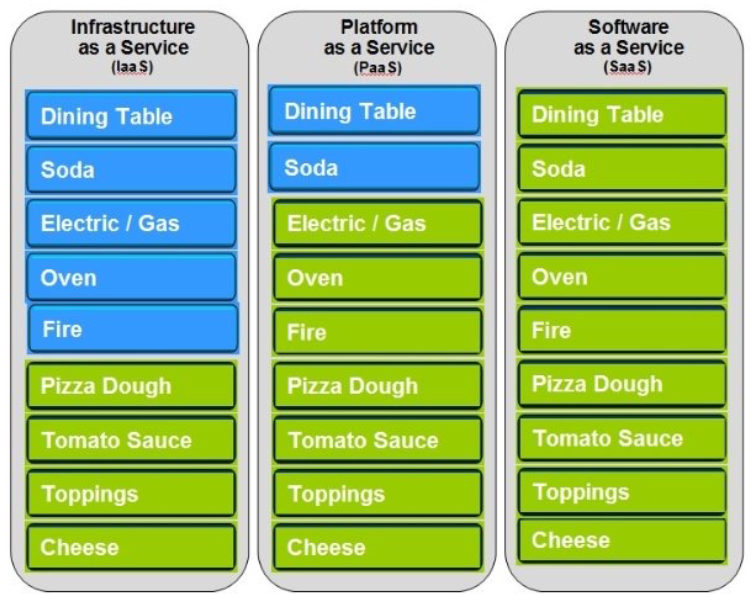
\includegraphics[width=0.8\textwidth]{images/Cloud/PizzaAsAService.png}
    \caption{Pizza as a Service}
    \label{fig:PizzaAsAService}
\end{figure}

\subsection{SaaS}

Before SaaS (\textit{Software as a Service}), software products were initially installed on customers’ computers. Customers had to configure the software and manage software updates, while software product companies had to maintain different product versions. With SaaS, the product is delivered as a service, allowing customers to avoid installation; instead, they pay a subscription and access the product remotely.\\

\noindent
Some benefits of SaaS are:
\begin{itemize}
    \item \textbf{Cash flow}: There is a regular cash flow, which means that customers pay periodic subscriptions or pay-per-use.
    \item \textbf{Update management}: The client controls product updates, so customers receive updates simultaneously. This eliminates the need to maintain multiple versions, resulting in reduced costs.
    \item \textbf{Continuous deployment}: The client can deploy new software versions as soon as changes have been made and tested.
    \item \textbf{Payment flexibility}: Different payment options can attract a wider range of customers (e.g., small companies or individuals can avoid paying large upfront software costs).
    \item \textbf{Try before you buy}: The client can make an early free or low-cost product available to gather customer feedback (e.g., a product free for a few weeks to collect feedback).
    \item \textbf{Data collection}: The client can easily collect data on product usage and customer interactions.
\end{itemize}

\noindent
Some cons of SaaS are:
\begin{itemize}
    \item \textbf{Privacy regulation compliance}: Different countries have varying strict laws regarding the storage of personal information.
    \item \textbf{Security concerns}: Customers may be hesitant to relinquish data control to an external provider, but this data needs to be managed by the SaaS provider. What happens when the SaaS provider experiences a data breach? Will they notify the clients?
    \item \textbf{Network constraints}: These can limit response times during heavy data transfers.
    \item \textbf{Data exchange}: If the cloud does not provide suitable APIs, exchanging data can be difficult. This is contract-based: depending on the offering, you might have access to different sets of data.
    \item \textbf{Loss of control over updates}: This freedom of updates can lead to excessive changes (e.g., new functionalities added daily, impacting the user interface).
    \item \textbf{Service lock-in}: It can be challenging to move code from one SaaS provider to another.
\end{itemize}

\noindent
After deciding that SaaS will be the deployment model, several design issues must be addressed:

\begin{itemize}
    \item \textbf{Local or remote processing}: Some features can be executed locally, which reduces network traffic and increases response speed but may also increase power consumption for battery-powered devices.
    \item \textbf{Authentication}: There are usually three kinds of authentication: the product’s own authentication system, federated authentication (based on mutual trust relationships between a Service Provider (SP) such as an application vendor and an external Identity Provider (IdP)), and individual credentials (e.g., Google, LinkedIn).
    \item \textbf{Information leakage}: If the service is offered to multiple organizations, there's a security risk when a member of one organization handles data belonging to another.
    \item \textbf{Multi-tenant or multi-instance database management}: Multi-tenant systems use a single repository (with advanced techniques to partition data and control those partitions), while multi-instance systems have separate copies of the system and database.
\end{itemize}

\subsection{Multi-tenant and Multi-instance Systems}

\subsubsection{Multi-tenant Systems}
\textit{Multi-tenant systems} use a single database schema shared by all system users. The items in the database are tagged with a tenant identifier to provide “logical isolation,” meaning that users will only be able to access data linked to their tenant, as shown in Figure \ref{fig:multi-tenant-example}.

\begin{figure}[H]
    \centering
    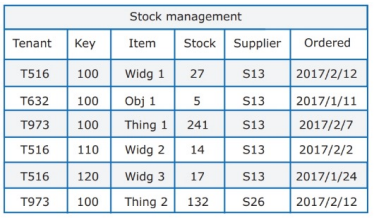
\includegraphics[width=0.6\textwidth]{images/Cloud/multi-tenant-example.PNG}
    \caption{Multi-tenant database schema example}
    \label{fig:multi-tenant-example}
\end{figure}

\noindent
Some advantages of a \textit{multi-tenant system} are:
\begin{itemize}
    \item \textbf{Resource utilization}: The SaaS provider has control over all resources used by the software and can optimize it to make effective use of these resources.
    \item \textbf{Security}: Multi-tenant databases must be designed for security since data for all customers are stored in the same database. They are, therefore, likely to have fewer security vulnerabilities than standard database products. Security management is also simplified as there is only a single copy of the database software to patch if a security vulnerability is discovered.
    \item \textbf{Update management}: It is easier to update a single instance of software rather than multiple instances. Updates are delivered to all customers simultaneously, ensuring that everyone uses the latest version.
\end{itemize}

\noindent
However, there are also challenges associated with a \textit{multi-tenant system}:
\begin{itemize}
    \item \textbf{Inflexibility}: Customers must all use the same database schema, with limited scope for adapting this schema to individual needs.
    \item \textbf{Security}: Since data for all customers is maintained in the same database, there is a theoretical risk of data leaking from one customer to another. More seriously, if there is a database security breach, it can affect all customers.
    \item \textbf{Complexity}: Multi-tenant systems are usually more complex than multi-instance systems due to the need to manage many users, which increases the likelihood of bugs in the database software.
\end{itemize}

Mid-size and large businesses rarely want to use generic multi-tenant software; they often prefer a \textbf{customized version} adapted to their own requirements. One solution is to add extra fields to each table and allow customers to use these fields as they wish. However, predicting how many extra columns to include is challenging (too few will be insufficient, and too many will lead to wasted space), and different customers are likely to need different types of columns. A second solution is to add a field to each table that identifies a separate “extension table,” allowing customers to create these extension tables to reflect their needs. This approach adds a new layer of complexity to a system that is already complex.

\textbf{Security} is the major concern for corporate customers using multi-tenant databases. Since information from all customers is stored in the same database, a software bug or attack could expose the data of some or all customers to others. To mitigate these risks, \emph{multilevel access control} (where access to data is controlled at both the organizational and individual levels) and \emph{encryption of data} (to ensure that corporate users' data cannot be viewed by people from other companies in the event of a system failure) are typically applied. Usually, only sensitive data is encrypted.

\subsubsection{Multi-instance Systems}

A \textit{multi-instance system} allows each customer to have its own system tailored to its needs, including its own database and security controls. This type of system is conceptually simpler than multi-tenant systems and avoids security concerns such as inter-organization data leakage.\\

\noindent
There are two ways to implement multi-instance systems:
\begin{itemize}
    \item \textbf{Virtual Machine-based}: Each software instance and database for a customer runs in its own Virtual Machine. This allows all users from the same customer to access the shared system database.
    \item \textbf{Container-based}: Each user has an isolated version of the software and database running in a set of containers. This solution is best suited for products where users mostly work independently with little data sharing (e.g., for individual users).
\end{itemize}
It is also possible to run containers on a virtual machine: a business could have its own VM-based system and run containers on top of this for individual users.

\newpage
\noindent
Some advantages of a \textit{multi-instance system} are:
\begin{itemize}
    \item \textbf{Flexibility}: Each instance of the system can be tailored and adapted to the customer's needs.
    \item \textbf{Security}: Each customer has its own database, so there's no possibility of data leakage from one customer to another.
    \item \textbf{Scalability}: Instances of the system can be scaled according to the needs of individual customers. For example, some customers may require more powerful servers than others.
    \item \textbf{Resilience}: If a software failure occurs, it will probably affect only a single customer, allowing other customers to continue working as normal.
\end{itemize}

\noindent
However, there are also challenges associated with a \textit{multi-instance system}:
\begin{itemize}
    \item \textbf{Cost}: It is more expensive to use multi-instance systems due to the cost of renting multiple VMs in the cloud and managing multiple systems. Since VMs have a slow startup time, they may need to be rented and kept running continuously, even if there is very little demand for the service. 
    \item \textbf{Update management}: Managing updates for many instances can be complex, especially if the instances have been tailored to specific customer needs.
\end{itemize}

\section{Cloud Software Architecture}

During the initial stages of designing a cloud software architecture, several \textbf{architectural decisions} must be made: Should the software use a multi-tenant or multi-instance database? (\emph{Database organization}) What are the software scalability and resilience requirements? (\emph{Scalability and resilience}) Should the software structure be monolithic or service-oriented? (\emph{Software structure}) The answers to these questions will guide the decision regarding which cloud platform should be used for deployment and delivery.

\subsection{Database Organization}

There are three possible ways to provide a customer database in a cloud-based system:
\begin{enumerate}
    \item As a \textit{multi-tenant system}, shared by all customers of your product. This may be hosted in the cloud using large, powerful servers.
    \item As a \textit{multi-instance system}, with each customer database running on its own virtual machine.
    \item As a \textit{multi-instance system}, with each database running in its own container. The customer database may be distributed across several containers.
\end{enumerate}
\newpage
\noindent
Some factors that can help decide the appropriate method for providing a customer database in a cloud-based system include:
\begin{itemize}
    \item \emph{Target customers}: Do customers require different database schemas and personalization? If so, use a multi-instance database.
    \item \emph{Transaction requirements}: Is it critical that the product supports ACID transactions, ensuring that data is consistently accurate at all times? If so, consider a multi-tenant database or a VM-based multi-instance database.
    \item \emph{Database size and connectivity}: How large is the typical database used by customers? How many relationships exist between database items? A multi-tenant model is usually best for very large databases, as it allows you to focus efforts on optimizing performance.
    \item \emph{Database interoperability}: Will customers wish to transfer information from existing databases? What are the differences in schemas between these and a possible multi-tenant database? What software support will they expect for the data transfer? If customers have many different schemas, a multi-instance database should be used.
    \item \emph{System structure}: Are the developers using a service-oriented architecture for the system? Can the customer database be split into a set of individual service databases? If so, use a containerized multi-instance database.
\end{itemize}

\subsection{Scalability and Resilience}

\subsubsection{Scalability}

Scalability (the ability to adapt automatically to load changes) can be achieved by adding new virtual servers (\textbf{scaling out}) or by increasing the power of an existing server (\textbf{scaling up}) in response to increasing load. Scaling out is typical of cloud-based systems: the product must be organized so that individual software components can be replicated and run in parallel, while load-balancing mechanisms direct requests to different instances of the components (e.g., using PaaS).

\subsubsection{Resilience}

Resilience (the ability to continue delivering critical services in the event of system failure or malicious activity) is realized using a technique known as \textbf{hot standby}, which involves maintaining replicas of software and data in different locations (see Figure \ref{fig:hot-standby}). Database updates are mirrored, and a system monitor continuously checks system status. A cheaper alternative is called \textbf{cool standby}, where, in the event of system failure, the data is restored from a backup (meaning the system will be unavailable until the data restoration is complete).

\begin{figure}[H]
    \centering
    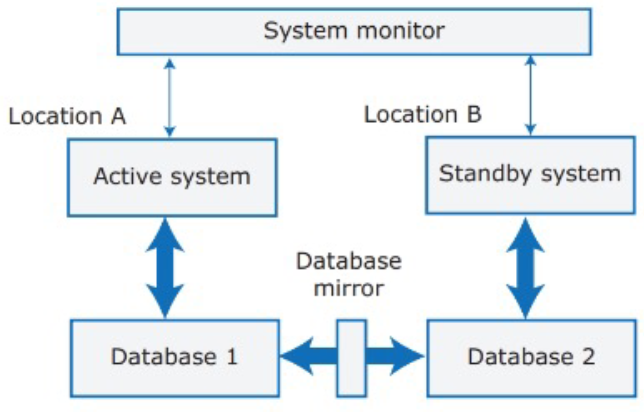
\includegraphics[width=0.6\textwidth]{images/Cloud/hot-standby.png}
    \caption{Hot standby technique schema}
    \label{fig:hot-standby}
\end{figure}

\subsection{Software Structure}

The main choice here is between \textbf{monolithic systems} or \textbf{fine-grained, stateless services}. The latter uses independent services that can be replicated, distributed, and migrated. This approach is particularly suitable for cloud-based software with services deployed in containers. The monolithic approach is often employed to build prototypes, especially if a fine-grained system better fits the specific situation.\\

\noindent
When choosing a cloud platform, there are two main points to consider:

\begin{enumerate}
    \item \textbf{Technical issues}: \emph{Expected load and load predictability}, \emph{resilience}, \emph{supported cloud services} (which cloud services a provider can offer), and \emph{privacy and data protection} (some EU countries have strict requirements regarding data protection and storage locations $\rightarrow$ necessitating cloud providers to offer guarantees on storage locations).
    \item \textbf{Business issues}: \emph{Developer experience} (the languages and technologies depend on the team's experience), \emph{Service-level agreements} (guarantees provided by the cloud provider), \emph{Portability and cloud migration} (to create an ``exit plan'' to mitigate vendor lock-in), \emph{target customers} (customers may have older systems that need to interoperate with the new ones), and \emph{cost} (including all developer and technology-related expenses).
\end{enumerate}

\section{Container Orchestration}

As mentioned in the previous section, containers provide a lightweight mechanism for isolating an application's environment. Container images can be executed reliably on any machine, offering portability (we used Docker) from development to deployment. 

\newpage
\noindent
\textbf{Automated deployment}, such as that provided by Docker, often has limited capability for optimizing memory usage and may not utilize resources effectively. Additional concerns arise: What happens if your container dies? What happens if the machine running your container fails? What if you have multiple containers that need to communicate with one another (\emph{inter-node communication})? How do you enable networking between containers? If your production environment consists of multiple machines, how do you decide which machine to use to run your container?

The solution comes with \textbf{container orchestration}: the architect of a system defines the containers to be run and then hands over control to the \emph{container orchestration platform} to realize that vision.

\subsection{Kubernetes}

One of the most used container orchestration platforms is \textbf{Kubernetes}, which manages the entire lifecycle of individual containers, spinning up and shutting down resources as needed (if a container shuts down unexpectedly, K8s reacts by launching another container in its place). K8s provides a mechanism for applications to communicate with each other even as the underlying individual containers are created and destroyed. Given a set of container workloads to run and a set of machines in a cluster, the container orchestrator examines each container and determines the optimal machine to schedule that workload.

Kubernetes will ingest through its API a ``\emph{Desired State Management},'' which is a YAML manifest. The manifest specifies, given a set of images, which are the \textbf{Pods} (groups of images). Kubernetes will insert inside the same node all the images that are defined in the same Pod, generating as many replicas as defined. A node can handle multiple Pods. If one of the nodes (worker = container host) fails, Kubernetes detects the broken node and starts a new replica, as shown in Figure \ref{fig:K8s5mins}. The \emph{Kubernetes cluster services} not only handle that but also handle communication between the nodes (the existing ones and the ones that will be created).

\begin{figure} [H]
    \centering
    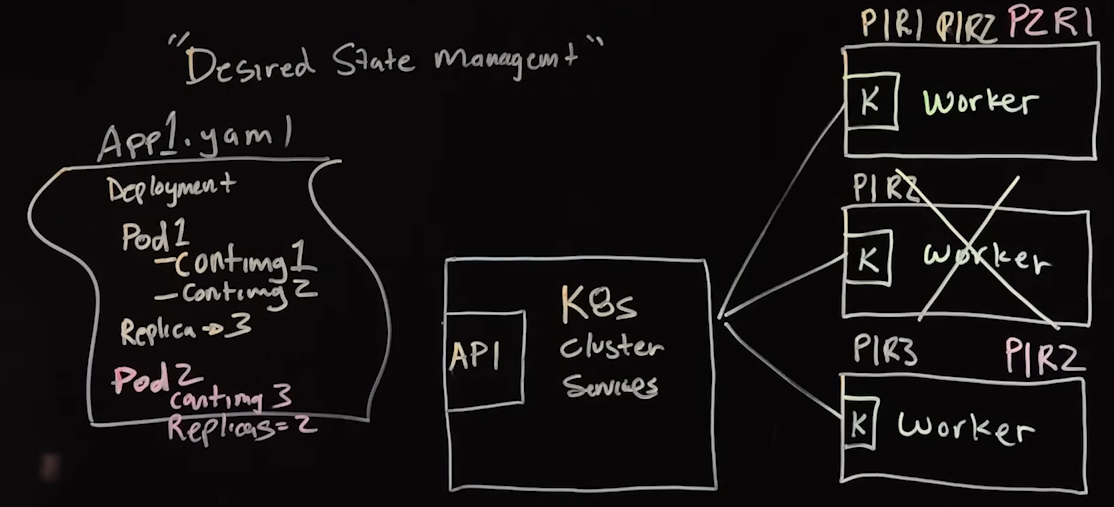
\includegraphics[width=0.8\textwidth]{images/Cloud/K8s5mins.png}
    \caption{Kubernetes' management idea}
    \label{fig:K8s5mins}
\end{figure}

\subsection{Kubernetes Design Principles}

Here are the design principles of Kubernetes:
\begin{itemize}
    \item \textbf{Declarativeness}: A declarative approach is to simply define the desired state of a system (with the manifest). K8s will detect when the actual state of the system doesn't meet our expectations and will intervene to fix the problem, making our system self-healing. The desired state is defined by a collection of objects: each object has a specification in which you provide the desired state and a status that reflects the current state of the object. K8s constantly polls each object to ensure that its status is equal to the specification: if an object is unresponsive, K8s will spin up a new version to replace it; while if an object's status has drifted from the specification, K8s will issue the necessary commands to drive that object back to its desired state.
    \item \textbf{Distribution}: Kubernetes provides a single unified interface for interacting with a cluster of machines. In this way, developers don't have to worry about communicating with each machine individually.
    \begin{figure} [H]
        \centering
        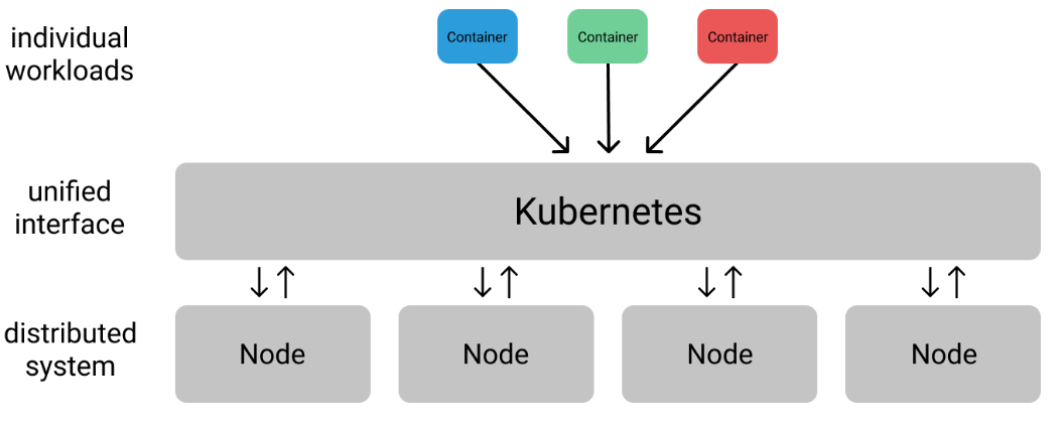
\includegraphics[width=0.75\textwidth]{images/Cloud/K8sDistribution.png}
        \caption{Kubernetes distribution schema}
        \label{fig:K8sDistribution}
    \end{figure}
    \item \textbf{Decoupling}: Containers should be developed with a single concern in mind: microservice-based architecture. K8s naturally supports the idea of decoupled services that can be scaled and updated independently.
    \item \textbf{Immutable infrastructure}: To get the most from containers and container orchestration, an immutable infrastructure should be deployed. This means that instead of logging into a container on a machine to update a library, it is required to build a new container image, deploy the new version, and terminate the older version. The reason is that containers are designed to be ephemeral, ready to be replaced by another container instance at any time. Maintaining immutable infrastructure makes it easier to roll back applications to a previous state (e.g., if an error occurs) by simply updating the configuration to use an older container image.
\end{itemize} 

\subsection{Kubernetes objects}

There are many objects defined by Kubernetes that can be specified in the \textbf{manifests} (either in JSON or YAML). Here's a list of the main ones:
\begin{itemize}
    \item \textbf{Pod}: The minimum Kubernetes deployment unit, which is composed of one or more (tightly related) containers, a shared networking layer, and shared filesystem volumes. Pods can't be distributed by themselves. Each Pod is assigned a unique IP address that we can use to communicate with it.
    \begin{figure} [H]
        \centering
        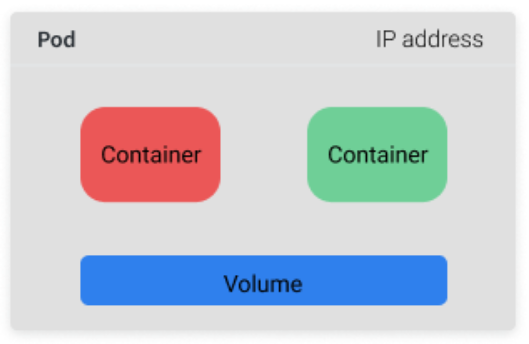
\includegraphics[width=0.6\textwidth]{images/Cloud/K8sPod.png}
        \caption{Kubernetes Pod schema}
        \label{fig:K8sPod}
    \end{figure}
    \item \textbf{Deployment}: It includes a collection of Pods defined by a template and a replica count (number \(n\) of how many copies of the template we want to run). The cluster will always try to have \(n\) Pods available.
    \begin{figure} [H]
        \centering
        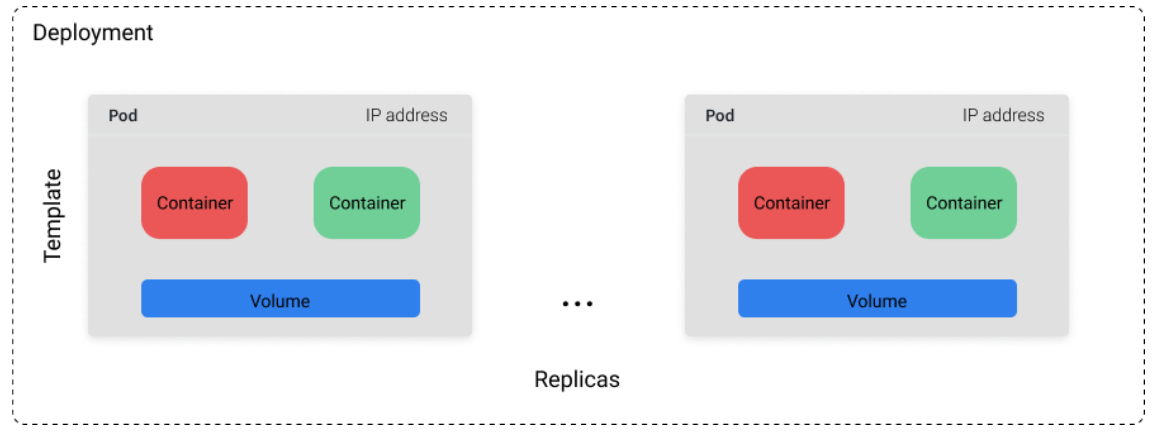
\includegraphics[width=1\textwidth]{images/Cloud/K8sDeployment.png}
        \caption{Kubernetes Deployment schema}
        \label{fig:K8sReplica}
    \end{figure}
    \newpage
    \item \textbf{Service}: The Service object provides a stable endpoint to direct traffic to the desired Pods even as the exact underlying Pods change due to updates/scaling/failures. Services know which Pods they should send traffic to (even if the set of Pods running as part of the Deployment can change at any time) based on labels (key-value pairs) that we define in the Pod metadata.
    \begin{figure} [H]
        \centering
        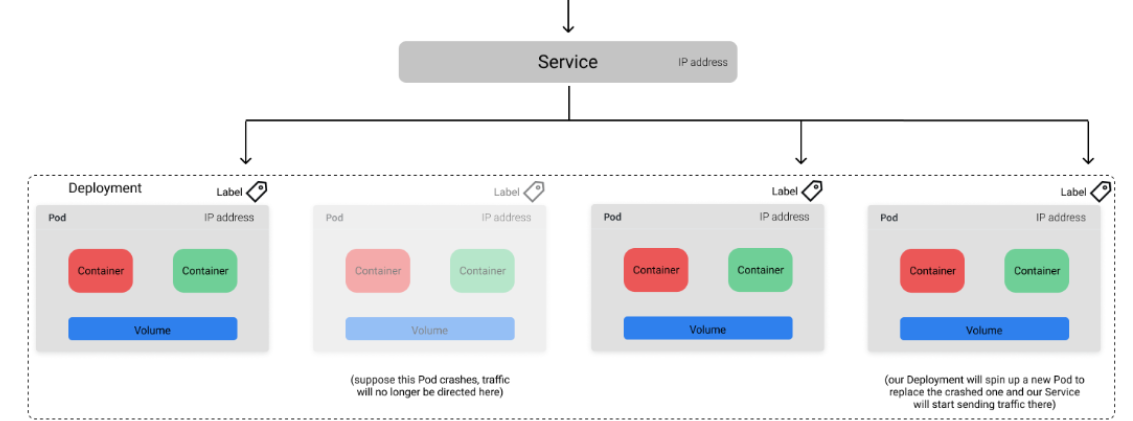
\includegraphics[width=1\textwidth]{images/Cloud/K8sService.png}
        \caption{Kubernetes Service schema}
        \label{fig:K8sService}
    \end{figure}
	\item \textbf{Ingress}: To expose the application to traffic external to the cluster, it is necessary to define an Ingress object. It is possible to select which Services to make publicly available and expose applications behind a stable endpoint (only available to internal cluster traffic).
     \begin{figure} [H]
        \centering
        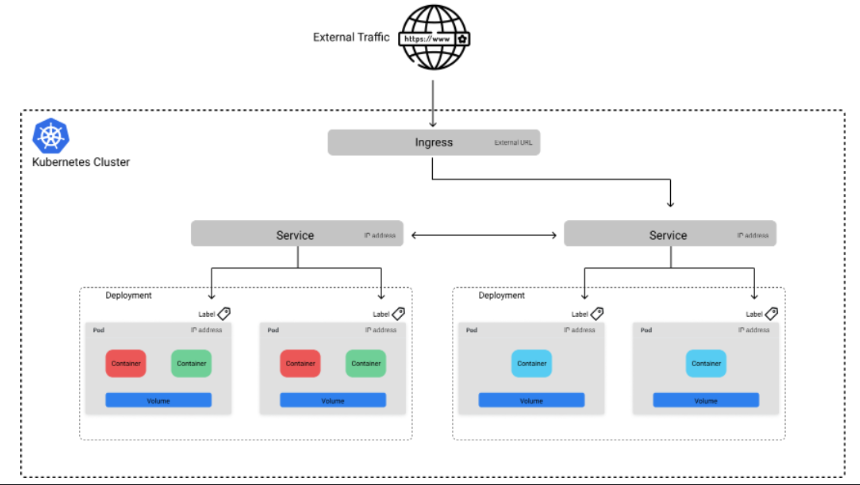
\includegraphics[width=1\textwidth]{images/Cloud/K8sIngress.png}
        \caption{Kubernetes Ingress schema}
        \label{fig:K8sIngress}
    \end{figure}
\end{itemize}

\subsection{Kubernetes control plane}

In this subsection, a high-level description of how Kubernetes works underneath will be provided. There are two types of machines in a cluster (set of machines): the \textbf{master node} (often single), which is a machine that contains most of the control plane components, and the \textbf{worker nodes}, which are machines that run the application workloads.

\subsubsection{Master node}

Users provide new/updated object specifications (manifests) to the API server of the master node. The \textbf{API server} validates update requests (with some input verification) and acts as a unified interface for questions about the cluster's current state. The \emph{state of the cluster} (cluster configuration, object specifications, object statuses, nodes in the cluster, object-node assignments, etc.) is stored in a distributed key-value store named \textit{etcd}.

The Master node (as shown in Figure \ref{fig:K8sMaster}) is composed of the \emph{API Server}, the distributed key-value store \textbf{etcd} (which contains the entire state of the cluster), a \emph{controller-manager}, and a \emph{scheduler}. The reason why the API server works as an intermediary is to reinforce the decoupling principle: each of these components is responsible for only one task (which also makes failure recovery easier).\\

The \textbf{controller-manager} monitors the cluster state through the API server. If the actual state differs from the desired state, the controller-manager will make changes via the API server to drive the cluster towards the desired state.

\begin{figure} [H]
    \centering
    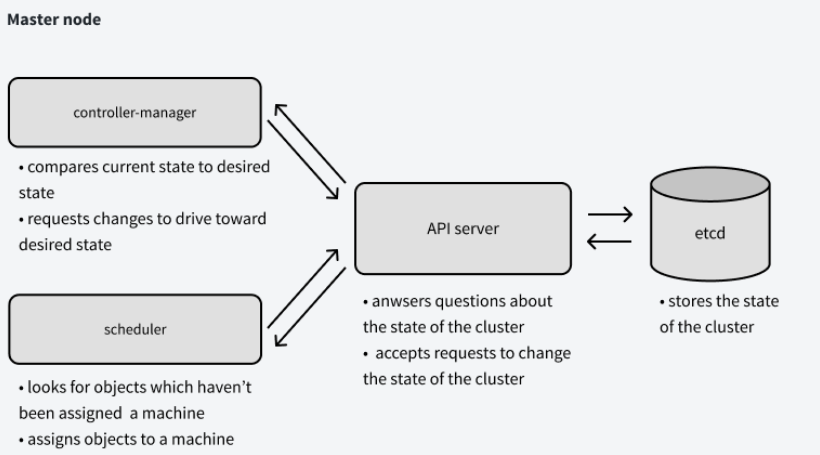
\includegraphics[width=1\textwidth]{images/Cloud/K8sMaster.png}
    \caption{Kubernetes Master node structure}
    \label{fig:K8sMaster}
\end{figure}
\newpage
The \textbf{scheduler} decides where objects should be run, as shown in the below Figure \ref{fig:K8sMasterScheduler}. The scheduler asks the API server which objects haven't been assigned to a machine (1), determines which machines those objects should be assigned to (2), and then replies back to the API server (3) to reflect this assignment (4).

\begin{figure} [H]
    \centering
    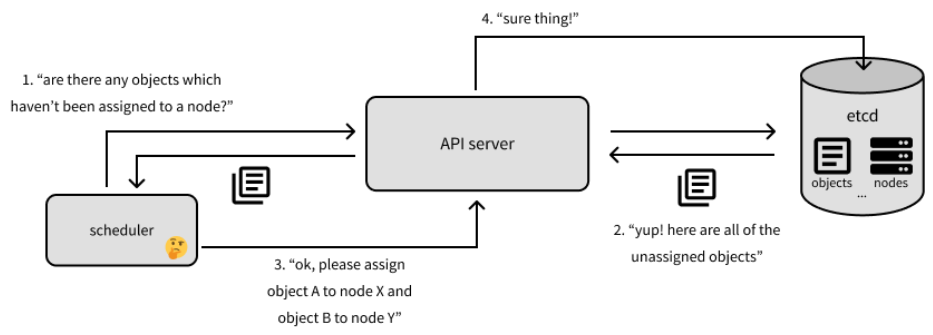
\includegraphics[width=1\textwidth]{images/Cloud/K8sMasterScheduler.png}
    \caption{Scheduler life-cycle}
    \label{fig:K8sMasterScheduler}
\end{figure}

\subsubsection{Worker node}

Every worker node contains a \textbf{kubelet}, which acts as the node's ``agent'' that communicates with the API server to see which container workloads have been assigned to the node. It is responsible for spinning up pods to run these assigned workloads. When a node first joins the cluster, the kubelet announces the node's existence to the API server so the scheduler can assign pods to it.
Workers also contain \textbf{kube-proxy}, which enables containers to communicate with each other across the various nodes in the cluster. With Figure \ref{fig:K8sStructure}, it is possible to observe the entire Kubernetes structure.

\begin{figure} [H]
    \centering
    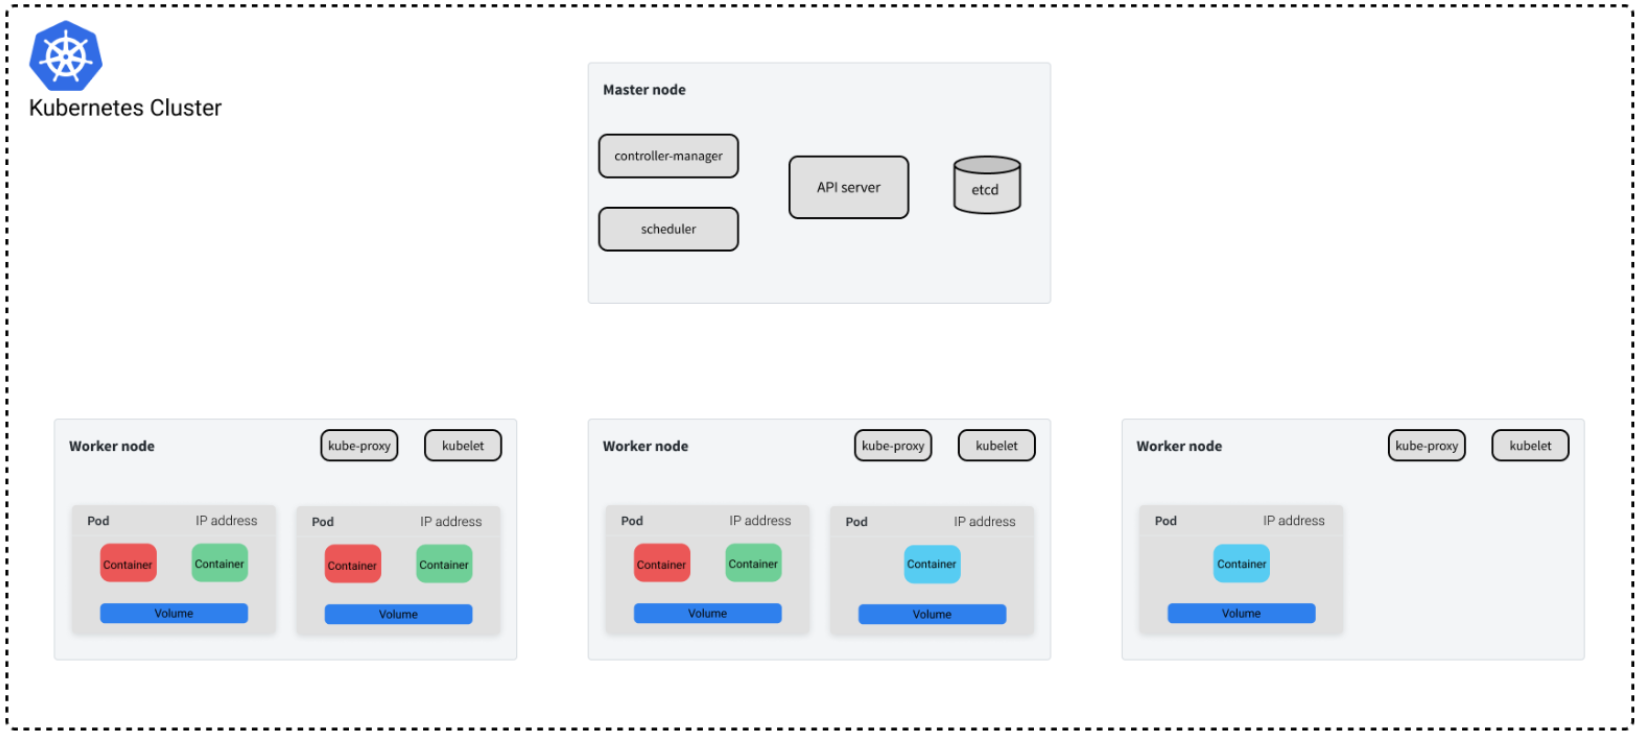
\includegraphics[width=1\textwidth]{images/Cloud/K8sStructure.png}
    \caption{Kubernetes entire structure}
    \label{fig:K8sStructure}
\end{figure}

To conclude this chapter, in which cases is the use of Kubernetes not the best choice?
\begin{itemize}
    \item If you can run your workload on a single machine.
    \item If your compute needs are light.
    \item If you don't need high availability and can tolerate downtime.
    \item If you don't envision making a lot of changes to your deployed services.
    \item If you have a monolith and don't plan to break it into microservices.
\end{itemize}

There's also a way to do container orchestration with Docker (it's called \emph{Docker Swarm}), but Kubernetes is a much stronger orchestrator. Still, they have a partnership, so there's no lock-in between Docker and Kubernetes.


\chapter{Microservices Architecture}

This chapter looks at \textbf{Microservices Architectures}, covering the basic ideas, principles, and benefits that make it popular in modern software development. First, let’s answer an important question: How do we break a system into \textit{components}?

Breaking a system into components is a key step in adopting Microservices Architectures. Here are some reasons for doing this: it allows different teams to work in parallel, promotes reusability, makes it easier to distribute systems across multiple computers, and supports smooth replication, parallel execution, and migration to take full advantage of cloud capabilities like scalability, reliability, and flexibility.

As we explore the main principles of Microservices Architectures, we highlight the importance of stateless services that store \textit{persistent information in local databases}. This approach helps ensure agility and scalability, allowing services to move between virtual servers as needed, while also helping to create resilient and fault-tolerant systems. \\

Software components that can be accessed over the Internet are called \textbf{software services}. A service is accessed through its \textit{published interface}, where all implementation details are hidden. Given an input, a service produces a corresponding output without side effects. Services \textit{do not maintain any internal state} because state information is either stored in an explicit database or maintained by the service requestor. Interactions where the state is maintained involve service requests that have the state and the service result integrated with the answer to the request. \\

\noindent Some history that led to microservices architectures:

\begin{itemize}
    \item \textbf{Service-oriented architecture} (\textbf{SOA}, late 1990s): applications made up of many blocks, where each block is a class or an object. Those (\textit{independent}) blocks could have been written in different technologies since they communicated with each other (or the Internet) through public interfaces.
    \newpage
    \item \textbf{Web Services} (early 2000s): services were standard-based (XML, SOAP, WSDL, and many others), where the standards were used to describe the services (input, output, type of parameters, and so on). Standards were good, but having many standards made them hard to handle.
    \item \textbf{Modern service-oriented systems} (nowadays): much simpler interaction protocols, much simpler interfaces (with more efficient formats for encoding message data), which led to lower overhead and faster execution.
\end{itemize}

Amazon Web Services\footnote{\url{https://aws.amazon.com/}} had a significant impact on this service world, providing a manifesto with guidelines on \textbf{how services should be implemented}: a service should be related to a \textit{single business function}; services should be completely \textit{independent}, with their \textit{own databases}; a service should manage its own user interface; it should be possible to replace/replicate a service without changing other services. This leads to \textbf{microservices}: generally small-scale stateless services that have a single responsibility.

\begin{figure} [H]
    \centering
    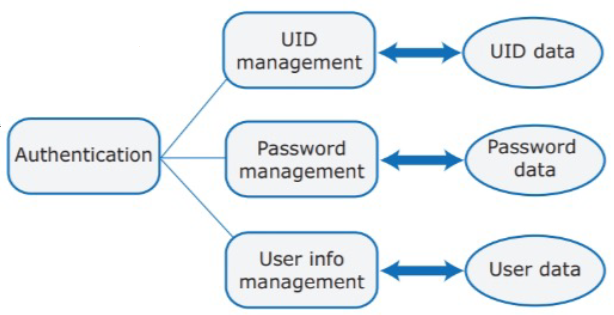
\includegraphics[width=0.7\textwidth]{images/Microservices/service_example.png}
    \caption{Example of a system using an authentication module}
    \label{fig:service_example}
\end{figure} 

Taking a system that uses an authentication module (providing user registration, authentication using UID/password, two-factor authentication, user information management, password reset), we can see from Figure \ref{fig:service_example} an example of a segmentation into microservices. In order to \textit{identify the microservices} that might be used for the authentication system, developers need to break coarse-grained features into more detailed functions, look at the data used, and identify a microservice for each logical data item to be managed (each service will have its own data). In the case that one service needs the data of another service, it can request it through interfaces or just replicate some critical data (facing consistency), minimizing the amount of replicated data management.

\subsection{Microservices}

We have already defined microservices as \textit{independent} (service interfaces not affected by changes to other services) and (generally) small-scale services that can be combined to create applications. It must be possible to modify and redeploy a service without changing/stopping other services.
\newline\noindent
Some of the characteristics that microservices must have are:

\begin{itemize}
    \item \textbf{Self-contained}: Microservices do not have too many external dependencies. They manage their own data and implement their own user interfaces. This allows them to deploy and change the applications immediately.
    \item \textbf{Lightweight}: Microservices communicate using lightweight protocols so that the service communication overhead is low.
    \item \textbf{Implementation independent}: Microservices may be implemented using different programming languages and may use different technologies in their implementation.
    \item \textbf{Implementation deployable}: Each microservice runs in its own process and is independently deployable using automated systems.
    \item \textbf{Business-oriented}: Microservices should implement business capabilities and needs rather than simply provide a technical service. This characteristic coincides with Agile frameworks.
\end{itemize}

Two of the measures used for microservices are \textbf{coupling} (which measures the number of inter-component relationships) and \textbf{cohesion} (which measures the number of intra-component relationships). Developers should achieve \textit{low coupling} and \textit{high cohesion}: \textit{low coupling} means independent services and independent updates, while \textit{high cohesion} means less inter-service communication overhead. \\

Each service should do one thing only, and it should do it well (\textbf{Single Responsibility Principle}). In order to understand \textit{how big a microservice should be}, we can use \textit{the rule of twos}: a service can be developed, tested, and deployed by a team in two weeks. The team can be fed with two large pizzas (8-10 people). 

This amount of people is required because they have to implement service functionality, develop code that makes the service completely independent, process incoming and outgoing messages, manage failures (there will most likely be service and interaction failures), manage data consistency (which becomes severe in the case of data replication) when data are used by other services, maintain the service's own interface, test the service and service interactions, and support the service after deployment (you build it, you run it). Years ago, there were different teams for development and production stages, but now DevOps (the same people who build and maintain the service) is widely used.

\section{Architecture}

The main motivations behind the need for microservices architectures are \textit{shortening lead time for new features and updates} and \textit{scaling}. Deploying microservices in separate containers allows for quickly stopping and restarting the microservice without affecting the other services, and replicas can be quickly deployed. If these two reasons are important for the application, then microservices are the way to go; otherwise (in the case of a simple application), a monolithic application will work just fine.

\begin{figure} [H]
    \centering
    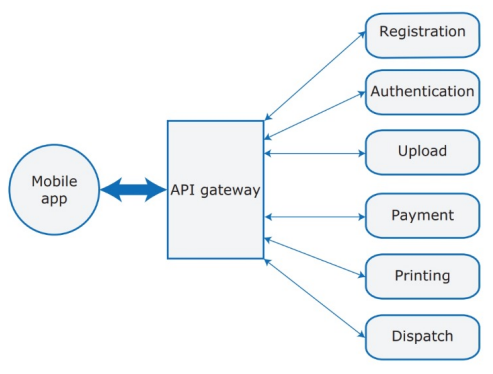
\includegraphics[width=0.65\textwidth]{images/Microservices/photo-printing-system.PNG}
    \caption{Photo-printing system for mobile devices}
    \label{fig:photo-printing-system}
\end{figure} 

From Figure \ref{fig:photo-printing-system}, it's possible to understand that microservices allow us to identify the basic services of an application, as we have separated services for each area of functionality. It also shows that it's good practice to use an \textbf{API gateway} to provide a single point of contact from the mobile application to the microservices. It will be the gateway's job to redirect requests to the appropriate microservice.\\
\newline \noindent
There are five different \textbf{architectural design decisions} that need to be addressed when it comes to microservices architectures:

\begin{enumerate}
    \item What are the microservices that make up the system?
    \item How should microservices communicate with each other?
    \item How should data be distributed and shared?
    \item How should the microservices in the system be coordinated?
    \item How should service failure be detected, reported, and managed?
\end{enumerate}

\noindent These points will be developed throughout the rest of the section.

\subsection{System Decomposition}

The \textbf{system decomposition} is one of the most important design choices, but it is also not an easy task. Having too many microservices will lead to \textit{low cohesion} (which means a lot of communication overhead), while having too few will lead to \textit{high coupling} (which means less independence for updates, deployment, and so on).\\
\newline \noindent Some tips are:
\begin{itemize}
    \item Find the right balance between fine-grained functionality and system performance.
    \item Follow the \textit{common closure principle} (elements likely to be changed at the same time should stay in the same service).
    \item Associate services with business capabilities.
    \item Services should have access only to the data they need (with some data propagation mechanisms).
\end{itemize}

It's usually hard to think in terms of microservices; that's why it's common to start with a monolith and decompose it later. One way to understand how microservices should be split is to look at the data services have to manage.

\subsection{Service Communications}

Another design choice is how the services communicate.

\begin{figure} [H]
    \centering
    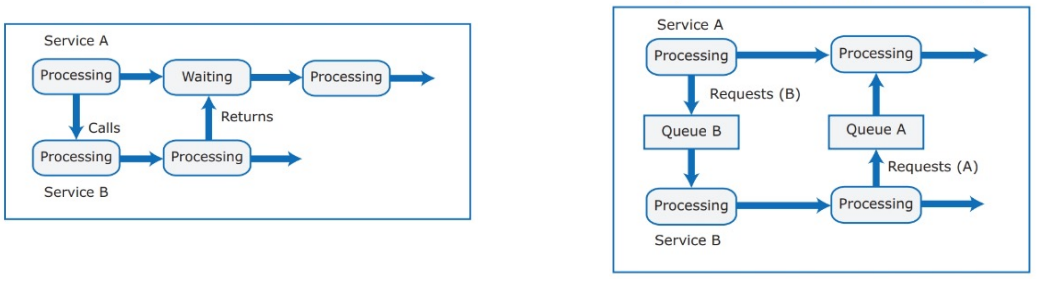
\includegraphics[width=1\textwidth]{images/Microservices/sync-vs-async.PNG}
    \caption{Synchronous vs. asynchronous service interaction}
    \label{fig:sync-vs-async}
\end{figure} 

As shown in Figure \ref{fig:sync-vs-async}, one choice is to go for \textbf{synchronous} or for \textbf{asynchronous} communication: the first one (which in the Figure is the one on the left) is easier to write and understand, while the second one (which in the Figure is the one on the right) has low coupling, is more efficient, but is more difficult to write (since a queue for the requests is required) and to understand.

\begin{figure} [H]
    \centering
    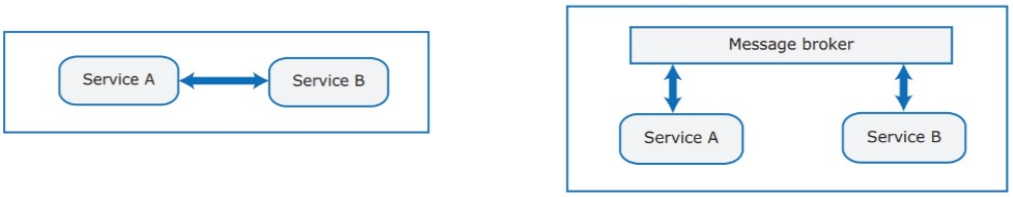
\includegraphics[width=1\textwidth]{images/Microservices/direct-vs-ind.PNG}
    \caption{Direct vs. indirect service communication}
    \label{fig:direct-vs-ind}
\end{figure} 

The second choice is to either choose \textbf{direct} or \textbf{indirect} service communication: the first one consists of allowing one service to send messages directly to another service (it's simpler and faster, but the requester must know the other services' URIs), while the second one utilizes a message broker or a queue that finds the address of the requested service and handles the message translation. The indirect communication supports both synchronous and asynchronous interactions; it is easier to modify and replace services, but it is more complex and slower.

\subsection{Data Distribution and Sharing}

Each microservice should \textbf{manage its own data}, as we want to achieve independence between microservices (so other microservices shouldn't know how data is organized). There will be data dependencies between microservices, and some of the ways to deal with them are:
\begin{itemize}
    \item Data sharing should be as minimal as possible.
    \item Sharing should be read-only, with a few services responsible for data updates.
    \item Include a mechanism to keep database copies used by replicated services consistent.
\end{itemize}

One mechanism to keep database copies consistent is \textbf{ACID}\footnote{ACID: Atomicity, Consistency, Isolation, Durability} \textbf{transactions}, where updates are serialized (which means that the database moves from one consistent state to another) to avoid inconsistency. While in distributed systems we must trade off data consistency and performance, with microservices systems, developers must design the system to \textit{tolerate some degree of data inconsistency}. Two types of data inconsistency that must be managed are:
\begin{itemize}
    \item \textbf{Dependent data inconsistency}: Actions or failures of one service can cause data managed by another service to become inconsistent.
    \item \textbf{Replica inconsistency}: Several replicas of the same service may be executing concurrently, each with its own database copy, and each updating its own database copy (so those databases should be \textit{eventually}\footnote{eventually: sooner or later} \textit{consistent}).
\end{itemize}

\subsubsection{CAP Theorem}

Brewer’s conjecture (PDOC 2000) states that: ``\textit{it is impossible for a web service to provide \textcolor{red}{C}onsistency, \textcolor{red}{A}vailability, and \textcolor{red}{P}artition tolerance at the same time}'', where \textit{\textcolor{red}{C}onsistency} means that each service returns the correct response to each request, \textit{\textcolor{red}{A}vailability} means that each request eventually receives a response, and \newline \textit{\textcolor{red}{P}artition tolerance} means that services can be partitioned into multiple groups, and the network can delay or lose arbitrarily many messages among services. \\

A later reformulation (made in 2012 by Gilbert \& Lynch) states that: \textit{In a network subject to communication failures, it is impossible for any web service to implement an atomic read/write shared memory that guarantees a response to every request} (which implies that you must choose between \textit{consistency} and \textit{availability}). \newline
A simple proof sketch is: Let S1 and S2 be two services belonging to two different network partitions, where every message from S1 to S2 may be delayed or lost. Since S2 can't always be sure whether S1 received the write request or not (because the confirmation from S1 to S2 may be delayed or lost), in the case that S2 sends two different write requests with values V1 and V2, S2 cannot distinguish between the following two cases: S1 received a write request of value V1 and sent an OK response; or S1 received a write request of value V2 and sent an OK response. This leads to a state in S2 that cannot determine whether to return V1 or V2 in response to a read request (because S2 should reply with the same value that S1 does).

\noindent Some practical solutions are:
\begin{itemize}
    \item Guarantee availability and provide best-effort consistency (general solution).
    \item Guarantee strong consistency and provide best-effort availability (this solution is implemented when strong consistency is required (e.g financial applications)).
    \item Trade off consistency and availability (e.g., tolerate being one hour out of date but not one day out of date).
\end{itemize}

\subsubsection{The Saga Pattern}

\begin{wrapfigure}{r}{0.18\textwidth}
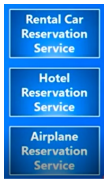
\includegraphics[width=0.18\textwidth]{images/Microservices/Saga.PNG}
    \caption{Saga example}
    \label{fig:Saga}
\end{wrapfigure}

How can we implement distributed transactions with a pattern? \textbf{The Saga pattern} consists of implementing each business transaction that spans multiple services as a \textit{saga}, where a \textit{saga} is a sequence of local transactions (see Figure \ref{fig:Saga}). Each local transaction updates a database and triggers the next local transaction(s) in the saga. If a local transaction fails, then the saga executes a series of compensating transactions (instead of rolling back, since in microservices sometimes rolling back isn't possible).

There are two ways of coordinating sagas: \newline\textbf{Choreography}, where each local transaction publishes events that triggers the next local transaction(s); or \textbf{Orchestration}, where an \newline orchestrator tells participants which local transactions to execute.

There are again two ways of compensating transactions: \newline\textbf{Backward model}, where changes made by previously executed local transactions are undone; and \textbf{Forward model}, where the “retry later” principle is applied. \\

The \textit{Netflix approach} consists of the replication of data in n nodes using \textit{Apache Cassandra}\footnote{\url{https://cassandra.apache.org/_/index.html}} to achieve eventual consistency: the system tries to update as much as possible, ensuring that at least (n/2 + 1) of the replicas must respond. This is one example of a compromise that can be achieved with eventual consistency.

\subsection{Service Coordination}

There are two possible ways to implement \textbf{service coordination}: 
\begin{itemize}
    \item \textbf{Orchestration}, where an orchestrator tells the microservices how they should “play”.
    \item \textbf{Choreography}, where microservices manage themselves.
\end{itemize}
We can think of orchestration as a semaphore and choreography as a roundabout.

\begin{figure} [H]
    \centering
    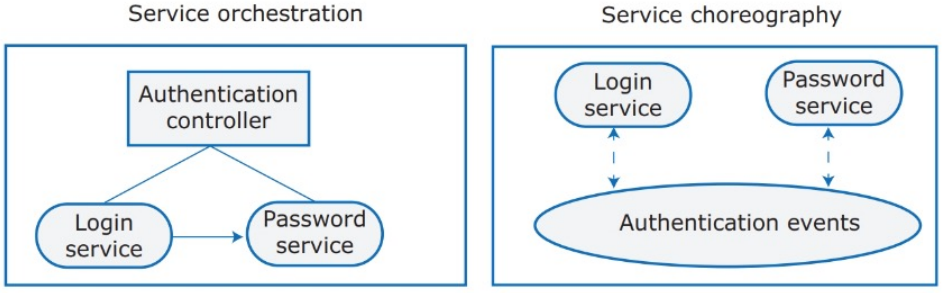
\includegraphics[width=1\textwidth]{images/Microservices/orchestration-vs-choreography.PNG}
    \caption{Example of orchestration and choreography}
    \label{fig:orchestration-vs-choreography}
\end{figure} 

From Figure \ref{fig:orchestration-vs-choreography}, we can see that in the case of service orchestration, there's an explicit controller orchestrating the system (in the example, the controller is named Authentication controller), while in the case of service choreography, an event-based synchronization is used (in the example, a Publish \& Subscribe mechanism named Authentication events). The latter allows for the absence of an additional explicit controller (to avoid single points of failure), but it is harder to debug and recover in case of failure. \\

A good practice is to always start with orchestration (easier to design) and switch to choreography only if the product is inflexible or hard to update.

\newpage

\subsection{Failure management}

Something will go wrong, unavoidably (e.g., a service offers a functionality \(F\) by invoking two other services, each available 99\% of the time and independent of one another. \(F\) will probably be NOT available for around 30 minutes each day). It's important, especially in distributed environments, to have some kind of \textbf{failure management} in case of failure: services must be designed to cope with failures. \\
\newline\noindent
There are mainly three types of failures:
\begin{itemize}
    \item \textbf{Internal service failure}: These are conditions that are detected by the service and can be reported to the service requester in an error message. An example of this type of failure is a service that takes a URL as input and discovers that it is an invalid link.
    \item \textbf{External service failure}: These failures have an external cause that affects the availability of a service. A failure may cause the service to become unresponsive, and actions have to be taken to restart the service.
    \item \textbf{Service performance failure}: The performance of the service degrades to an unacceptable level. This may be due to a heavy load or an internal problem with the service. External service monitoring can be used to detect performance failures and unresponsive services.
\end{itemize}

One of the most typical solutions used for microservices is \textbf{circuit breakers}: they are design patterns that create resilient microservices by limiting the impact of service failures and latencies. The idea is that (take Figure \ref{fig:circuit-breaker} as a reference) an additional component (the circuit breaker) is added between the service client and the remote service (supplier). This additional component takes a request from the client, forwards it to the remote service, and then starts an internal timer. In the case that the remote service works fine, then the additional component receives the answer from the remote service and forwards it to the service client. If the timer triggers a timeout (either because the remote service failed or was too slow), then the circuit breaker tells the client that the remote service failed (avoiding the clients getting stuck waiting for the remote service response). In case of multiple failures, the circuit breaker \textit{trips}, and for the duration of a timeout period, all attempts to invoke the remote service will fail immediately. After the timeout expires, the circuit breaker allows a limited number of test requests to pass through. If those requests succeed, the circuit breaker resumes normal operation. Otherwise, the timeout period begins again.\\

An interesting example of a circuit breaker is implemented by \textit{Spotify}: the search service sometimes fails (since the service has to search through a huge index of songs), so Spotify quickly refreshes the page and uses the time users take to write the name of the song as a cooldown period. Error messages do not pop up.

\begin{figure} [H]
    \centering
    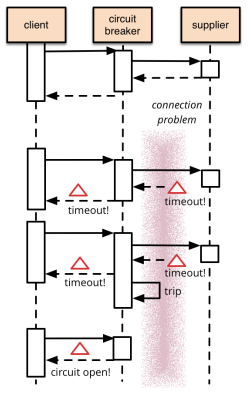
\includegraphics[width=0.4\textwidth]{images/Microservices/circuit-breaker.PNG}
    \caption{Example of a circuit breaker sequence diagram}
    \label{fig:circuit-breaker}
\end{figure} 

There are many ways to test failure management. One interesting way implemented by Netflix is \textit{Chaos Monkey}\footnote{\url{https://netflix.github.io/chaosmonkey/}} (which comes from chaos engineering), a tool that randomly terminates VM instances and containers running inside a production environment. This type of testing is done during the production phase; that's why this is called a \textit{bravely} conducted test.

\section{RESTful services}

Microservices are \textbf{RESTful services}. REpresentational State Transfer (REST) has four main principles:

\begin{itemize}
    \item \textbf{Resource identification through URIs}: the service exposes a set of resources, where each resource is identified by a URI\footnote{Uniform Resource Identifier (URI) is a character sequence that identifies a logical (abstract) or physical resource}.
    \item \textbf{Uniform interface}: clients invoke HTTP methods to create/read/update/delete resources (with POST and PUT to create and update the state of a resource, DELETE to delete a resource, and GET to retrieve the current state of a resource).
    \item \textbf{Self-descriptive messages}: Requests contain enough contextual information to process messages, since information can be accessed in various formats (e.g., HTML, XML, JSON, plain text, PDF, JPEG, etc.). This is why resources are decoupled from their representation.
    \item \textbf{Stateless interactions through hyperlinks}: every interaction with a resource is stateless, which means that servers contain no client state, and any session state is held on the client. Stateless interactions rely on the concept of explicit state transfer.
\end{itemize}

There are many other things to say about REST, but they have already been covered during the bachelor's degree.

\section{Service deployment}

For the past 70 years, for each software project, a group of developers managed the entire life cycle based on project-based software engineering (requirement definition, specifications, prototype, testing, integration, quality of experience, and so on). Once the software is completed, the operations team (which did not participate in the development) puts the software into production (possibly in a different environment from where the software was developed) and then responds to customer problems.

\begin{figure} [H]
    \centering
    \includegraphics[width=0.93\textwidth]{images/Microservices/DevOps.PNG}
    \caption{Continuous Deployment pipeline}
    \label{fig:DevOps}
\end{figure} 

The new era of software engineering is DevOps (a portmanteau of “development” and “operations”): the same team is responsible for service development, deployment, and management. From Figure \ref{fig:DevOps}, we can see the pipeline that software developers use when there's a commit request: the pipeline starts unit tests, makes the build, runs the integration, containerizes, deploys, runs the tests, and if everything goes right, replaces the current service with the new commit.

\subsection{Monitoring}

Testing cannot prevent 100\% of unanticipated problems, which means that there is a need to monitor the deployed services. If you do not monitor microservices, you cannot know the state of the services, but excessive monitoring can lead to performance degradation. As with many things in microservices, a trade-off must be found.

\begin{figure} [H]
    \centering
    \includegraphics[width=0.88\textwidth]{images/Microservices/Monitor-example.PNG}
    \caption{Monitoring example}
    \label{fig:Monitor-example}
\end{figure} 

The example shown in Figure \ref{fig:Monitor-example} illustrates that it's also possible to increase reliability with monitoring: when a new version of a service is introduced, it's possible to maintain the old version while changing the “current version link” to point to the new service. If monitoring detects a problem with the new version of the “Cameras 002” service, it switches the “current version link” back to version 001 of the Cameras service.


\section{Architectural smells}

An \textbf{architectural smell} is a commonly used architectural decision that negatively impacts system lifecycle qualities. Once the microservice principles are defined, how can architectural \textcolor{red}{smells} affecting the design \textcolor{blue}{principles} of microservices be detected and then resolved via \textcolor{green}{refactoring}?

This section will show, based on a \textit{multivocal review} (which uses both scientific articles and technical websites), the most recognized \textit{architectural smells} for microservices and the architectural \textit{refactorings} to resolve them. \newline The \textbf{design principles} that will be taken into consideration are:

\begin{itemize}
    \item \textcolor{blue}{Independent deployability}: the microservices forming an application should be independently deployable.
    \item \textcolor{blue}{Horizontal scalability}: the microservices forming an application should be horizontally scalable (which means the possibility of adding/removing replicas of individual microservices).
    \item \textcolor{blue}{Isolation of failures}: failures should be isolated (avoiding the cascade effect).
    \item \textcolor{blue}{Decentralization}: decentralization should occur in all aspects of microservice-based applications, from data management to governance.
\end{itemize}

\subsection{Smells and refactoring}

All the \textcolor{red}{architectural smells} will be categorized based on the \textcolor{blue}{design principle} they violate. For each smell, some \textcolor{green}{refactorings} will be presented to resolve them.

\subsubsection{Independent deployability}

One \textit{architectural smell} for \textcolor{blue}{independent deployability} is \textcolor{red}{multiple services in one container} (because ideally we want to have one container per microservice). It is possible to insert some microservices that interact a lot inside the same container, but this can lead to various problems. The solution for this smell is to \textcolor{green}{package each service in a separate container}.

\subsubsection{Horizontal scalability}

One common \textit{architectural smell} for \textcolor{blue}{horizontal scalability} is \textcolor{red}{endpoint-based service interaction}. This is a smell because, if there is an interaction with a specific service instance (as shown in Figure \ref{fig:end-point-img1}), adding more replicas of the service won't scale the application since the interaction is made with only one of the replicas. Some \textit{refactorings} for the described \textit{smell} are to \textcolor{green}{add a service discovery} that will indicate to the requester which replica they must use (applied in 55\% of cases), \textcolor{green}{add a message router} that will redirect the request to one of the replicas (e.g., load balancer, applied in 31\% of cases), or \textcolor{green}{add a message broker} that will collect the requests, which are then processed by the replicas (e.g., message queue, applied in 14\% of cases). The reason that the message broker is the least used is that the code of the microservice has to be modified.

\begin{figure} [H]
    \centering
    \includegraphics[width=0.65\textwidth]{images/Microservices/end-point-img1.PNG}
    \caption{Endpoint-based service interaction}
    \label{fig:end-point-img1}
\end{figure} 

Another \textit{architectural smell} is the \textcolor{red}{absence of an API gateway}, because clients can invoke the services directly (which is similar to the endpoint-based service interaction smell). The solution is simply to \textcolor{green}{add an API gateway}, as it not only resolves the smell but can also be useful for authentication, throttling, and so on.

\newpage 

\subsubsection{Isolation of failures}

One \textit{architectural smell} for \textcolor{blue}{isolation of failures} is \textcolor{red}{wobbly service interaction}: the interaction of m1 with m2 is \textit{wobbly} when a failure of m2 can trigger a failure of m1. Some \textit{refactorings} for the described \textit{smell} are to \textcolor{green}{add a circuit breaker} (applied in 42\% of cases), \textcolor{green}{use timeouts} (applied in 22\% of cases), \textcolor{green}{add a bulkhead} (applied in 20\% of cases), or \textcolor{green}{add a message broker} (applied in 16\% of cases).

\subsubsection{Decentralization}

One common \textit{architectural smell} for \textcolor{blue}{decentralization} is \textcolor{red}{shared persistence}. Three proposed solutions (which are better described in Figure \ref{fig:shared_persistence}) are \textcolor{green}{split database} (applied in 50\% of cases), \textcolor{green}{add a data manager} that acts as a gateway between the services and the database (applied in 22\% of cases), or \textcolor{green}{merge services} (applied in 9\% of cases).

\begin{figure} [H]
    \centering
    \includegraphics[width=1\textwidth]{images/Microservices/shared_persistence.PNG}
    \caption{Solutions for shared persistence}
    \label{fig:shared_persistence}
\end{figure} 

The last \textit{architectural smell} is the \textcolor{red}{single-layer teams}, which goes against the idea of Agile. The solution is simply to \textcolor{green}{split teams by service}.

\subsection{A toolchain for microservices}

Now that we know about these \textit{architectural smells}, we want to identify and solve them. The first step is to create a graphical representation of our architecture, as shown in Figure \ref{fig:modelling-application-architecture}. This is done to better understand the structure of the application.

These models also allow for \textit{team-based views}, as each service is developed by a different team. This is particularly useful in cases where there may be smells between two or more microservices managed by different teams. It enables teams to detect these smells and make necessary arrangements to address and fix them.

\begin{figure} [H]
    \centering
    \includegraphics[width=1\textwidth]{images/Microservices/modelling-application-architecture.PNG}
    \caption{Modelling application architecture}
    \label{fig:modelling-application-architecture}
\end{figure} 

There are tools that take these models as input and provide, as output, the smells present in the application. One developed by the University of Pisa is MicroFreshner\footnote{\url{https://github.com/di-unipi-socc/microFreshener}}. It may be hard to obtain the modeled application architecture in the case of a large system, so tools have been created (such as MicroMiner and MicroTOM) to obtain those models by providing the K8s manifest and performing some dynamic analysis of the running application (noting that container orchestration does change application behavior). From Figure \ref{fig:toolchain}, we can see the toolchain used to fix microservices smells.

\begin{figure} [H]
    \centering
    \includegraphics[width=1\textwidth]{images/Microservices/toolchain.PNG}
    \caption{Toolchain for microservices}
    \label{fig:toolchain}
\end{figure} 

Once the smells have been analyzed and some fixes have been made inside MicroFreshner, it is possible to take the result of MicroFreshner and automatically deploy the fixed architecture on top of the existing container orchestrator.



\chapter{Security and Privacy}

Software security is a high-priority concern for both product developers and users (since malicious attacks can cause losses to both). Figure \ref{fig:threats-security} shows the main types of security threats, even though there are some attacks that combine those threats (e.g., a ransomware attack threatening the integrity of system data also threatens system availability).

\begin{figure} [H]
    \centering
    \includegraphics[width=0.8\textwidth]{images/Security/threats-security.png}
    \caption{Main types of security threats}
    \label{fig:threats-security}
\end{figure} 

Security is a \textbf{system-wide issue}: application software depends on the operating system, web server, language run-time system, database, frameworks, tools, and so on. Attacks may target any level of the system infrastructure stack, starting from the network.

\newpage
\noindent Some system management activities to maintain security are:
\begin{itemize}
    \item \textbf{Authentication and authorization standards and procedures} to ensure that all users have strong authentication and properly set up access permissions.
    \item \textbf{System infrastructure management} to keep infrastructure software properly configured and to promptly apply security updates patching vulnerabilities.
    \item Regularly \textbf{monitoring attacks} to promptly detect them and trigger resistance strategies to minimize the effects of an attack.
    \item \textbf{Backup policies} to keep undamaged copies of program and data files that can be restored after an attack.
\end{itemize}

\section{Attacks and defenses}

\subsection{Injection attacks}

An injection attack happens when a malicious user uses a valid input field to input malicious code or database commands to damage the system. One of the most common classes of attacks is \textbf{buffer overflow attacks}, which occur when an attacker can carefully craft an input string that includes executable instructions and overwrites memory. If a function return address is overwritten, control can be transferred to malicious code (e.g., on operating systems/libraries written in C/C++, which do not check whether array assignments are within array bounds).

Another common class of attacks is \textbf{SQL injection attacks}, which occur when an attacker can do an injection attack when user input is part of an SQL command. An easy countermeasure is to check input validity.

\subsection{Session hijacking attacks}

In many applications, there's the concept of a \textit{session}, which is a time period during which a user’s authentication with a web app is valid. This is usually achieved with session cookies (tokens) sent from the server to the client in each HTTP request, so the user doesn’t have to re-authenticate for subsequent system interactions (the session is closed when the user logs out or when the system “times out”).

Session hijacking is performed by an attacker who wants to acquire a valid session cookie in order to \textbf{impersonate a legitimate user}. An attacker can obtain the session cookie with a cross-site scripting attack or with traffic monitoring (which is easy on unsecured Wi-Fi networks and unencrypted data). The attack can either be \textbf{active} (the attacker carries out user actions on a server) or \textbf{passive} (the attacker simply monitors client-server traffic looking for valuable information, such as passwords, credit card numbers, and so on).

Some trivial defenses for this type of attack are to \textit{encrypt client-server network traffic} (using, for example, HTTPS), use \textit{multifactor authentication} to require confirmation of new actions that may be damaging, and use relatively \textit{short timeouts} on sessions.

\subsection{Cross-site scripting attacks}

Another form of injection attack is cross-site scripting attacks, where the attacker \textbf{adds malicious JavaScript code to the web page} returned from server to client. The malicious script is executed when the page is displayed in the victim’s browser, with the intention of stealing customer information or directing customers to another website (cookies may be stolen, making a session hijacking attack possible).

\begin{figure} [H]
    \centering
    \includegraphics[width=0.93\textwidth]{images/Security/XSS.png}
    \caption{Cross-site scripting attack}
    \label{fig:XSS}
\end{figure} 

Some defenses for this kind of injection are (form) input validation, checking input from the database before adding it to the generated page, and employing the HTML “encode” command (info added to the web page is not executable).

\subsection{Denial-of-Service attacks}

Denial-of-Service attacks (DoS attacks) are intended to \textbf{make system unavailable} for normal use. This is usually performed with the usage of distributed computers (that have usually been hijacked) that are sending hundreds of thousands of requests for service to a web application. Those attacks aims to boycott server provider or to demand ransom payment. For this attack there are specialised software for detecting and dropping incoming packets, which helps to prevent the flooding of requests. More contermeasures are temporary user lockouts (e.g. lockout user by repeatedly failing authentication with user email address as login name), and IP address tracking (to restrict lockout when failed logins come from unusual IP addresses).

\subsection{Brute force attacks}

An attacker has only some information (e.g., a valid login name, but not the password) and repeatedly tries to guess the missing information. An attacker can use a string generator to \textbf{generate all possible combinations} of letters and numbers. The defenses for this type of attack are to convince (which means force) users to set long passwords that are not in a dictionary and are not common words. Another security layer can be added with the use of two-factor authentication.

\section{Authentication and Authorization}

\subsection{Authentication}

The objective of authentication is ensuring that users of your system are who they claim to be. Some approaches to achieve authentication are:
\begin{itemize}
    \item \textbf{Knowledge-based authentication} relies on users providing secret, personal information when registering. This type of authentication has weaknesses, such as \textit{insecure passwords}, \textit{phishing attacks} (users click on an email link pointing to a fake site that collects login and password), users using the \textit{same password}, and users regularly \textit{forgetting passwords} (a password recovery mechanism is needed, which means potential vulnerability if credentials have been stolen). Some ways to make this authentication method more secure are to force users to set strong passwords and to add personal questions for password recovery.

    \item \textbf{Possession-based authentication} relies on users having a physical device that can be linked to the authenticating system and that generates/displays information known to the authenticating system (e.g., the system sends a code to the user’s phone number or a special-purpose device that generates one-time codes).
    
    \item \textbf{Attribute-based authentication} relies on a unique biometric attribute of the user (e.g., fingerprint, face).
\end{itemize}

In cases where a system wants to store confidential user information, multi-factor authentication (e.g., password, then a code received on a mobile phone) is the best practice in order to add another layer of security.

Usually, developers don't implement authentication from scratch, but they use available toolkits and libraries (e.g., OAuth\footnote{\url{https://oauth.net/2/}}). Even when using already implemented libraries, there is still a lot of programming effort involved in order to implement a secure and reliable authentication system. This is why authentication systems are often outsourced with a \textbf{federated identity system}, which means using an external service for authentication (e.g., Google, Facebook, and so on), as shown in Figure \ref{fig:federated-identity}. These external services for authentication are proven to be secure and are likely to be much better than any independent system implemented by the product provider. On top of that, it allows the product provider to avoid maintaining their own database of passwords/secrets, as well as to gain additional user information (if the user agrees).

\begin{figure} [H]
    \centering
    \includegraphics[width=0.85\textwidth]{images/Security/federated-identity.png}
    \caption{Federated identity sequence diagram}
    \label{fig:federated-identity}
\end{figure} 

\textbf{Mobile device authentication} plays by different rules, since usually typing passwords on mobile keyboards is inconvenient. An alternative to the written password could be to install an \textit{authentication token} on the mobile device, but this would lead to some weaknesses (if the device is stolen/lost, someone else can get access to the product). A safer alternative is to use \textit{individual users' digital certificates} (issued by trusted providers).

\subsection{Authorization}

While \textit{authentication} aims to ensure that the user is who they claim to be, \textit{authorization} wants to control that the user can access resources. It is required to have \textbf{access control} for multiuser products, where the access control policy \textit{must} reflect data protection rules that limit access to personal data (to prevent legal actions in case of a data breach).

One popular way to implement an access control policy is with \textbf{Access Control Lists} (ACLs): users are classified into groups (which dramatically reduces the size of ACLs), different groups can have different rights on different resources, and hierarchies of groups allow assigning rights to subgroups/individuals. We can see an example of an Access Control List in Figure \ref{fig:ACLs}.

\begin{figure} [H]
    \centering
    \includegraphics[width=0.85\textwidth]{images/Security/ACL.png}
    \caption{Example of Access Control Lists}
    \label{fig:ACLs}
\end{figure}

\section{Encryption}

\textit{Encryption} consists of making a text (typical data) unreadable by applying an algorithmic transformation to it. The text is encrypted with a secret key, travels through unsafe channels, and is then encrypted with the same or another key when it reaches its destination.

\textit{Modern encryption} techniques are considered “practically uncrackable” using currently available technology, even if history tells us that apparently uncrackable encryption may become crackable when new technology becomes available (what if/when quantum computers become commercially available one day?).

\noindent Usually, encryption is divided into two categories:

\begin{itemize}
    \item \textbf{Symmetric encryption}: older than the other method, used for centuries, but still used nowadays. Symmetric encryption uses the same key for encoding and decoding, but the sharing of the key is the weakness of this type of encryption.
    \item \textbf{Asymmetric encryption}: Asymmetric encryption uses different keys for encoding and decoding. This is the most secure encryption method, but also the most expensive one in terms of computation required for key generation. It's common practice to start the communication between two subjects using asymmetric encryption to share a symmetric key for the rest of the communication. 
\end{itemize}

\noindent\textbf{Transport Layer Security} (TLS) is a widely adopted security protocol designed to facilitate privacy and data security for communications over the Internet. A primary use case of TLS is encrypting the communication between web applications and servers, such as web browsers loading a website. This protocol can be built on top of the HTTP protocol, generating \textbf{HTTPS}, which is a standard practice for websites. TLS is also used to verify the identity of web servers with the use of \textbf{digital certificates} sent from servers to clients. Digital certificates are issued by trusted identity verification services (CAs). An example of a typical client-server handshake is shown in Figure \ref{fig:TLS}.

\begin{figure} [H]
    \centering
    \includegraphics[width=0.8\textwidth]{images/Security/TLS.png}
    \caption{TLS client-server interaction to generate symmetric key for exchanging data}
    \label{fig:TLS}
\end{figure} 

\noindent It's interesting to understand when user data should be encrypted, and to do so we'll categorize data into:
\begin{itemize}
	\item \textbf{Data in transit} should always be encrypted since we want to achieve privacy in our communications.
	\item \textbf{Data at rest} (stored) should always be encrypted: in case of attacks, we don't want the attackers to obtain users' information in clear text.
	\item Encrypting and decrypting \textbf{data in use} (i.e., actively processed) slows down system response time.
\end{itemize}

\noindent Encryption of data is possible at four different levels in the system:
\begin{itemize}
	\item \textbf{Application level}: The application decides what data should be encrypted and decrypts that data immediately before it is used. This not only causes performance issues (security doesn't come for free), but it also requires some sort of key management. 
	\item \textbf{Database level}: The DBMS may encrypt the entire database when it's closed, with the database decrypted when it is reopened. Alternatively, individual tables or columns may be encrypted or decrypted.
	\item \textbf{Files level}: The operating system encrypts individual files when they are closed and decrypts them when they are reopened.
	\item \textbf{Media level}: The operating system encrypts disks when they are unmounted and decrypts these disks when they are remounted (useful for stolen/lost laptops).
\end{itemize}

All those levels require a key in order to encrypt and decrypt data. Data protection regulations may require that data copies are kept for years and stored securely, which means that if encryption keys get lost, encrypted data become permanently inaccessible! Keys should be changed periodically, and the database must maintain multiple timestamped versions of keys. To make life easier, \textbf{Key Management Systems} (KMS) are used to ensure that keys are securely generated, stored, and accessed by authorized users. Figure \ref{fig:KMS} shows how KMS are used.

\begin{figure} [H]
    \centering
    \includegraphics[width=0.7\textwidth]{images/Security/KMS.png}
    \caption{KMS usage schema}
    \label{fig:KMS}
\end{figure} 

\section{Privacy}

Privacy is a social concept that relates to the collection, dissemination, and appropriate use of personal information held by a third party.

\begin{figure} [H]
    \centering
    \includegraphics[width=0.9\textwidth]{images/Security/privacy-laws.png}
    \caption{Data protection laws}
    \label{fig:privacy-laws}
\end{figure} 

\noindent Some data protection principles are:
\begin{itemize}
    \item \textbf{Awareness and Control}: Users of your product must be made aware of what data is collected when they are using your product and must have control over the personal information that you collect from them.
    \item \textbf{Purpose}: You must tell users why data is being collected, and you must not use that data for other purposes.
    \item \textbf{Consent}: You must always have the consent of a user before you disclose their data to other people.
    \item \textbf{Data lifetime}: You must not keep data for longer than you need to. If a user deletes an account, you must delete the personal data associated with that account.
    \item \textbf{Secure storage}: You must maintain data securely so that it cannot be tampered with or disclosed to unauthorized people.
    \item \textbf{Discovery and error correction}: You must allow users to find out what personal data you store. You must provide a way for users to correct errors in their personal data.
    \item \textbf{Location}: You must not store data in countries where weaker data protection laws apply unless there is an explicit agreement that some stronger data protection rules will be upheld. 
\end{itemize}

\noindent There are also \textit{business reasons} for paying attention to information privacy:

\begin{itemize}
	\item If the system's conformance to privacy regulations does not match data protection regulations, the provider may be subject to legal actions or may not be able to sell their product.
	\item If a provider sells a business product, the provider's business customers may require privacy safeguards (not to be at risk with their users).
	\item Leakage or misuse of client information can damage the provider's reputation.
\end{itemize}

\noindent The information that software needs to collect depends on the functionality of the product and on the business model the provider uses. Here are more tips about data privacy:

\begin{itemize}
	\item Do not collect personal information that you do not need.
    \item Establish a privacy policy defining how personal/sensitive information about users is collected, stored, and managed.
	\item Make clear if you use users’ data to target advertising or to provide services that are paid for by other companies.
	\item If your product includes social network functionalities so that users can share information, you should ensure that users understand how to control the information they share.
\end{itemize}

\section{Security Smells}

\subsection{Challenges of Securing Microservices}

This subsection will outline the general properties of attacks and security specific to microservices. The illustration will be made with a list of key points:

\begin{itemize}
    \item \textit{The broader the attack surface, the higher the risk}: Since microservices trade data between each other using inter-service communication via remote calls, this means that (potentially) there are a large number of entry points, which \textbf{broadens the attack surface}. The security of the application depends on the weakest link: only one weak entry point can compromise the whole application.
    \item \textit{Distributed security screening affects performance}: Each microservice has to carry out independent security screening. This means that each service may need to connect to a remote security token service. Repeated, distributed security checks affect \textbf{performance}. A workaround for this problem is to \textit{trust the network} and skip security checks at each microservice, but a real solution (and also an industry trend) is to use \textit{zero-trust networking principles}, though overall performance must be considered.
    \newpage
    \item \textit{Bootstrapping trust among microservices needs automation}: Service-to-service communication must take place on protected channels. Suppose those services are using \textit{certificates}; each microservice must be provisioned with a certificate (and corresponding private key) to authenticate itself to another microservice during service-to-service interactions. The receiver must know how to validate the certificate of the calling microservice, so there is a need to \textbf{bootstrap trust} between microservices (including the need to revoke and rotate certificates). To manage large-scale deployments of hundreds of microservices, \textit{automation} is needed.
    \item \textit{Tracing requests spanning multiple microservices is challenging}: Logs can be aggregated to produce \textit{metrics} that reflect system state (e.g., average invalid access requests per hour) and may trigger alerts. Traces help track a request from the point where it enters the system to the point where it leaves. Unlike monolithic applications, a request in a microservices deployment may span multiple microservices, making \textbf{correlating requests among microservices challenging}.
    \item \textit{Containers complicate credentials/policies handling}: Containers are \textit{immutable servers} (great for simplifying deployment and achieving horizontal scalability), so they don’t change state after spin-up. Since each service needs to maintain a dynamic list of allowed clients and a dynamic set of access-control policies, the only way to modify these lists periodically is to keep credentials in the container filesystem and \textbf{inject them at boot time}.
    \item \textit{Distribution makes sharing user context harder}: When a request starts to move inside the system, there is a lot of information we want to associate with the request (e.g., whether it’s a premium or non-premium request). The challenge is to \textit{build trust between microservices} so that the receiving microservice accepts the user context passed from the calling microservice (a security attack can occur if user information is manipulated). A popular solution is \textbf{JSON Web Token} (JWT), a security token used to share user context among microservices.
    \item \textit{Security responsibilities distributed among different teams}: Different independent teams can use \textbf{different technology stacks} (such as security best practices and various tools for static and dynamic security testing). Security responsibilities are distributed across different teams. Organizations often adopt a hybrid approach with a centralized security team and security experts within the teams.
\end{itemize}
\newpage
\subsection{Smells and Refactoring}

A \textbf{security smell} is a commonly used architectural decision that indicates possible security violations in microservice-based applications. Once the microservice principles are defined, how can \textcolor{red}{security smells} that affect \textcolor{blue}{security properties} of microservices be detected and resolved via \textcolor{green}{refactoring}?

This section will show, based on a \textit{multivocal review} (which uses both scientific articles and technical websites), which are the most recognized \textit{security smells} for microservices and the security \textit{refactorings} to resolve them. 

\noindent The \textbf{security properties} that will be considered are:

\begin{itemize}
    \item \textcolor{blue}{Confidentiality}: The degree to which a product or system ensures that data is accessible only to those authorized to have access.
    \item \textcolor{blue}{Integrity}: The degree to which a system, product, or component prevents unauthorized modification of computer programs or data.
    \item \textcolor{blue}{Authenticity}: The degree to which the identity of a subject or resource can be proven to be the one claimed.
\end{itemize}

\noindent Since some \textit{security smells} violate multiple \textit{security properties}, the following list will show all the \textcolor{red}{security smells}, their related \textcolor{blue}{security properties}, and how to \textcolor{green}{refactor} them:

\begin{itemize}
    \item \textcolor{red}{Insufficient access control}: Some services of an application don't implement access control, leading to a \textit{confused deputy problem} (an attacker obtaining data they shouldn’t access), causing potential violations of the \textcolor{blue}{confidentiality} of data (and business functions). Client permissions need to be verified at request time without introducing extra latency and contention with frequent calls to a centralized service. One way to refactor this smell is to \textcolor{green}{use OAuth 2.0}, a token-based security framework for delegated access control.
    \item \textcolor{red}{Publicly accessible microservices}: Some microservices are directly accessible by external clients. Each such microservice must check authentication and authorization for each request (increasing the cost of application maintenance), but this also increases the exposure of credentials, which could lead to \textcolor{blue}{confidentiality} violations. The most cited refactoring is the \textcolor{green}{implementation of an API gateway}, which can (from behind a firewall) enforce authentication, authorization, throttling, and message content validation.
    \item \textcolor{red}{Unnecessary privileges to microservices}: Sometimes microservices are granted unnecessary access levels, permissions, or functionalities that are not needed to deliver their business functions. This mostly arises because programmers copy and paste similar patterns, leading to unnecessary access. When resources are unnecessarily exposed, the attack surface against \textcolor{blue}{confidentiality} and \textcolor{blue}{integrity} is increased. The refactoring is to \textcolor{green}{follow the Least Privilege Principle.} \footnote{\textbf{Least Privilege Principle}: \textit{Allow running code only the permissions needed to complete the required tasks and no more}.}
    \item \textcolor{red}{``Home-made'' crypto code}: The usage of ``home-made'' cryptography code can cause \textcolor{blue}{confidentiality}, \textcolor{blue}{integrity}, and \textcolor{blue}{authenticity} issues, which can be worse than no encryption at all (because of the false sense of security). The solution is to \textcolor{green}{use encryption libraries that are heavily tested} by the community and regularly reviewed and patched (avoid experimental encryption algorithms).
    \item \textcolor{red}{Non-encrypted data exposure}: A microservice-based application accidentally exposes sensitive data (e.g., data stored without encryption or protection that has vulnerabilities), allowing intruders to access or modify data, including credentials, leading to violations of \textcolor{blue}{confidentiality}, \textcolor{blue}{integrity}, and \textcolor{blue}{authenticity}. The refactor is to \textcolor{green}{encrypt all sensitive data at rest}: All sensitive data should always remain encrypted and only be decrypted when needed. Most DBMSs support automatic encryption, but encryption can also be applied at the application level, OS level, and cache level. It's important to note that encryption is resource-consuming, so critical data should be identified, and encryption should be applied only when needed.
    \item \textcolor{red}{Hardcoded secrets}: Hardcoded secrets (e.g., API keys, client secrets, credentials) should never be stored in environment variables because they could be accidentally exposed (e.g., exception handlers may send info to a logging platform), leading to violations of \textcolor{blue}{confidentiality}, \textcolor{blue}{authenticity}, and \textcolor{blue}{integrity}. The solution is to \textcolor{green}{encrypt secrets at rest}, avoid storing credentials alongside applications or in source code repositories, and refrain from using environment variables to pass secrets.
    \item \textcolor{red}{Non-secured service-to-service communications}: Microservices interacting without secure communication channels could expose data to man-in-the-middle, eavesdropping, and tampering attacks, leading to potential violations of \textcolor{blue}{confidentiality}, \textcolor{blue}{integrity}, and \textcolor{blue}{authenticity}. A widely accepted solution is to \textcolor{green}{use mutual Transport Layer Security}, which encrypts data in transit and ensures its integrity and confidentiality. Mutual TLS also allows a microservice to legitimately identify the microservice it is communicating with (\textit{mutual authentication}).
    \item \textcolor{red}{Unauthenticated traffic}: It's crucial that microservices authenticate one another (especially when user context is passed). If traffic is not authenticated, microservices are exposed to security attacks like data tampering, denial of service, or privilege elevation, leading to \textcolor{blue}{authenticity} issues. As mentioned before, \textcolor{green}{Transport Layer Security} allows mutual authentication. It's also possible to use \textcolor{green}{OpenID Connect}, which uses JWT containing authenticated user information, where microservices verify user identity with authorization servers.
    \item \textcolor{red}{Multiple user authentication}: As software engineers, it's tempting to make users authenticate from different points. Each access point constitutes a potential attack vector for intruders to authenticate as end users, leading to \textcolor{blue}{authenticity} issues. The most suggested approach is to use \textcolor{green}{Single Sign-On} (single entry point), which facilitates log storage and auditing. Single sign-on can be achieved by employing an \textcolor{green}{API gateway} and \textcolor{green}{OpenID Connect} (to share user contexts).
    \item \textcolor{red}{Centralized authorization}: Authorization can be enforced at the edge of the application (API gateway) and/or by each microservice. If authorization is only handled at the edge, the “central” authorization point becomes a bottleneck, reducing performance and efficiency. There is also the possibility of a “confused deputy problem“: microservices trust the gateway based on its mere identity, leading to potential violations of \textcolor{blue}{authenticity}. The solution is to enact a \textcolor{green}{decentralized authorization approach} by transmitting an access token (e.g., JWT) together with each request to a microservice and granting access to the caller only if a known token is passed.
\end{itemize}

\subsection{Refactor or Not Refactor?}

This question should be addressed on a case-by-case basis: \textbf{solving a smell may affect other properties}! For example, centralized and decentralized authorization: while switching to decentralized authorization follows certain declared \textit{design principles} and ensures \textit{security properties}, centralized authorization is easier to \textit{maintain} and offers \textit{better performance}.

Modeling soft goal interdependencies as \textbf{graphs} can help with visualization and (automated) trade-off analysis. An example is shown in Figure \ref{fig:authorization}.

\begin{figure} [H]
    \centering
    \includegraphics[width=0.79\textwidth]{images/Security/authorization.png}
    \caption{Comparison between centralized authorization and decentralized authorization}
    \label{fig:authorization}
\end{figure}


\chapter{Business Process Modeling}

\textbf{Business process management} is the systematic method of examining an organization's existing business processes and implementing improvements to make its workflow more effective and efficient (IBM made a fortune with business process management). A \textbf{business process} is a set of business activities that represent the required steps to achieve a business objective. A \textbf{business process model} (Figure \ref{fig:business-model-example}) consists of a set of activity models and execution constraints among them. A \textbf{business process instance} represents a concrete case in the operational business of a company, consisting of activity instances.

\begin{figure} [H]
    \centering
    \includegraphics[width=1\textwidth]{images/BusinessProcessModeling/business-model-example.PNG}
    \caption{Example of a business process model}
    \label{fig:business-model-example}
\end{figure} 

\section{BPMN}

\textbf{Business Process Model and Notation} (BPMN) is the graphical notation for business process modeling, as shown in Figure \ref{fig:BPMN}.

\begin{figure} [H]
    \centering
    \includegraphics[width=1\textwidth]{images/BusinessProcessModeling/BPMN.PNG}
    \caption{Graphical notation for business process modeling}
    \label{fig:BPMN}
\end{figure} 

\noindent An example of a complete BPMN is shown in Figure \ref{fig:BPMN-ship}. This example demonstrates how \textbf{parallel gateway}, \textbf{exclusive gateway}, and \textbf{inclusive gateway} work.

\begin{figure} [H]
    \centering
    \includegraphics[width=1\textwidth]{images/BusinessProcessModeling/BPMN-ship.PNG}
    \caption{Shipment process of hardware retailer example}
    \label{fig:BPMN-ship}
\end{figure} 

\noindent Another example is shown in Figure \ref{fig:BPMN-pizza}, where we can see how multiple processes can interact with each other using \textbf{message flow}. As we can see, there is a main process and a secondary one. When a \textbf{terminate event} is reached, all activities in the process immediately end. In the main process, we also see a \textbf{timer event} and an \textbf{event-based gateway}.

The last example in Figure \ref{fig:BPMN-order} shows the \textbf{sub-process} notation and the \textbf{attached event} notation (both error $\rightarrow$ interrupting and escalation $\rightarrow$ non-interrupting).

\begin{figure} [H]
    \centering
    \includegraphics[width=1\textwidth]{images/BusinessProcessModeling/BPMN-pizza.PNG}
    \caption{B2B (pizza) collaboration example}
    \label{fig:BPMN-pizza}
\end{figure} 

\begin{figure} [H]
    \centering
    \includegraphics[width=1\textwidth]{images/BusinessProcessModeling/BPMN-order.png}
    \caption{Order fulfillment and procurement example}
    \label{fig:BPMN-order}
\end{figure} 

\noindent The ability to \textbf{prove properties of business process models is crucial} in business process management.

\section{Workflow Nets}

Workflow nets are an extension of \textbf{Petri nets}, and they are one of the best-known techniques for specifying business processes in a formal and abstract way. The graphical representation of Petri nets \textit{eases communication} between different stakeholders. \textbf{Process properties can be formally analyzed}, with the support of various tools that are available.

Figure \ref{fig:petri-nets-example} shows how Petri nets ease the reading of a business process model, translating the example shown in Figure \ref{fig:business-model-example}.

\begin{figure} [H]
    \centering
    \includegraphics[width=1\textwidth]{images/BusinessProcessModeling/petri-nets-example.PNG}
    \caption{Petri net of the previous BPM example (Figure \ref{fig:business-model-example})}
    \label{fig:petri-nets-example}
\end{figure} 

Petri nets consist of \textbf{transitions} (squares), \textbf{places} (circles), and direct \textbf{arcs} connecting places and transitions. Transitions model activities, and places and arcs model execution constraints. System dynamics are represented by \textbf{tokens}, whose distribution over the places determines the state of the modeled system. A transition \textit{can fire} if there is a token in each of its input places, as shown in Figure \ref{fig:petri-nets-input}.

\begin{figure} [H]
    \centering
    \includegraphics[width=0.3\textwidth]{images/BusinessProcessModeling/petri-nets-input.PNG}
    \caption{Petri nets input rule}
    \label{fig:petri-nets-input}
\end{figure} 

If a transition \textit{fires}, one token is removed from each input place and one token is added to each output place, as shown in Figure \ref{fig:petri-nets-output}.

\begin{figure} [H]
    \centering
    \includegraphics[width=0.8\textwidth]{images/BusinessProcessModeling/petri-nets-output.PNG}
    \caption{Petri nets output rule}
    \label{fig:petri-nets-output}
\end{figure} 

The concept of \textbf{workflow nets} enhances Petri nets with notations that simplify the representation of business processes. Like Petri nets, workflow nets focus on the control flow behavior of a process: \textbf{transitions} represent activities, \textbf{places} represent conditions, and \textbf{tokens} represent process instances. Figure \ref{fig:composition-patterns} shows some composition patterns that can be used with Petri nets.

\noindent \textit{A Petri net is a \textbf{workflow net} if and only if}:
\begin{enumerate}
    \item There is a unique source place with no incoming edge.
    \item There is a unique sink place with no outgoing edge.
    \item All places and transitions are located on some path from the initial place to the final place.
\end{enumerate}

\noindent \textit{A workflow net is \textbf{sound} if and only if}:
\begin{enumerate}
    \item Every net execution starting from the initial state (one token in the \textbf{source place}, no tokens elsewhere) eventually leads to the final state (one token in the \textbf{sink place}, no tokens elsewhere).
    \item Every transition occurs in at least one net execution.
\end{enumerate}

Notice that workflow nets abstract from data, meaning that data-dependent choices are modeled as ``blind'' choices. As a consequence, the analysis may consider “more branches than needed.” This means that a \textit{not sound workflow net} \textbf{must be interpreted only as a “warning”} of possible problems that may arise at runtime (e.g., the analysis of a branch that will never be executed may determine that the net is not sound, even if the application will never execute such a branch). \newline \noindent Conversely, the analysis of an iteration may fail to determine that the application will never terminate: a \textit{sound workflow net} \textbf{cannot be interpreted as a guarantee} that the application will always terminate its execution.

\begin{figure} [H]
    \centering
    \includegraphics[width=0.97\textwidth]{images/BusinessProcessModeling/composition-patterns.PNG}
    \caption{Petri nets composition patterns}
    \label{fig:composition-patterns}
\end{figure} 

\noindent How can we formally (and automatically) establish whether a net is sound? We first need to define a couple of properties:
\begin{itemize}
    \item A Petri net ($PN$, $M$) is \textbf{\textit{live}} if and only if for every reachable state $M'$ and every transition $t$, there is a state $M''$ reachable from $M'$ where $t$ is enabled.
    \begin{figure} [H]
    \centering
    \includegraphics[width=0.69\textwidth]{images/BusinessProcessModeling/live.PNG}
    \end{figure} 
    \item A Petri net ($PN$, $M$) is \textbf{\textit{bounded}} if and only if for every place $p$ there is an $n \in \mathbb{N}$ such that for each reachable state $M'$, the number of tokens in $p$ in $M'$ is less than $n$.
    \begin{figure} [H]
    \centering
    \includegraphics[width=0.69\textwidth]{images/BusinessProcessModeling/bounded.PNG}
    \end{figure} 
\end{itemize}

\noindent \textbf{Theorem}: A workflow net $N$ is sound if and only if ($\check{N}$, $\{i\}$) is live and bounded, where $\check{N}$ is $N$ extended with a transition from the sink place $o$ to the source place $i$


\chapter{Testing}

\textit{Testing} is the systematic process of executing a program using data that simulates user input, aiming to ensure that the software functions as intended and meets the specified requirements.

At its core, testing serves as a methodical exploration to observe the program's behavior, providing valuable insights into its functionality. The fundamental principle guiding testing is to compare the expected behavior of the software with its actual behavior during execution. To put it simply:

\begin{itemize}
    \item If the observed behavior aligns with what is expected, the test is deemed successful.
    \item If the observed behavior deviates from expectations, the test is considered unsuccessful or failed.
\end{itemize}

\noindent Some types of testing are:

\begin{itemize}
    \item \textbf{Functional testing}: Functional testing assesses whether a software application performs its functions as expected. It involves evaluating the individual features and functionalities of the software to ensure that they conform to the specified requirements. This type of testing focuses on inputs, outputs, and the \textit{overall behavior of the system} under various conditions.
    \item \textbf{User testing}: User testing, also known as usability testing, focuses on evaluating the software from an end-user perspective. It aims to validate that the application is user-friendly, intuitive, and \textit{meets the needs of its intended users}. This type of testing often involves real users interacting with the system to identify any usability issues, design flaws, or areas for improvement in the user experience.
    \item \textbf{Performance and load testing}: Performance testing assesses the responsiveness, speed, and \textit{overall efficiency} of a software application under varying conditions. Load testing, a subset of performance testing, evaluates how the system behaves when subjected to simulated or expected levels of concurrent user activity. These tests help identify bottlenecks, measure system scalability, and ensure the software performs optimally under \textit{different workloads}.
    \item \textbf{Security testing}: Security testing focuses on identifying vulnerabilities and weaknesses within a software system to \textit{safeguard it from potential threats and unauthorized access}. This type of testing encompasses various techniques to assess the application's resistance to attacks, data breaches, and unauthorized manipulation. Security testing helps ensure that sensitive information is protected and that the software adheres to established security standards and practices.
\end{itemize}

Note that program testing can be used to show the presence of bugs, but never to show their absence: software testing will not substitute \textit{software verification}. The rest of the chapter will discuss \textbf{Functional testing} and \textbf{Security testing} in more detail.
    
\section{Functional testing}

%make it wrapped!
\begin{wrapfigure}{r}{0.3\textwidth}
\includegraphics[width=0.3\textwidth]{images/Testing/functional-testing.png}
    \caption{Functional testing life cycle}
    \label{fig:functional-testing}
\end{wrapfigure}

Functional testing is a comprehensive set of program tests that ensure all the code is executed at least once to test the overall behavior of the system. Testing should start on the day developers begin writing code. The \textit{develop and test} cycle is simplified by automated tests. When we say that functional testing is a \textbf{staged activity}, it means that the testing process is organized and conducted in distinct stages or phases (see Figure \ref{fig:functional-testing}). It's important to note that these stages are not strictly linear and often overlap. Additionally, \textbf{regression testing} is an ongoing process that may be performed at each stage to ensure that new changes or features do not introduce defects into previously tested functionality. The division into these stages helps systematically identify and address issues at different levels of the software development cycle.

\subsection{Unit testing}

The goal of unit testing is to test program units (e.g., function, method) in \textbf{isolation}. The following is the unit test principle: \emph{If a program unit behaves as expected for a set of inputs that have some shared characteristics, it will behave the same way for a larger set whose members share these characteristics} \footnote{Example: if a program behaves correctly on the input set {1, 5, 17, 45, 99}, it is possible to conclude that it will also process all other integers in the range 1 to 99 correctly.}.

It's important to identify \textbf{equivalence partitions}: sets of inputs that will be treated the same in a code fragment, and then test the program using several inputs from each equivalence partition. Programmers usually make mistakes when defining boundaries, which is why it's recommended to use those boundaries as input for that partition. Some unit test guidelines are:

\begin{itemize}
	\item \textit{Test edge cases}: If your partition has upper and lower bounds (e.g., length of strings, numbers, etc.), choose inputs at the edges of the range.
	\item \textit{Force errors}: Choose test inputs that force the system to generate all error messages. Choose test inputs that should generate invalid outputs.
	\item \textit{Fill buffers}: Choose test inputs that cause all input buffers to overflow.
	\item \textit{Repeat yourself}: Repeat the same test input or series of inputs several times.
	\item \textit{Overflow and underflow}: If your program performs numeric calculations, choose test inputs that can cause it to calculate very large or very small numbers.
	\item \textit{Don't forget null and zero}: If your program uses pointers or strings, always test with null pointers and strings. If you use sequences, test with an empty sequence. For numeric inputs, always test with zero.
	\item \textit{Keep count}: When dealing with lists and list transformations, keep count of the number of elements in each list and check that these are consistent after each transformation.
	\item \textit{One is different}: If your program deals with sequences, always test with sequences that have a single value.
\end{itemize}

\subsection{Feature testing}

Knowing that a \textit{product feature} implements some useful user functionality, the goal of feature testing is to test that a functionality \textit{is implemented as expected} and \textit{meets the real needs of users}. Since features are normally implemented by multiple interacting program units, there are two types of tests:

\begin{itemize}
 \item \textbf{Interaction tests}: Testing interactions between units (developed usually by different developers). This type of test can also reveal bugs in program units that were not exposed by unit testing.
 \item \textbf{Usefulness tests}: Testing that a feature implements what users are likely to want. The \textit{Product manager} should be involved in designing usefulness tests.
\end{itemize}

To generate feature tests, developers must \textbf{create them from scenarios or user stories} (e.g., from user story to test: User registration: As a user, I want to be able to log in without creating a new account so that I don't have to remember another login ID and password. $\rightarrow$ Initial login screen: Test that the screen displaying a request for Google account credentials is correctly displayed when a user clicks on the ``Sign in with Google'' link. Test that the login is completed if the user is already logged in to Google.).

\subsection{System Testing}

The goal of system testing is to test the system as a whole, in order to:

\begin{itemize}
	\item Discover unexpected/unwanted interactions between the features.
	\item Discover if system features work together effectively to support what users really want to do.
	\item Ensure the system operates as expected in the different environments where it will be used.
	\item Test responsiveness, throughput, security, and other quality attributes.
\end{itemize}

One piece of advice for generating system testing is to use a set of scenarios and user stories to identify users’ end-to-end pathways since we want to test data flow across different modules.

\subsection{Release Testing}

The goal of release testing is to test a system that is intended for release to customers. Release testing tests the system in its real operational environment (rather than in a test environment). The aim is to decide if \textbf{the system is good enough to release}, not to detect bugs in the system. This type of testing is necessary because preparing a system for release involves packaging the system for deployment, installing required software and libraries, configuring parameters (and mistakes can be made in that process). If the software is deployed on the cloud, an automated continuous release process can be used.

\section{Security Testing}

Objectives of security testing are to \textbf{find vulnerabilities} that an attacker may exploit, and to \textbf{provide convincing evidence} that a system is \textbf{sufficiently secure}. Finding vulnerabilities is harder than finding bugs, as developers must test for something the software should NOT do (potentially an infinite number of tests). Normal functional tests may not reveal vulnerabilities, and the software stack (OS, libraries, databases, and so on) on which a product depends may contain vulnerabilities.

Comprehensive security testing requires specialist knowledge (e.g., involve external specialists for penetration testing, which is expensive). Usually, companies adopt a \textbf{risk-based approach} by identifying the main security risks to a product and developing tests to demonstrate that the product protects itself from these risks. \newpage \noindent It is possible to automate some of these tests, but others inevitably require manual checking of behavior and files.

\noindent Here are some examples of security risks:
\begin{itemize}
    \item An unauthorized attacker gains access to a system using authorized credentials.
    \item An authorized individual accesses resources that are forbidden to that person.
    \item The authentication system fails to detect an unauthorized attacker.
    \item An attacker gains access to the database using an SQL injection attack.
    \item Improper management of HTTP sessions.
    \item HTTP session cookies are revealed to an attacker.
    \item Confidential data are unencrypted.
    \item Encryption keys are leaked to a potential attacker.
\end{itemize}

When testing security, developers need to think like an attacker rather than a normal end-user, deliberately trying to do the wrong thing and repeating actions multiple times.

\section{Test Automation}

Automated testing is widely used in product development companies, as manual system testing is tedious and error-prone. Executable tests check that software returns the expected result for input data, as shown in Figure \ref{fig:test-runner}.

\noindent A good practice is to structure automated tests into three parts:

\begin{enumerate}
    \item \textit{Arrange}: Set up the system to run the test (define test parameters).
    \item \textit{Action}: Call the unit that is being tested with the test parameters.
    \item \textit{Assert}: Assert what should hold if the test is executed successfully.
\end{enumerate}

\begin{figure} [H]
    \centering
    \includegraphics[width=0.63\textwidth]{images/Testing/test-runner.PNG}
    \caption{Test runner scheme}
    \label{fig:test-runner}
\end{figure} 

\textbf{Testing frameworks} are available for all widely used programming languages, so developers are free to use their code. Test code used for testing \emph{can include bugs}. Good practices to reduce the chances of test errors are to make tests as simple as possible and review all tests along with the code they test.

Unit tests are the easiest to automate. Good unit tests reduce (but do not eliminate) the need for feature tests, which is beneficial because GUI-based testing is expensive to automate (see an example in Figure \ref{fig:interaction-replicater}), while API-based testing is preferable. It is necessary to perform multiple assertions to check that the feature executed as expected.

\begin{figure} [H]
    \centering
    \includegraphics[width=0.65\textwidth]{images/Testing/interaction-replicater.PNG}
    \caption{GUI-based testing cycle}
    \label{fig:interaction-replicater}
\end{figure} 

\section{Test-Driven Development}

There are some Agile frameworks, such as \textit{Extreme Programming}, that are test-driven, meaning that developers must first write executable tests and then write the code to pass the tests. Figure \ref{fig:test-driven-development} shows how test-driven development can be incorporated within the development cycle. \\

\noindent Let's analyze the pros of this technique:

\begin{itemize}
    \item Systematic approach: Tests are clearly linked to code sections, so there are no untested sections.
    \item Tests help in understanding program code.
    \item Simplified, incremental debugging.
    \item Simpler code (this last point is arguable).
\end{itemize}

\begin{figure} [H]
    \centering
    \includegraphics[width=1\textwidth]{images/Testing/test-driven-development.PNG}
    \caption{Test-driven development cycle}
    \label{fig:test-driven-development}
\end{figure} 

\noindent Let's also analyze the cons of this technique:

\begin{itemize}
    \item Difficult to apply TDD\footnote{TDD: Test-driven development} to system testing.
    \item TDD discourages radical program changes.
    \item TDD leads developers to focus on the tests rather than on the problem they are trying to solve.
    \item TDD leads developers to think too much about implementation details rather than overall program structure.
    \item Hard to write “bad data” tests.
\end{itemize}

\newpage

\section{Code Reviews}

Testing has some limitations:

\begin{itemize}
    \item Developers test code against their understanding of what that code should do. If you have misunderstood the purpose of the code, then this will be reflected in both the code and the tests.
    \item Testing may not provide coverage of all the code you have written (TDD shifts the problem to code incompleteness).
    \item Testing does not really provide insights into other attributes of a program (e.g., readability, structure, evolvability).
\end{itemize}

\noindent That's why \textbf{code reviews} complement testing. Figure \ref{fig:reviewer} shows how a \textbf{Reviewer} works.

\begin{figure} [H]
    \centering
    \includegraphics[width=0.8\textwidth]{images/Testing/reviewer.PNG}
    \caption{Code reviews cycle}
    \label{fig:reviewer}
\end{figure} 

Often, a single code reviewer is used (from the same DevOps team or otherwise). The reviewer can also comment on the readability and understandability of the code. Review sessions should focus on 200-400 lines of code and can be triggered by commits to shared repositories.

A checklist is often used by the reviewer to check common (or language-specific) points about the new section. Some examples are:
\begin{itemize}
    \item (General) Are meaningful variable and function names used?
    \item (General) Have all data errors been considered and tests developed for these?
    \item (General) Are all exceptions explicitly handled?
    \item (Python) Are default function parameters used?
    \item (Python) Are types used consistently?
    \item (Python) Is the indentation level correct?
\end{itemize}


\chapter{DevOps}

In Project-based Software Engineering, there was a \textit{development team} responsible for developing (design, requirements, specification, prototypes, testing, integrating everything, and finally delivering tested software ready for release), and an \textit{operations team} that was responsible for deploying and maintaining the system (by providing user support and possibly making software changes).

The issues with this model were communication delays between teams, separate teams using different tools, having different skills, or often not understanding each other's problems. Additionally, days were required to fix urgent bugs or security vulnerabilities (because the operations team didn't develop the software in the first place).

\noindent Three factors enabled a change:

\begin{itemize}
    \item Agile software engineering \textbf{reduced software development time}, so the traditional release process became a bottleneck.
    \item Amazon re-engineered its software into (micro)services, \textbf{assigning both service development and service support to the same team}.
    \item \textbf{SaaS release of software} became possible on public/private clouds.
\end{itemize}

\noindent \textbf{DevOps} (\textbf{Dev}elopment + \textbf{Op}eration\textbf{s}) integrates development, deployment, and support into a single team. The DevOps \textbf{principles} are:     
\begin{itemize}
    \item \textbf{Everyone is responsible for everything}: all team members share responsibility for developing, delivering, and supporting the software.
    \item \textbf{Everything that can be automated should be automated}: All/most activities involved in testing, deployment, and support should be automated.
    \item \textbf{Measure first, change later}: DevOps should be driven by measuring collected data about the system and its operation.
\end{itemize}

\newpage
\noindent Some of DevOps' \textbf{benefits} are:

\begin{itemize}
    \item \textbf{Faster deployment} (the main benefit): a dramatic reduction in human communication delays leads to faster deployment to production (from days/weeks to hours).
    \item \textbf{Reduced risk}: small functionality increments in each release reduce the chance of feature interactions and system failures/outages.
    \item \textbf{Faster repair}: no need to discover which team is responsible for fixing a problem and wait for them to resolve it.
    \item \textbf{More productive teams}: DevOps teams are more productive than teams involved in separate activities.
\end{itemize}

Creating a \textbf{DevOps team} means bringing together a variety of skill sets, including software engineering, UX design, security engineering, infrastructure engineering, customer interaction, and more. The success of a DevOps team is based on a \textbf{culture of mutual respect and sharing} (everyone on the team should be involved in Scrums and other team meetings, and team members are encouraged to share their expertise with others and learn new skills) and the \textbf{support from developers for the software they have developed} (if a service fails on the weekend, the developer is responsible for getting it up and running again. If a developer is unavailable, other team members take over the task. DevOps teams focus on fixing failures as quickly as possible rather than blaming team member(s)).

\section{Code management}

During the development of a software product, tens of thousands of lines of code are written, and automated tests are created, organized into hundreds of files. Dozens of libraries are used, and different programs are needed to create/run the code, making it impossible to keep track of changes made to the software without automated support.

A \textbf{code management system} is software that supports practices to manage an evolving codebase. It is important that the \textit{code management system} ensures that changes made by different developers do not interfere with each other and that it helps create different product versions. A \textit{code management system} should also simplify the creation of an executable product from source code files and the running of automated tests. Figure \ref{fig:code-management-system} shows the components of a code management system: at the top, there's the CI/CD\footnote{CI/CD: Continuous Integration/Continuous Deployment-Delivery} pipeline, at the bottom, the DevOps measurement, and in the middle, the code management system. Inside the middle box, the main functionalities of a code management system are listed.

\begin{figure} [H]
    \centering
    \includegraphics[width=0.75\textwidth]{images/DevOps/code-management-system.png}
    \caption{DevOps system structure}
    \label{fig:code-management-system}
\end{figure} 

\noindent \textbf{Features} of code management systems are:
\begin{itemize}
    \item \textbf{Version and release identification}: managed versions of a code file are uniquely identified when submitted to the system (managed files can never be overwritten). They can be retrieved using their identifier and other file attributes.
    \item \textbf{Change history recording}: when a change to a code file is submitted, the submitter must add a note explaining the reasons for the change. This helps developers understand why a new version was created.
    \item \textbf{Independent development}: several developers can work on the same code file simultaneously. When submitted to the code management system, a new version is created, ensuring files are never overwritten by later changes, avoiding the file overwriting problem.
    \item \textbf{Project support}: developers download code into a personal file store, work on it, and return it to the shared code management system. Parallel development branches can be created for concurrent work, and changes made in different branches may be merged. All files associated with a project may be checked out simultaneously.
    \item \textbf{Storage management}: the code management system includes efficient storage mechanisms to avoid keeping multiple copies of files with only small differences (less critical today with cheaper storage).
\end{itemize}

Initially, centralized systems were used for project support, but the \textbf{advantages of decentralized systems} (e.g., Git (\textit{Linux’s Distributed Version Control System})) have made decentralized systems the best solution. These advantages include:

\begin{itemize}
    \item \textbf{Resilience}: Everyone working on a project has their own copy of the repository (and people can work offline as well). If the shared repository is damaged or attacked, work can continue, and clones can be used to restore the shared repository.
    \item \textbf{Speed}: committing changes to the repository is a fast operation since commits can be made both locally (without the need for data transfer over the network) and in the general branch.
    \item \textbf{Flexibility}: since everyone has their own copy, local experimentation is much simpler and safer.
\end{itemize}

A famous decentralized system is \textbf{Git}, where there are both \textit{private clones} of the shared repository on each developer’s computer and a \textit{shared project} repository (running on the company’s server or in the cloud hosted by services like GitHub or GitLab). Figure \ref{fig:git} shows some \textit{Git commands} and what the \textit{Git branch} looks like.

\begin{figure} [H]
    \centering
    \includegraphics[width=1\textwidth]{images/DevOps/git.PNG}
    \caption{Git branch example}
    \label{fig:git}
\end{figure} 

When discussing \textit{Open-source software development} with Git, there's usually a group of people who decide what changes should be incorporated. GitHub uses a mechanism called \textit{Webhooks} to trigger DevOps automation tools in response to updates to the project repository.

\newpage

\section{DevOps automation}

\textbf{Everything that can be should be automated}. This was one of the DevOps principles that we'll discuss in detail in this section of the chapter. The following section will be divided into:
\begin{itemize}
    \item \textbf{Continuous integration}: Each time a developer commits a change to the project’s master branch, an executable version of the system is built and tested.
    \item \textbf{Continuous delivery}: Once the new version is built, executable software is tested in a simulated product’s operating environment.
    \item \textbf{Continuous deployment}: A new release of the system is made available to users every time a change is made to the master branch of the software.
    \item \textbf{Infrastructure as code}: Machine-readable models of infrastructure (network, servers, routers, etc.) on which the product executes are used by configuration management tools to build the software’s execution platform. The software to be installed, such as compilers, libraries, and a DBMS, are included in the infrastructure model.
\end{itemize}

\subsection{Continuous integration}

The reason why continuous integration should be used is that if a system is infrequently integrated, \textbf{problems can be difficult to isolate}, and fixing them slows down system development. System integration (\textit{system building}) is more than compiling:
\begin{enumerate}
    \item Install database software and set up the database with the appropriate schema.
    \item Load test data into the database.
    \item Link compiled code with libraries and other components used.
    \item Check that external services used are operational.
    \item Move configuration files to the correct locations (and delete old ones).
    \item Run system tests to check that integration has been successful.
\end{enumerate}

As we can see from Figure \ref{fig:continuous-integration}, an integrated version of the system is created and tested every time a change is pushed to the system’s shared code repository. On completion of the push operation, the repository sends a message to the integration server to build a new version of the product.

\begin{figure} [H]
    \centering
    \includegraphics[width=0.8\textwidth]{images/DevOps/continuos-integration.PNG}
    \caption{Continuous integration pipeline}
    \label{fig:continuous-integration}
\end{figure} 

It's good practice to adopt an \textbf{integrate twice} approach to system integration, which consists of a first integration on the local developer machine, and then a second one where the code is pushed to the project repository to trigger the integration server (as we can see from Figure \ref{fig:continuous-integration}). This is done because it is really bad to integrate a broken build into the project repository.

\begin{figure} [H]
    \centering
    \includegraphics[width=0.8\textwidth]{images/DevOps/integrate-twice.PNG}
    \caption{Integrate twice pipeline}
    \label{fig:continuous-integration}
\end{figure} 

The \textbf{advantages} of continuous integration are:

\begin{itemize}
    \item \textbf{It is faster to find and fix bugs in the system}, since if you make a small change and some system test fails, the problem almost certainly lies in the new code that you pushed.
    \item \textbf{A working system is always available to the whole team}, so it can be used to test ideas and to demo the system to management and customers.
    \item \textbf{“Quality culture” in the development team}, because no team member wants the stigma of breaking the build: everybody checks their work carefully before pushing it to the project repository.
\end{itemize}

Analyzing the whole codebase every time a commit is made is really heavy, which is why \textbf{code integration tools} only repeat actions if dependent files have been changed (e.g., create new object codes only for those whose source code has changed). Modification timestamps can be used to check if some dependencies have changed.

\subsection{Continuous delivery and deployment}

With \textit{Continuous Integration} and \textit{source code management}, it is possible to create an executable version of a software system by building the system and running tests first on the developers' computer and then on the project integration server.

When deploying the executable version of the software into a real production environment, it's possible that something goes wrong since the \textbf{real production environment will differ from the development environment} (because the production server may have a different file system organization, access permissions, installed applications, and so on).

\textbf{Continuous delivery} ensures that the changed system is ready for delivery to customers by performing \textbf{feature tests} in the production environment (to make sure that the environment does not cause system failures), \textbf{system tests}, and \textbf{load tests} (to check how the software behaves as the number of users increases). \textit{Containers} are the simplest way to create a replica of a production environment.

As we can see from Figure \ref{fig:CDCD}, to \textbf{deliver} the new system, a staged test environment is configured (after some initial \textit{integration testing}), and then system acceptance tests (\textit{functionality}, \textit{load}, \textit{performance}) are launched. To \textbf{deploy} it, software and data are transferred to production servers, then a switch to the new system version is made, and finalized with a restart of the process (it's critical to also manage situations where clients are still connected to the old version of the system).

\begin{figure} [H]
    \centering
    \includegraphics[width=0.6\textwidth]{images/DevOps/CDCD.PNG}
    \caption{Continuous delivery and continuous deployment schema}
    \label{fig:CDCD}
\end{figure} 

\newpage
The \textbf{benefits} of continuous deployment are:

\begin{itemize}
    \item \textbf{Reduced costs}: fully automated deployment pipeline.
    \item \textbf{Faster problem solving}: if a problem occurs, it will probably affect only a small part of the system, and the source of that problem will be obvious.
    \item \textbf{Faster customer feedback}: it is possible to deploy new features when they are ready for customer use, and then users’ feedback can be used to identify improvements.
    \item \textbf{A/B testing}: if there are many customers and several servers, it's possible to deploy a new software version only on some servers and use a load balancer to divert some customers to the new version, in order to measure and assess how new features are used.
\end{itemize}

Notice that it's probably best to \textbf{not deploy every single change}, since small changes may have incomplete features that could be deployed, and it's important to not disclose this to competitors until implementation is complete. Another reason is that customers may be irritated by continually changing software, especially if this affects the UI. Developers may also want to synchronize releases with known business cycles (e.g., the start of the academic year for the education market).

There are many Continuous Integration \textbf{tools} (such as \textit{Jenkins} and \textit{Travis}) that may also be used to support Continuous Delivery and Deployment. These tools can integrate with infrastructure configuration management tools to implement software deployment, even though for \textit{cloud-based software}, it is often simpler to use containers in conjunction with CI tools rather than infrastructure configuration management software.

\subsection{Infrastructure as code}

Manually maintaining a computing infrastructure with tens or hundreds of servers is \textbf{expensive} and \textbf{error-prone}. This is because many different physical/virtual servers have different configurations and run different software packages, so when new versions of software become available, some servers may have to be updated, while others may not, due to dependencies with older versions of software. Tracking manually the software installed on each server is really hard, and not done every time (e.g., emergency changes are not always documented).

It would be nice to automate the process of updating software on servers by using a machine-readable model of the infrastructure: \textbf{Configuration Management} (CM) \textbf{tools} (like \textit{Puppet}, \textit{Chef}, and \textit{Ansible}) can automatically install software and services on servers according to the infrastructure definition (infrastructure is represented as data, that's why we call it IaC (Figure \ref{fig:IaC})). When changes have to be made, the infrastructure definition model is updated, and the CM tool makes the changes to all servers.

\newpage

\begin{figure} [H]
    \centering
    \includegraphics[width=0.6\textwidth]{images/DevOps/IaC.PNG}
    \caption{Infrastructure as code schema}
    \label{fig:IaC}
\end{figure} 

\noindent The \textbf{advantages} of infrastructure as code are:
\begin{itemize}
    \item \textbf{Visibility}: Infrastructure is defined as a stand-alone model that can be read, understood, and reviewed by the whole DevOps team.
    \item \textbf{Reproducibility}: Installation tasks will always be performed in the same sequence, and the same environment will always be created. You do not have to rely on people remembering the order in which they need to do things (computers are superior to humans in terms of reproducibility).
    \item \textbf{Reliability}: Automation avoids simple mistakes made by system administrators when making the same changes to several servers.
    \item \textbf{Recovery}: The infrastructure model can be versioned and stored in a code management system. If infrastructure changes cause problems, you can easily revert to an older version and reinstall the environment that developers know works.
\end{itemize}

\textbf{Containers} are a very effective way to deploy cloud-based products. With containers, it's simple to provide \textbf{identical execution environments} (for each type of server developers use, they define the environment they need and build an image for execution. When developers update the software, they create a new image that includes the modified software). Developers can employ a \textit{container management system} (such as Kubernetes) for scaling, resiliency, and other orchestration properties.

\newpage

\section{DevOps measurement}

In order to continuously \textbf{improve your DevOps process} to achieve faster deployment of better-quality software, measuring and analyzing product and process data is needed.

\noindent There are various types of data measurements:
\begin{itemize}
    \item \textbf{Process measurements}: Collect and analyze data on development, testing, and deployment processes.
    \item \textbf{Service measurements}: Collect and analyze data on software’s performance, reliability, and acceptability to customers.
    \item \textbf{Usage measurements}: Collect and analyze data on how customers use your product instead of using pop-ups that ask if they liked a certain product (this helps to identify issues and problems with the software itself).
    \item \textbf{Business success measurements}: Collect and analyze data on how your product contributes to overall business success (it's hard to isolate the contribution of DevOps to business success since that may be due to DevOps introduction or to better management).
\end{itemize}

Measuring software and its development is a \textbf{complex process}, since developers need to identify suitable metrics that give useful insights and find reliable ways of collecting and analyzing metric data. Some of the measures (e.g., customer satisfaction) must be inferred from other metrics (e.g., the number of returning customers).

Software measurement should be automated as far as possible, so developers must instrument their software to collect data about itself and use a monitoring system to collect data about software’s performance and availability. \newline \noindent In order to collect data automatically, it's possible to:

\begin{itemize}
    \item Use \textbf{continuous integration tools} like Jenkins to collect data on deployments, successful tests, and so on.
    \item Use \textbf{monitoring services} provided by cloud providers like Amazon’s Cloudwatch to collect data on availability and performance.
    \item Collect customer-supplied data from \textbf{issue management systems}.
    \item \textbf{Add instrumentation to a product} to gather data on its performance and how it is used by customers (usually log files are the best option: log as many events as possible, and use log analysis tools to extract useful information on how your software is used).
\end{itemize}



\chapter{Emerging Paradigms in Computing}

\section{Cloud-Edge Continuum}

The \textbf{Cloud-Edge Continuum} aims to combine the strengths of Edge Computing and Cloud Computing by extending cloud services to the Internet of Things (IoT). This results in a \textbf{distributed, heterogeneous infrastructure}. Key benefits of this approach include:

\begin{itemize}
    \item \textbf{Computing Power}: Access to both cloud resources and edge devices for efficient processing.
    \item \textbf{Connectivity}: Improved communication between devices, facilitating seamless data transfer.
    \item \textbf{Low Latency}: Processing data closer to its source reduces delays and enhances responsiveness.
\end{itemize}

Future applications will primarily be \textbf{containerized, microservice-based} solutions operating on a continuous Cloud-Edge infrastructure. However, managing these applications poses challenges. Both the infrastructure and the applications are constantly changing, leading to potential issues:

\begin{description}
    \item[Infrastructure Changes]: Node workloads may shift, latency and bandwidth can vary, and nodes might join or leave the network unexpectedly. Temporary connection failures can also occur.
    \item[Application Changes]: Codebases and requirements are subject to change, necessitating quick adaptations.
\end{description}

\noindent This highlights the need for ongoing \textbf{management} of application deployments even after the initial launch.

\subsection{Monitoring}

Effective \textbf{monitoring} is essential for tracking both applications and infrastructure. We require a lightweight, fault-tolerant system that can adapt to changes. One effective method is \textbf{continuous reasoning}, which analyzes large systems by focusing on recent changes and reusing previous results whenever possible. Considering both application and infrastructure changes is crucial in the continuum for making decisions about replacing, migrating, restarting, or scaling application services. \\

A recent example discussed is \textbf{FogBrainX}\footnote{https://github.com/di-unipi-socc/fogbrainx}, which evaluates differences in application specifications and monitored infrastructure data. It assists in making decisions about service placement by:

\begin{itemize}
    \item Adapting to changes in infrastructure, such as node resources or network quality, which may require migrating services,
    \item Adjusting to shifts in service requirements (like software, hardware, and IoT) or communication needs that might trigger updates,
    \item Handling additions or removals of services or communication requirements outlined in application specifications.
\end{itemize}

After FogBrainX makes its decisions, it forwards them to \textbf{FogArm}, which executes the management commands within the Cloud-IoT infrastructure.

\subsection{Decentralized Management}

When it comes to decentralized management, we have two notable approaches:

\begin{description}
    \item[Osmotic Management]: This method allows application services to adapt based on available resources and application needs. Management policies can undeploy, migrate, or scale applications up or down in real time.
    
    \item[Decentralized Management]: Inspired by bacterial behavior, this approach involves:
    \begin{itemize}
        \item Assigning each application instance a management agent (similar to a mini-management unit),
        \item Using simple rules to trigger actions (like undeploying or replicating) based on monitored data,
        \item Allowing emerging behaviors of applications to facilitate flexibility, which is beneficial for larger infrastructures, although it can be more complex to manage.
    \end{itemize}
\end{description}

---

\section{Quantum Software Engineering}

\textbf{Quantum Software Engineering (QSE)} focuses on applying sound engineering principles to develop, operate, and maintain quantum software and its documentation. The primary goal is to create reliable quantum software that performs efficiently on quantum computers while being cost-effective.

The Talavera Manifesto for QSE outlines several important principles, including:

\begin{itemize}
    \item QSE should be compatible with various quantum programming languages and technologies.
    \item We should embrace the integration of classical and quantum computing, using quantum computers primarily for specific tasks where they excel, such as solving factorization problems.
\end{itemize}

\subsection{Quantum Broker}

One practical example of QSE is the \textbf{Quantum Broker}, which addresses the question: “Which Quantum Computer should I use to run my algorithm?” This is particularly useful for clients who may not have extensive knowledge of quantum providers.

Even after selecting a provider and running algorithms, several challenges may arise:

\begin{itemize}
    \item \textbf{Availability}: What if the Quantum Computer becomes unavailable during execution?
    \item \textbf{Requirements Accuracy}: How can I balance my needs for cost, time, and accuracy?
    \item \textbf{Customization}: How can I modify the Quantum Computer’s decision-making process to suit my requirements?
\end{itemize}

The concept of \textbf{shot distribution} is vital for optimizing quantum computations. By distributing the shots of a quantum circuit across multiple quantum computers, we can enhance performance and reliability. Running the same quantum circuit multiple times helps gather statistical information about outcomes, which is important due to the probabilistic nature of quantum mechanics. We can then combine all this data to form a complete view of the circuit’s performance.

Given a quantum circuit and specific requirements, the quantum broker \textbf{selects the best set of quantum computers} for distributing the shots. For each chosen computer, it identifies the most suitable compilers and the required number of shots. This approach offers several advantages:

\begin{itemize}
    \item \textbf{Improved Resilience}: Distributing tasks among different quantum systems increases tolerance to failures.
    \item \textbf{High Customization}: This method allows for significant customization in managing computations.
    \item \textbf{Partial Distributions}: It enables the creation of partial distributions that can be combined to generate a comprehensive view of the client's circuit execution, with the possibility of more sophisticated merging.
\end{itemize}


\appendix

\include{chapters/Appendice}


%\bibliographystyle{plain}
%\bibliography{chapters/Bibliografia.bib}

\end{document}
% -----------------------------------------------------------------
